%\documentclass[handout]{beamer}
\documentclass{beamer}
\usepackage{comment}
\usepackage{multirow}
\usepackage{float}
\usepackage{fixltx2e}
\usepackage[boxed]{algorithm2e}
\SetAlFnt{\fontsize{7pt}{8pt}\selectfont \ttfamily}
\SetAlgoInsideSkip{} 
\renewcommand\AlCapFnt{\tiny}
\SetAlCapSkip{1.25ex}
\SetAlgoCaptionLayout{centering}
\setlength{\algomargin}{1.5em}
\SetInd{0.5em}{0.625em}
\usepackage{tikz}
\usepackage{pgfplots}
\usetikzlibrary{shapes.geometric,arrows,fit,matrix,positioning,pgfplots.groupplots,shapes.multipart}
\tikzset
{
    treenode/.style = {circle, draw=black, align=center, minimum size=1cm},
    subtree/.style  = {isosceles triangle, draw=black, align=center, minimum height=0.25cm, minimum width=0.25cm, shape border rotate=90, anchor=north},
    process/.style={rectangle, minimum width=2cm, minimum height=1cm, align=center, text width=2cm, draw},
    connector/.style={circle, minimum size=1cm, align=center, text width=0.5cm, draw},
    arrow/.style={thick, ->, >=stealth},
    stack/.style={rectangle split, rectangle split parts=#1,draw, anchor=center},
    decision/.style ={diamond, draw=black, minimum width=1cm, minimum height=1cm, text badly centered, node distance=3cm, inner sep=0pt},
    invisible/.style={opacity=0},
    visible on/.style={alt=#1{}{invisible}},
   alt/.code args={<#1>#2#3}{%
        \alt<#1>{\pgfkeysalso{#2}}{\pgfkeysalso{#3}}
      }
}
\usepackage{circuitikz}
\usepackage[nocolor]{drawstack}
\setbeamertemplate{caption}{\insertcaption}
\usepackage{amsmath,amssymb,amsthm}

\renewcommand\topfraction{0.95}
\renewcommand\bottomfraction{0.95}
\renewcommand\textfraction{0.05} 
\renewcommand\floatpagefraction{0.95}
\renewcommand{\dbltopfraction}{0.95}
\renewcommand{\dblfloatpagefraction}{0.95}	

\floatsep 4pt plus 2pt minus 2pt
\textfloatsep 8pt plus 2pt minus 4pt
\dblfloatsep 4pt plus 2pt minus 2pt
\dbltextfloatsep 8pt plus 2pt minus 4pt

\addtobeamertemplate{navigation symbols}{}{%
    \usebeamerfont{footline}%
    \usebeamercolor[fg]{footline}%
    \hspace{1em}%
    \insertframenumber/\inserttotalframenumber
}
\title{Concurrent Internal Binary Search Trees}
\author[Arun]{
\includegraphics[height=0.8cm]{figures/utd_logo.jpg}\\
Arunmoezhi Ramachandran \\
Supervisor - Neeraj Mittal\\
}
\institute[UTDallas]{The University of Texas at Dallas}
\date{}
\begin{document}

\begin{frame}
	\titlepage
\end{frame}

		
\begin{frame}{Overview}
	\tableofcontents
\end{frame}

\section{Introduction}
\ifdefined\LONG
\begin{frame}{Introduction}
\begin{itemize}
\item \small CPUs aren't getting faster (memory wall, ILP wall and power wall)
\item \small Shift towards multicore and manycore
\end{itemize}
\begin{center}
\Large {\color{red} Problem}\\
How to keep all the cores \textbf{busy}?
\end{center}
\pause
\begin{center}
\Large {\color{blue} Solutions}\\
Parallel computing \\ %(obvious choice)\\
\pause
Concurrent computing %(a better choice)
\end{center}
\end{frame}

\begin{frame}{Concurrency vs Parallelism}
\begin{center}
\Large {\color{blue}Concurrency} is not {\color{red}parallelism} (it's better!!)
\end{center}
\pause
\begin{columns}
\begin{column}[t]{0.48\textwidth}
\color{red}\rule{\linewidth}{4pt}
Parallel Computing
\setbeamertemplate{itemize/enumerate body begin}{\footnotesize}
\begin{itemize}
\item decades of research done
\item Example - Matrix-Matrix Multiplication
\item \textbf{do} lot of things simultaneously
\item cannot be done on a single CPU
\item \textbf{deterministic} control flow
\item is about \textbf{speedup}
\item \textbf{hard} to debug
\end{itemize}
\end{column}
\begin{column}[t]{0.48\textwidth}
\color{blue}\rule{\linewidth}{4pt}
Concurrent Computing
\setbeamertemplate{itemize/enumerate body begin}{\footnotesize}
\begin{itemize}
\item Relatively new
\item Example - A web crawler, mouse/keyboard
\item \textbf{deal} lot of things simultaneously
\item can be done on a single CPU
\item \textbf{non-deterministic} control flow
\item is about \textbf{hiding latency}
\item \textbf{very hard} to debug
\end{itemize}
\end{column}
\end{columns}
\end{frame}

\else
\begin{frame}{Introduction}
\begin{itemize}
\item \small CPUs aren't getting faster (memory wall, ILP wall and power wall)
\item \small Shift towards multicore and manycore
\end{itemize}
\begin{center}
\Large {\color{red} Problem}\\
How to keep all the cores \textbf{busy}?
\end{center}
\pause
\begin{center}
Concurrent computing
\end{center}
\end{frame}

\begin{frame}{Concurrent computing}
\begin{itemize}
\item Example - A web crawler, mouse/keyboard
\item \textbf{deal} lot of things simultaneously
\item can be done on a single CPU
\item \textbf{non-deterministic} control flow
\item is about \textbf{hiding latency}
\item \textbf{very hard} to debug
\end{itemize}
\end{frame}
\fi

\section{Design Approaches}
\begin{frame}{Designing Concurrent Data Structures}
\begin{itemize}
\item Shared-memory multiprocessors concurrently execute multiple threads
\item Threads communicate and synchronize through data structures in shared memory
\item Threads can interleave in exponential number of ways
\item Concurrent data structure must preserve its properties for all possible interleavings
\end{itemize}
\end{frame}

\begin{frame}{Example - Shared Counter}
Let $x$ be a shared counter which can be incremented using a function fetchAndIncrement()\\
\pause
Here are some possible implementations of this function\\
\phantom{hello world}
\SetAlgorithmName{fetchAndIncrement}{}{}
\renewcommand{\thealgocf}{}
\begin{minipage}[t]{0.48\textwidth}
\begin{algorithm}[H]
\phantom{acquire(lock)\;}
r1 = x\;
inc(r1)\;
x = r1\;
\phantom{release(lock)\;}

\caption{\tiny sequential}
\end{algorithm}
\pause
\end{minipage}
\begin{minipage}[t]{0.48\textwidth}
\begin{algorithm}[H]
\caption{\tiny Using locks}
acquire(lock)\;
r1 = x\;
inc(r1)\;
x = r1\;
release(lock)\;

\end{algorithm}
\end{minipage}
\pause
\begin{center}
\begin{minipage}[t]{0.65\textwidth}
\begin{algorithm}[H]
\caption{\tiny using atomic instructions}
\Repeat{(x.compareAndSwap(rOld,rNew))}
{
rOld = x\;
rNew = rOld+1\;
}
\end{algorithm}
\end{minipage}
\end{center}
\footnotesize compareAndSwap updates(atomically) the value of $x$ to $rNew$ only if the read value of $x$ is equal to $rOld$. Returns \textit{true} if it succeeds in updating the value of $x$
\end{frame}

\begin{frame}{Design Approaches}
\begin{center}
\Large How to handle contention among threads?
\end{center}
\pause
\begin{itemize}
\item<2-> \Large Blocking Algorithms
\begin{itemize}
\item<3-> use locks to resolve contention
\item<3-> coarse grained or fine grained locking
\item<3->  {\color{black!50!green} easier to design}
\item<3->  {\color{red}weaker progress guarantees} (locking) 
\item<3->  {\color{red}are prone to deadlock, priority inversion}
\end{itemize}
\phantom{hello world}
\item<2-> \Large Non-Blocking Algorithms
\begin{itemize}
\item<4->  use atomic (Read-Modify-Write) instructions to resolve contention. E.g. Compare-And-Swap(CAS) instruction
\item<4-> lock-free or wait-free
\item<4-> {\color{black!50!green}stronger progress guarantees} (helping)
\item<4-> {\color{black!50!green}deadlock or priority inversion not possible}
\item<4-> {\color{red}harder to design}
\end{itemize}
\end{itemize}
\end{frame}

\section{Linearizability}
\ifdefined\LONG
\begin{frame}{Linearizability}
An object has:
\begin{itemize}
\item state
\item a set of methods which operate on the object making the object move from one valid state to another
\end{itemize}
\begin{itemize}
\item A sequence of method invokations and responses is called a \emph{history}
\item Every method has a set of pre-conditions and post-conditions
\item Pre-conditions captures the state of an object before a method is invoked
\item Post-conditions captures the state after a method returns
\end{itemize}
\end{frame}

\begin{frame}{Linearizability}
\begin{itemize}
\item In a sequential specification of an object, each method is described in isolation
\item The interactions among methods are captured by the side-effects on the object state
\item So a sequential object needs a meaningful state only between method calls
\item New methods can be added without modifying the existing methods
\item proving correctness requires that the any history respects the sequential specification of the object
\end{itemize}
\end{frame}

\begin{frame}{Linearizability}
\begin{itemize}
\item For a concurrent object, multiple methods might be executing concurrently
\item Since method calls overlap, an object might never be between method calls
\item exponential possible interactions among method calls
\item Proving the correctness requires that some total ordering of any history respects the sequential specification of the object
\end{itemize}
\end{frame}
\fi
\begin{frame}{Linearizability}
Linearizability requires two properties:
\begin{itemize}
\item the object (or data structure) be sequentially consistent\footnote{\textit{\tiny the result of any execution is the same as if the operations of all the processors were executed in some sequential order, and the operations of each individual processor appear in this sequence in the order specified by its program}}
\item the total ordering which makes it sequentially consistent respect the \emph{real-time ordering} among the operations in the execution
\end{itemize}
\emph{respecting real-time ordering} - if an operation $op_1$ completed before another operation $op_2$, then $op_1$ must be ordered before $op_2$
\end{frame}

\begin{frame}{Linearizability}
\begin{itemize}
\item \emph{linearization point} - a distinct point between a method invokation and response where the method appears to have taken effect instantaneously
\item Order the method calls based on their linearization points
\item Resulting order should be in the sequential specification of the object.
\end{itemize}
\end{frame}

\begin{frame}{Linearizability - Examples}
\begin{figure}[htp]
		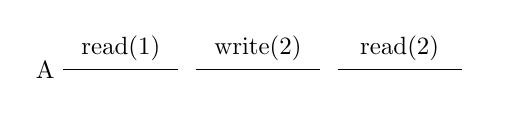
\begin{tikzpicture}[scale=0.9, transform shape] 
		\node (x1)  {A};
		\node (x2) [right of=x1,xshift=1cm]{};
		\draw (x1) -- node[above]{read(1)} (x2);
		\node(x3)[right of=x2,xshift=-1cm]{};
		\node(x4) [right of=x3,xshift=1cm]{};
		\draw (x3) -- node[above]{write(2)} (x4);
		
		\node(x5)[right of=x4,xshift=-1cm]{};
		\node(x6) [right of=x5,xshift=1cm]{};
		\draw (x5) -- node[above]{read(2)} (x6);
		\end{tikzpicture}
		\caption{A history of a sequential object}
\end{figure}
\end{frame}

\begin{frame}{Linearizability - Examples}
\begin{figure}[htp]
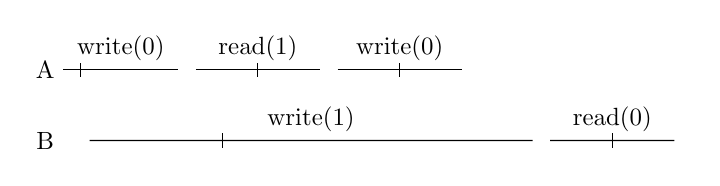
\begin{tikzpicture}[scale=0.9, transform shape] 
		\node (x1) {A};
		\node (x2) [right of=x1,xshift=1cm]{};
		\draw (x1) -- node[above]{write(0)} (x2);
		\draw (0.5,-0.1) -- (0.5,+0.1);
		
		\node(x3)[right of=x2,xshift=-1cm]{};
		\node(x4) [right of=x3,xshift=1cm]{};
		\draw (x3) -- node[above]{read(1)} (x4);
		\draw (3,-0.1) -- (3,+0.1);
		
		\node(x5)[right of=x4,xshift=-1cm]{};
		\node(x6) [right of=x5,xshift=1cm]{};
		\draw (x5) -- node[above]{write(0)} (x6);
		\draw (5,-0.1) -- (5,+0.1);
		
		\node(B)[below of=x1]{B};
		\node(x7)[below of=x1,xshift=0.5cm]{};
		\node(x8) [right of=x7,xshift=5.5cm]{};
		\draw (x7) -- node[above]{write(1)} (x8);
		\draw (2.5,-1.1) -- (2.5,-0.9);
		
		\node(x9)[right of=x8,xshift=-1cm]{};
		\node(x10) [right of=x9,xshift=1cm]{};
		\draw (x9) -- node[above]{read(0)} (x10);
		\draw (8,-1.1) -- (8,-0.9);
		
		\end{tikzpicture}
		\caption{A history of a concurrent object - linearizable}
\end{figure}
\end{frame}

\begin{frame}{Linearizability - Examples}
\begin{figure}[htp]
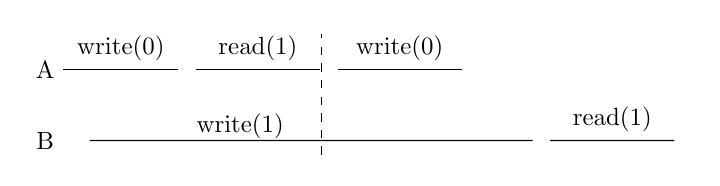
\begin{tikzpicture}[scale=0.9, transform shape] 
		\node (x1) {A};
		\node (x2) [right of=x1,xshift=1cm]{};
		\draw (x1) -- node[above]{write(0)} (x2);
		
		\node(x3)[right of=x2,xshift=-1cm]{};
		\node(x4) [right of=x3,xshift=1cm]{};
		\draw (x3) -- node[above]{read(1)} (x4);
		\draw[dashed] (3.9,-1.2) -- (3.9,+0.5);
		
		\node(x5)[right of=x4,xshift=-1cm]{};
		\node(x6) [right of=x5,xshift=1cm]{};
		\draw (x5) -- node[above]{write(0)} (x6);
		
		\node(B)[below of=x1]{B};
		\node(x7)[below of=x1,xshift=0.5cm]{};
		\node(x8) [right of=x7,xshift=5.5cm]{};
		\draw (x7) -- node [above, xshift=-1cm,yshift=-0.1cm] {write(1)} (x8);
		
		\node(x9)[right of=x8,xshift=-1cm]{};
		\node(x10) [right of=x9,xshift=1cm]{};
		\draw (x9) -- node[above]{read(1)} (x10);
		
		\end{tikzpicture}
		\caption{A history of a concurrent object - not linearizable}
\end{figure}
\end{frame}

\section{Binary Search Tree}
\begin{frame}{Binary Search Tree - Defintion}
A \textit{binary search tree} (BST) is a data structure which meets the following requirements:
\begin{itemize}
\item it  is a binary tree (a node can contain atmost two children)
\item each node contains a key $k$
\item left subtree of a node contains keys lesser than $k$
\item right subtree of a node contains keys greater than $k$
\end{itemize}
\pause
Operations on a BST
\begin{itemize}
\item \textbf{search($k$)} - returns \textit{true} only if key $k$ is present in the tree
\item \textbf{insert($k$)} - inserts $k$ into the tree if it does not already exist
\item \textbf{delete($k$)} - deletes $k$ from the tree if it already exist
\end{itemize}
\end{frame}

\begin{frame}{BST - Search}
\textbf{search($70$)}\\
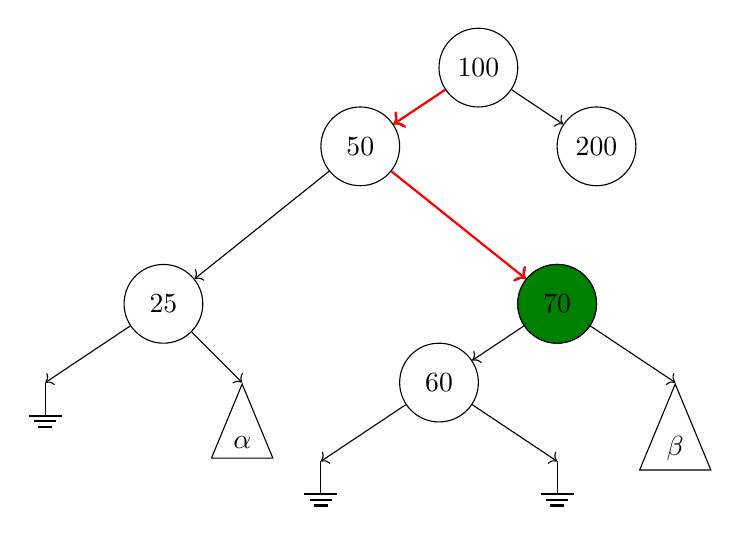
\begin{tikzpicture}
\newcommand\xShift{1.5}
\newcommand\yShift{1}
\node(x) [treenode] at (0, 0) {100};
\node(xl) [treenode] at ([shift=({-\xShift,-\yShift})]x) {50};
\node(xr) [treenode] at ([shift=({\xShift,-\yShift})]x) {200};
\node(xll) [treenode] at ([shift=({-\xShift-1,-\yShift-1})]xl) {25};
\node(xlr) [treenode] at ([shift=({\xShift+1,-\yShift-1})]xl) {70};
\node(xlll) [ground] at ([shift=({-\xShift,-\yShift})]xll) {};
\node(xllr) [subtree] at ([shift=({\xShift-0.5,-\yShift})]xll) {$\alpha$};
\node(xlrl) [treenode] at ([shift=({-\xShift,-\yShift})]xlr) {60};
\node(xlrr) [subtree] at ([shift=({\xShift,-\yShift})]xlr) {$\beta$};
\node(xlrll) [ground] at ([shift=({-\xShift,-\yShift})]xlrl) {};
\node(xlrlr) [ground] at ([shift=({\xShift,-\yShift})]xlrl) {};
\draw[->] (x) -- (xl);
\draw[->] (x) -- (xr);
\draw[->] (xl) -- (xll);
\draw[->] (xl) -- (xlr);
\draw[->] (xll) -- (xlll);
\draw[->] (xll) -- (xllr.north);
\draw[->] (xlr) -- (xlrl);
\draw[->] (xlr) -- (xlrr.north);
\draw[->] (xlrl) -- (xlrll);
\draw[->] (xlrl) -- (xlrlr);
\draw<2->[->,thick,color=red] (x) -- (xl);
\draw<3->[->,thick,color=red] (xl) -- (xlr);
\node<4->(xlr) [treenode,fill=black!50!green] at ([shift=({\xShift+1,-\yShift-1})]xl) {70};
\end{tikzpicture}
\end{frame}

\begin{frame}{BST - Search}
\textbf{search($55$)}\\
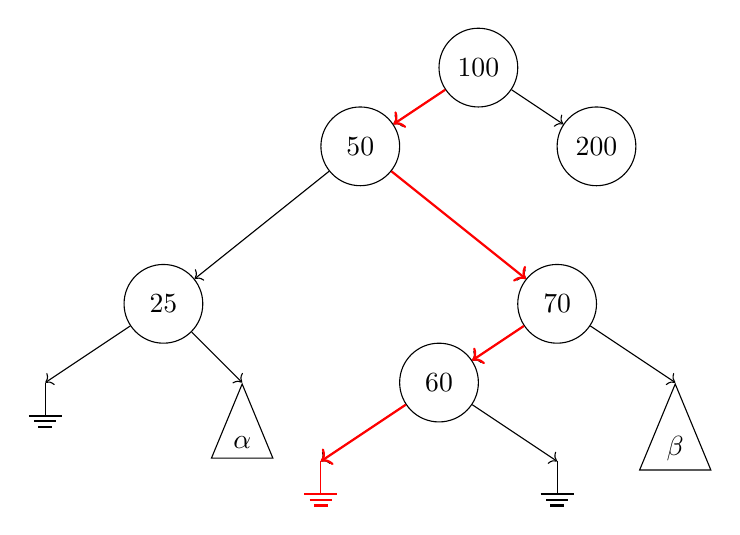
\begin{tikzpicture}
\newcommand\xShift{1.5}
\newcommand\yShift{1}
\node(x) [treenode] at (0, 0) {100};
\node(xl) [treenode] at ([shift=({-\xShift,-\yShift})]x) {50};
\node(xr) [treenode] at ([shift=({\xShift,-\yShift})]x) {200};
\node(xll) [treenode] at ([shift=({-\xShift-1,-\yShift-1})]xl) {25};
\node(xlr) [treenode] at ([shift=({\xShift+1,-\yShift-1})]xl) {70};
\node(xlll) [ground] at ([shift=({-\xShift,-\yShift})]xll) {};
\node(xllr) [subtree] at ([shift=({\xShift-0.5,-\yShift})]xll) {$\alpha$};
\node(xlrl) [treenode] at ([shift=({-\xShift,-\yShift})]xlr) {60};
\node(xlrr) [subtree] at ([shift=({\xShift,-\yShift})]xlr) {$\beta$};
\node(xlrll) [ground] at ([shift=({-\xShift,-\yShift})]xlrl) {};
\node(xlrlr) [ground] at ([shift=({\xShift,-\yShift})]xlrl) {};
\draw[->] (x) -- (xl);
\draw[->] (x) -- (xr);
\draw[->] (xl) -- (xll);
\draw[->] (xl) -- (xlr);
\draw[->] (xll) -- (xlll);
\draw[->] (xll) -- (xllr.north);
\draw[->] (xlr) -- (xlrl);
\draw[->] (xlr) -- (xlrr.north);
\draw[->] (xlrl) -- (xlrll);
\draw[->] (xlrl) -- (xlrlr);
\draw<2->[->,thick,color=red] (x) -- (xl);
\draw<3->[->,thick,color=red] (xl) -- (xlr);
\draw<4->[->,thick,color=red] (xlr) -- (xlrl);
\draw<5->[->,thick,color=red] (xlrl) -- (xlrll);
\node<6->(xlrll) [ground,color=red] at ([shift=({-\xShift,-\yShift})]xlrl) {};
\end{tikzpicture}
\end{frame}

\begin{frame}{BST - Insert}
\textbf{insert($55$)}\\
\begin{columns}
\begin{column}[t]{0.48\textwidth}
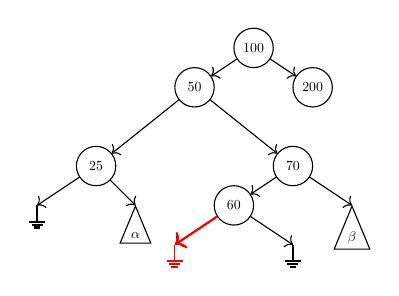
\begin{tikzpicture}[scale=0.5, transform shape]
\newcommand\xShift{1.5}
\newcommand\yShift{1}
\node(x) [treenode] at (0, 0) {100};
\node(xl) [treenode] at ([shift=({-\xShift,-\yShift})]x) {50};
\node(xr) [treenode] at ([shift=({\xShift,-\yShift})]x) {200};
\node(xll) [treenode] at ([shift=({-\xShift-1,-\yShift-1})]xl) {25};
\node(xlr) [treenode] at ([shift=({\xShift+1,-\yShift-1})]xl) {70};
\node(xlll) [ground] at ([shift=({-\xShift,-\yShift})]xll) {};
\node(xllr) [subtree] at ([shift=({\xShift-0.5,-\yShift})]xll) {$\alpha$};
\node(xlrl) [treenode] at ([shift=({-\xShift,-\yShift})]xlr) {60};
\node(xlrr) [subtree] at ([shift=({\xShift,-\yShift})]xlr) {$\beta$};
\node(xlrll) [ground] at ([shift=({-\xShift,-\yShift})]xlrl) {};
\node(xlrlr) [ground] at ([shift=({\xShift,-\yShift})]xlrl) {};
\draw[->] (x) -- (xl);
\draw[->] (x) -- (xr);
\draw[->] (xl) -- (xll);
\draw[->] (xl) -- (xlr);
\draw[->] (xll) -- (xlll);
\draw[->] (xll) -- (xllr.north);
\draw[->] (xlr) -- (xlrl);
\draw[->] (xlr) -- (xlrr.north);
\draw[->] (xlrl) -- (xlrll);
\draw[->] (xlrl) -- (xlrlr);
\draw<2->[->,thick,color=red] (xlrl) -- (xlrll);
\node<2->(xlrll) [ground,color=red] at ([shift=({-\xShift,-\yShift})]xlrl) {};
\end{tikzpicture}
\end{column}
\pause
\pause
\begin{column}[t]{0.5\textwidth}
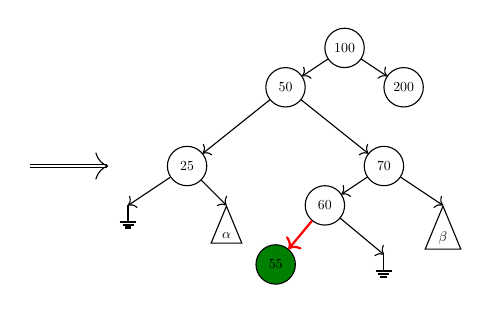
\begin{tikzpicture}[scale=0.5, transform shape]
\draw[->,style=double] (-8,-3) -- (-6,-3){};
\newcommand\xShift{1.5}
\newcommand\yShift{1}
\node(x) [treenode] at (0, 0) {100};
\node(xl) [treenode] at ([shift=({-\xShift,-\yShift})]x) {50};
\node(xr) [treenode] at ([shift=({\xShift,-\yShift})]x) {200};
\node(xll) [treenode] at ([shift=({-\xShift-1,-\yShift-1})]xl) {25};
\node(xlr) [treenode] at ([shift=({\xShift+1,-\yShift-1})]xl) {70};
\node(xlll) [ground] at ([shift=({-\xShift,-\yShift})]xll) {};
\node(xllr) [subtree] at ([shift=({\xShift-0.5,-\yShift})]xll) {$\alpha$};
\node(xlrl) [treenode] at ([shift=({-\xShift,-\yShift})]xlr) {60};
\node(xlrr) [subtree] at ([shift=({\xShift,-\yShift})]xlr) {$\beta$};
\node(xlrll) [treenode,fill=black!50!green] at ([shift=({-\xShift+0.25,-\yShift-0.5})]xlrl) {55};
\node(xlrlr) [ground] at ([shift=({\xShift,-\yShift-0.25})]xlrl) {};
\draw[->] (x) -- (xl);
\draw[->] (x) -- (xr);
\draw[->] (xl) -- (xll);
\draw[->] (xl) -- (xlr);
\draw[->] (xll) -- (xlll);
\draw[->] (xll) -- (xllr.north);
\draw[->] (xlr) -- (xlrl);
\draw[->] (xlr) -- (xlrr.north);
\draw[->,thick,color=red] (xlrl) -- (xlrll);
\draw[->] (xlrl) -- (xlrlr);
\end{tikzpicture}
\end{column}
\end{columns}
\end{frame}

\begin{frame}{Types of delete}
\begin{itemize}
\item simple - removing a node which has atmost one child
\item complex - removing a node which has exactly two children
\end{itemize}
\end{frame}

\begin{frame}{BST - Simple Delete}
\textbf{delete($25$)}
\begin{figure}[b]
\begin{columns}
\begin{column}[t]{0.48\textwidth}
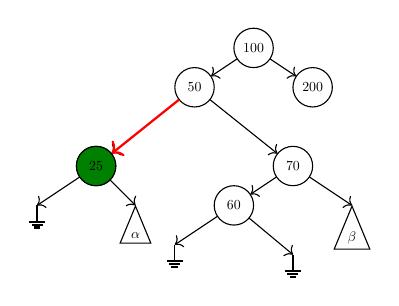
\begin{tikzpicture}[scale=0.5, transform shape]
\newcommand\xShift{1.5}
\newcommand\yShift{1}
\node(x) [treenode] at (0, 0) {100};
\node(xl) [treenode] at ([shift=({-\xShift,-\yShift})]x) {50};
\node(xr) [treenode] at ([shift=({\xShift,-\yShift})]x) {200};
\node(xll) [treenode] at ([shift=({-\xShift-1,-\yShift-1})]xl) {25};
\node(xlr) [treenode] at ([shift=({\xShift+1,-\yShift-1})]xl) {70};
\node(xlll) [ground] at ([shift=({-\xShift,-\yShift})]xll) {};
\node(xllr) [subtree] at ([shift=({\xShift-0.5,-\yShift})]xll) {$\alpha$};
\node(xlrl) [treenode] at ([shift=({-\xShift,-\yShift})]xlr) {60};
\node(xlrr) [subtree] at ([shift=({\xShift,-\yShift})]xlr) {$\beta$};
\node(xlrll) [ground] at ([shift=({-\xShift,-\yShift})]xlrl) {};
\node(xlrlr) [ground] at ([shift=({\xShift,-\yShift-0.25})]xlrl) {};
\draw[->] (x) -- (xl);
\draw[->] (x) -- (xr);
\draw[->] (xl) -- (xll);
\draw[->] (xl) -- (xlr);
\draw[->] (xll) -- (xlll);
\draw[->] (xll) -- (xllr.north);
\draw[->] (xlr) -- (xlrl);
\draw[->] (xlr) -- (xlrr.north);
\draw[->] (xlrl) -- (xlrll);
\draw[->] (xlrl) -- (xlrlr);
\draw<2->[->,thick,color=red] (xl) -- (xll);
\node<2->(xll) [treenode,fill=black!50!green] at ([shift=({-\xShift-1,-\yShift-1})]xl) {25};
\end{tikzpicture}
\end{column}
\pause
\pause
\begin{column}[t]{0.5\textwidth}
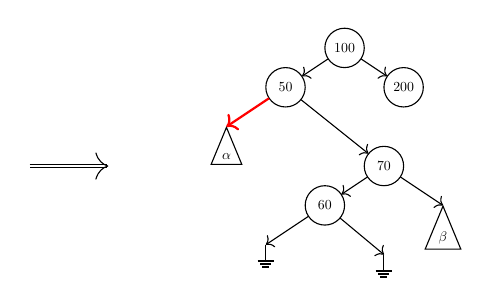
\begin{tikzpicture}[scale=0.5, transform shape]
\draw[->,style=double] (-8,-3) -- (-6,-3){};
\newcommand\xShift{1.5}
\newcommand\yShift{1}
\node(x) [treenode] at (0, 0) {100};
\node(xl) [treenode] at ([shift=({-\xShift,-\yShift})]x) {50};
\node(xr) [treenode] at ([shift=({\xShift,-\yShift})]x) {200};
\node(xll) [subtree] at ([shift=({-\xShift,-\yShift})]xl) {$\alpha$};
\node(xlr) [treenode] at ([shift=({\xShift+1,-\yShift-1})]xl) {70};
\node(xlrl) [treenode] at ([shift=({-\xShift,-\yShift})]xlr) {60};
\node(xlrr) [subtree] at ([shift=({\xShift,-\yShift})]xlr) {$\beta$};
\node(xlrll) [ground] at ([shift=({-\xShift,-\yShift})]xlrl) {};
\node(xlrlr) [ground] at ([shift=({\xShift,-\yShift-0.25})]xlrl) {};
\draw[->] (x) -- (xl);
\draw[->] (x) -- (xr);
\draw[->,thick,color=red] (xl) -- (xll.north);
\draw[->] (xl) -- (xlr);
\draw[->] (xlr) -- (xlrl);
\draw[->] (xlr) -- (xlrr.north);
\draw[->] (xlrl) -- (xlrll);
\draw[->] (xlrl) -- (xlrlr);
\end{tikzpicture}
\end{column}
\end{columns}
\end{figure}
\end{frame}

\begin{frame}{BST - Complex Delete}
\textbf{delete($50$)}
\begin{figure}[b]
\begin{columns}
\begin{column}[t]{0.33\textwidth}
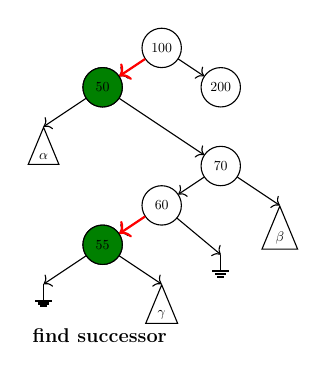
\begin{tikzpicture}[scale=0.5, transform shape]
\newcommand\xShift{1.5}
\newcommand\yShift{1}
\node(x) [treenode] at (0, 0) {100};
\node(xl) [treenode] at ([shift=({-\xShift,-\yShift})]x) {50};
\node(xr) [treenode] at ([shift=({\xShift,-\yShift})]x) {200};
\node(xll) [subtree] at ([shift=({-\xShift,-\yShift})]xl) {$\alpha$};
\node(xlr) [treenode] at ([shift=({\xShift+1.5,-\yShift-1})]xl) {70};
\node(xlrl) [treenode] at ([shift=({-\xShift,-\yShift})]xlr) {60};
\node(xlrr) [subtree] at ([shift=({\xShift,-\yShift})]xlr) {$\beta$};
\node(xlrll) [treenode] at ([shift=({-\xShift,-\yShift})]xlrl) {55};
\node(xlrlr) [ground] at ([shift=({\xShift,-\yShift-0.25})]xlrl) {};
\node(xlrlll) [ground] at ([shift=({-\xShift,-\yShift})]xlrll) {};
\node(xlrllr) [subtree] at ([shift=({\xShift,-\yShift})]xlrll) {$\gamma$};
\draw[->] (x) -- (xl);
\draw[->] (x) -- (xr);
\draw[->] (xl) -- (xll.north);
\draw[->] (xl) -- (xlr);
\draw[->] (xlr) -- (xlrl);
\draw[->] (xlr) -- (xlrr.north);
\draw[->] (xlrl) -- (xlrll);
\draw[->] (xlrl) -- (xlrlr);
\draw[->] (xlrll) -- (xlrlll);
\draw[->] (xlrll) -- (xlrllr.north);
\draw<2->[->,thick,color=red] (x) -- (xl);
\node<2->(xl) [treenode,fill=black!50!green] at ([shift=({-\xShift,-\yShift})]x) {50};
\draw<3->[->,thick,color=red] (xlrl) -- (xlrll);
\node<3->(xlrll) [treenode,fill=black!50!green] at ([shift=({-\xShift,-\yShift})]xlrl) {55};
\node<3->[below right] at (current bounding box.south west) {\Large \textbf{find successor}};
\end{tikzpicture}
\end{column}
\pause
\pause
\pause
\begin{column}[t]{0.33\textwidth}
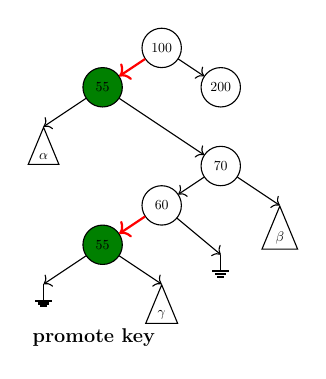
\begin{tikzpicture}[scale=0.5, transform shape]
%\draw[->,style=double] (-8,-3) -- (-7,-3){};
\newcommand\xShift{1.5}
\newcommand\yShift{1}
\node(x) [treenode] at (0, 0) {100};
\node(xl) [treenode,fill=black!50!green] at ([shift=({-\xShift,-\yShift})]x) {55};
\node(xr) [treenode] at ([shift=({\xShift,-\yShift})]x) {200};
\node(xll) [subtree] at ([shift=({-\xShift,-\yShift})]xl) {$\alpha$};
\node(xlr) [treenode] at ([shift=({\xShift+1.5,-\yShift-1})]xl) {70};
\node(xlrl) [treenode] at ([shift=({-\xShift,-\yShift})]xlr) {60};
\node(xlrr) [subtree] at ([shift=({\xShift,-\yShift})]xlr) {$\beta$};
\node(xlrll) [treenode,fill=black!50!green] at ([shift=({-\xShift,-\yShift})]xlrl) {55};
\node(xlrlr) [ground] at ([shift=({\xShift,-\yShift-0.25})]xlrl) {};
\node(xlrlll) [ground] at ([shift=({-\xShift,-\yShift})]xlrll) {};
\node(xlrllr) [subtree] at ([shift=({\xShift,-\yShift})]xlrll) {$\gamma$};
\draw[->,thick,color=red] (x) -- (xl);
\draw[->] (x) -- (xr);
\draw[->] (xl) -- (xll.north);
\draw[->] (xl) -- (xlr);
\draw[->] (xlr) -- (xlrl);
\draw[->] (xlr) -- (xlrr.north);
\draw[->,thick,color=red] (xlrl) -- (xlrll);
\draw[->] (xlrl) -- (xlrlr);
\draw[->] (xlrll) -- (xlrlll);
\draw[->] (xlrll) -- (xlrllr.north);
\node[below right] at (current bounding box.south west) {\Large \textbf{promote key}};
\end{tikzpicture}
\end{column}
\pause
\begin{column}[t]{0.33\textwidth}
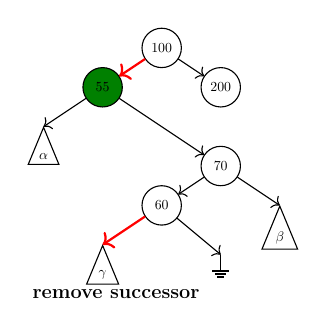
\begin{tikzpicture}[scale=0.5, transform shape]
%\draw[->,style=double] (-8,-3) -- (-7,-3){};
\newcommand\xShift{1.5}
\newcommand\yShift{1}
\node(x) [treenode] at (0, 0) {100};
\node(xl) [treenode,fill=black!50!green] at ([shift=({-\xShift,-\yShift})]x) {55};
\node(xr) [treenode] at ([shift=({\xShift,-\yShift})]x) {200};
\node(xll) [subtree] at ([shift=({-\xShift,-\yShift})]xl) {$\alpha$};
\node(xlr) [treenode] at ([shift=({\xShift+1.5,-\yShift-1})]xl) {70};
\node(xlrl) [treenode] at ([shift=({-\xShift,-\yShift})]xlr) {60};
\node(xlrr) [subtree] at ([shift=({\xShift,-\yShift})]xlr) {$\beta$};
\node(xlrll) [subtree] at ([shift=({-\xShift,-\yShift})]xlrl) {$\gamma$};
\node(xlrlr) [ground] at ([shift=({\xShift,-\yShift-0.25})]xlrl) {};
\draw[->,thick,color=red] (x) -- (xl);
\draw[->] (x) -- (xr);
\draw[->] (xl) -- (xll.north);
\draw[->] (xl) -- (xlr);
\draw[->] (xlr) -- (xlrl);
\draw[->] (xlr) -- (xlrr.north);
\draw[->,thick,color=red] (xlrl) -- (xlrll.north);
\draw[->] (xlrl) -- (xlrlr);
\node<3->[below right] at (current bounding box.south west) {\Large \textbf{remove successor}};
\end{tikzpicture}
\end{column}
\end{columns}
\end{figure}
\end{frame}

\section{Related Works}
\begin{comment}
\begin{frame}{Related Works}
\begin{itemize}
\item lock-free(node-based) external BST by Ellen et.al[PODC'10]
\item lock-free(node-based) internal BST by Howley and Jones[SPAA'12]
\item lock-free(edge-based) external BST by Natarajan and Mittal[PPoPP'14]
\item RCU-based(node-based) internal BST by Arbel and Attiya[PODC'14]
\item lock-based(node-based) internal BST by Drachsler et.al[PPoPP'14]
\end{itemize}
\end{frame}
\end{comment}
\begin{frame}{Related Works}
\begin{table}[h]
\small{
\begin{tabular}{|l|l|c|c|l|}
\hline
\textbf{\#} & \multicolumn{1}{c|}{\textbf{\begin{tabular}[c]{@{}c@{}}Algorithm\\ Type\end{tabular}}} & \textbf{\begin{tabular}[c]{@{}c@{}}Works\\ At\end{tabular}} & \textbf{\begin{tabular}[c]{@{}c@{}}BST\\ Type\end{tabular}} & \multicolumn{1}{c|}{\textbf{Authors}} \\ \hline
1           & lock free                                                                              & node level                                                  & external                                                    & Ellen et.al{[}PODC'10{]}              \\ \hline
2           & lock free                                                                              & node level                                                  & internal                                                    & Howley \& Jones{[}SPAA'12{]}          \\ \hline
3           & lock free                                                                              & edge level                                                  & external                                                    & Natarajan \&Mittal{[}PPoPP'14{]}      \\ \hline
4           & lock based                                                                             & node level                                                  & internal                                                    & Arbel \& Attiya{[}PODC'14{]}          \\ \hline
5           & lock based                                                                             & node level                                                  & internal                                                    & Drachsler et.al{[}PPoPP'14{]}         \\ \hline
\end{tabular}
}
\end{table}
\end{frame}

\section{Lock Based Binary Search Tree}
\begin{frame}[c]{Lock Based BST[PPoPP'15 Poster]}
Contributions
\begin{itemize}
\item combine edge-based locking with internal representation of BST
\item optimistic tree traversal 
\end{itemize}
\end{frame}

\begin{frame}[c]{Lock Based BST[PPoPP'15 Poster]}
\begin{itemize}
\item common workloads have more searches than updates
\begin{itemize}
\item design is optimized for searches
\item search operations are oblivious to locks
\end{itemize}
\pause
\item Any real life workload will have more inserts than deletes
\begin{itemize}
\item insert operations do not obtain any locks
\item performs only one atomic operation
\end{itemize}
\pause
\item removal of a node in a concurrent BST is challenging
\begin{itemize}
\item delete operations uses locks
\item locks can be obtained on nodes or edges
\item locking edges instead of nodes increases concurrency
\end{itemize}
\end{itemize}
\end{frame}

\begin{frame}{Lock Based BST - Challenges in search}
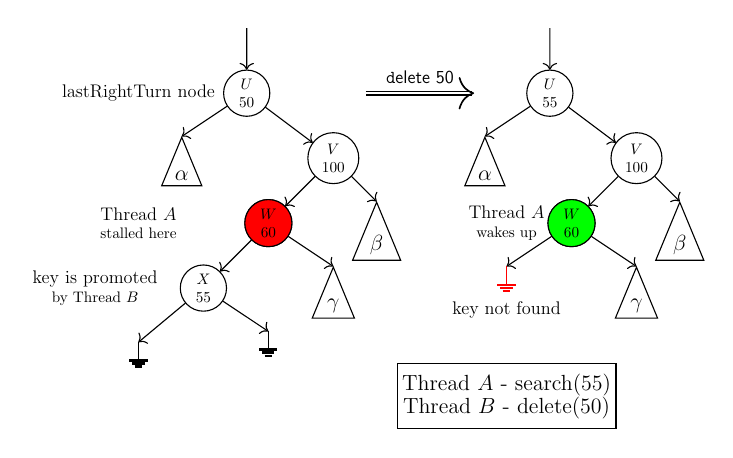
\begin{tikzpicture}[scale=0.55, transform shape,mylabel/.style={thin, draw=black, align=center, minimum width=0.3cm, minimum height=0.3cm,fill=white}]
		\newcommand\XA{0}
		\newcommand\YA{0}
		\node (x)		[treenode] 									at (-6,0)       							{$U$ \\ 50};
		\node (a)		[subtree] 									at (-7.5,-1)  								{\Large $\alpha$};
		\node (y0)	[treenode] 									at (-4,-1.5) 									{$V$ \\ 100};
		\node (y1)	[treenode]									at (-5.5,-3)									{$W$ \\ 60}; 
		\node (b)		[subtree] 									at (-3,-2.5)    							{\Large $\beta$};
		\node (y2)	[treenode]									at (-7,-4.5)									{$X$ \\ 55}; 
		\node (g)		[subtree] 									at (-4,-4)   									{\Large $\gamma$};
		\node (gnd)	[ground] 										at (-8.5,-5.75)								{}; 
		\node (o)		[ground] 										at (-5.5,-5.5)  							{};
		\node (x1) 	[] 													at (-8.5,0) 									{\large lastRightTurn node};
		\draw[->] (-6, 1.5) --  (x);
		\draw[->] (x) -- (y0);
		\draw[->] (x) -- (a.north);
		\draw[->] (y0) -- (y1);
		\draw[->] (y0) -- (b.north);
		\draw[->] (y1) -- (y2);
		\draw[->] (y1) -- (g.north);
		\draw[->] (y2) -- (gnd);
		\draw[->] (y2) -- (o);
		%% legend
		\node [thin, draw=black, align=center, minimum width=5cm, minimum height=1.5cm] at (0,-7) {\Large Thread $A$ - search(55) \\ \Large Thread $B$ - delete(50)};	
		\pause
		\node (y1)	[treenode, fill=red]		at (-5.5,-3)											{$W$ \\ 60}; 
		\node (y1l) [rectangle,align=center,minimum size=1cm] at (-8.5,-3) 		{\large Thread $A$ \\stalled here};
		\pause
		\node (y2l) [rectangle,align=center,minimum size=1cm] at(-9.5,-4.5) 	{\large key is promoted \\by Thread $B$};
		\pause
		\path[every node/.style={font=\sffamily\small}]
		(-3.25, 0) edge[->,semithick, double] node [above, outer sep=3pt] 		{\large \texttt delete 50} (-0.75, 0);

		\node (ix)	[treenode] 									at (1,0)       								{$U$ \\ 55};
		\node (ia)	[subtree] 									at (-0.5,-1)  								{\Large $\alpha$};
		\node (iy0)	[treenode] 									at (3,-1.5) 									{$V$ \\ 100};
		\node (iy1)	[treenode, fill=red]									at (1.5,-3)					{$W$ \\ 60}; 
		\node (ib)	[subtree] 									at (4,-2.5)    								{\Large $\beta$};
		\node (io)	[ground]										at (0,-4)											{}; 
		\node (ignd)[subtree] 									at (3,-4)   									{\Large $\gamma$};
    
    \draw[->] (1, 1.5) --  (ix);
    \draw[->] (ix) --  (iy0);
    \draw[->] (ix) --  (ia.north);
    \draw[->] (iy0) --  (iy1);
    \draw[->] (iy0) --  (ib.north);
    \draw[->] (iy1) --  (io);
    \draw[->] (iy1) --  (ignd.north);
		\pause
		\node (iy1)	[treenode, fill=green]									at (1.5,-3)					{$W$ \\ 60};
		\node (y12) [rectangle,align=center,minimum size=1cm] at (0,-3) 		{\large Thread $A$ \\wakes up};
		\pause
		\node (io)	[ground,color=red]										at (0,-4)											{}; 
		\node (y13) [rectangle,align=center,minimum size=1cm] at (0,-5) 		{\large key not found};
	\end{tikzpicture}
\visible<6>
{
\\Keep track of last right turn node and its key. If search terminates at a NULL node, check if the current key in the last right turn node has changed. If yes restart the operation from root.
}
\end{frame}

\ifdefined\LONG
\begin{frame}[c]{Lock Based BST - Delete}
pseudocode for delete
\begin{algorithm}[H]
locate the node to delete\;
\uIf{simple delete}
{
lock the edge $\langle$parent,node$\rangle$\;
lock the children edges\;
make the parent point to the non-null child using a simple write instruction\;
release all locks\;
}
\Else(// complex delete)
{
lock the edge $\langle$node,rightChild$\rangle$\;
find the successor\;
lock the edge $\langle$successorParent,successor$\rangle$\;
lock the children edges of successor\;
promote key\;
remove successor by a making successorParent point to non-null child of successor\;
release all locks\;
}
\end{algorithm}
\end{frame}
\fi

\begin{frame}[c]{Lock Based BST - Simple Delete}
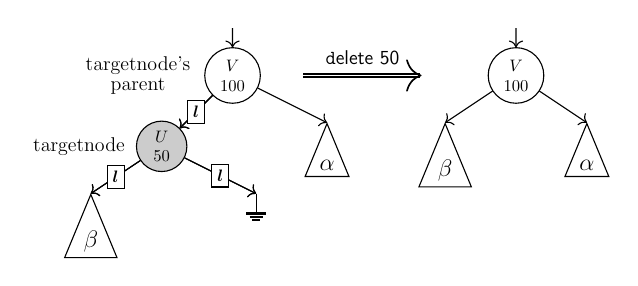
\begin{tikzpicture}[scale=0.6, transform shape,mylabel/.style={thin, draw=black, align=center, minimum width=0.3cm, minimum height=0.3cm,fill=white}]
		\newcommand\XA{-3}
		\newcommand\YA{0}
		\node (x)		[treenode] 																at (\XA,\YA)       					{$V$ \\ 100};
		\node (y)		[treenode, fill=black!20] 								at (\XA-1.5,\YA-1.5) 				{$U$ \\ 50};
		\node (a)		[subtree] 																at (\XA+2,\YA-1)      			{\Large $\alpha$};
		\node (b)		[subtree] 																at (\XA-3,\YA-2.5)    			{\Large $\beta$};
		\node (gnd)	[ground] 																	at (\XA+0.5,\YA-2.5)				{}; 
		\node (xl) 	[rectangle,align=center,minimum size=1cm] at (\XA-2,\YA) 							{\large targetnode's \\ \large parent};
		\node (yl) 	[] 																				at (\XA-3.25,\YA-1.5) 			{\large targetnode};
		
 		\draw[->] (x) -- (y);
 		\draw[->] (y) -- (b.north);
 		\draw[->] (y) -- (gnd);
		\draw[->] (\XA,\YA+1) -- (x);
		\draw[->] (x) -- (a.north);
		\pause
		\draw[->] (x) -- node[mylabel] {$\boldsymbol{l}$} (y);
		\pause
		\draw[->] (y) -- node[mylabel] {$\boldsymbol{l}$} (b.north);
		\pause
		\draw[->] (y) -- node[mylabel] {$\boldsymbol{l}$} (gnd);
    \pause
		\path[every node/.style={font=\sffamily\small}]
		(\XA+1.5,\YA) edge[->,semithick, double] 							node [above, outer sep=3pt] {\large \texttt delete 50} (\XA+4,\YA);
		
		\node (ix)	[treenode] 																at (\XA+6,\YA) 							{$V$ \\ 100};
		\node (ib)	[subtree] 																at (\XA+4.5,\YA-1)					{\Large $\beta$};
		\node (ia)	[subtree] 																at (\XA+7.5,\YA-1) 					{\Large $\alpha$};

		\draw[->] (\XA+6,\YA+1) -- (ix);
		\draw[->] (ix) -- (ib.north);
		\draw[->] (ix) -- (ia.north);
	\end{tikzpicture}
\end{frame}

\begin{frame}[c]{Lock Based BST - Complex Delete}
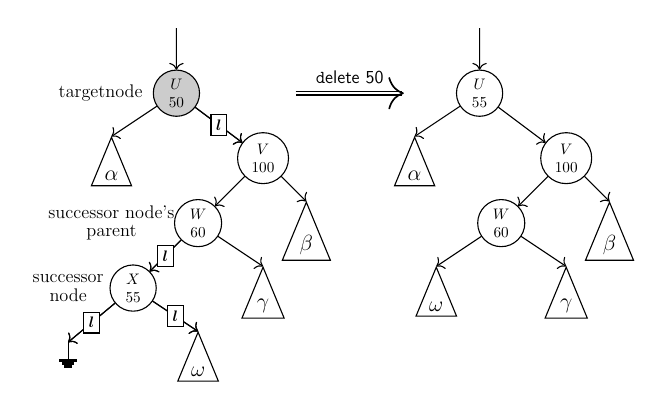
\begin{tikzpicture}[scale=0.55, transform shape,mylabel/.style={thin, draw=black, align=center, minimum width=0.3cm, minimum height=0.3cm,fill=white}]
		\newcommand\XA{0}
		\newcommand\YA{0}
		\node (x)		[treenode, fill=black!20] 	at (-6,0)       							{$U$ \\ 50};
		\node (a)		[subtree] 									at (-7.5,-1)  								{\Large $\alpha$};
		\node (y0)	[treenode] 									at (-4,-1.5) 									{$V$ \\ 100};
		\node (y1)	[treenode]									at (-5.5,-3)									{$W$ \\ 60}; 
		\node (b)		[subtree] 									at (-3,-2.5)    							{\Large $\beta$};
		\node (y2)	[treenode]									at (-7,-4.5)									{$X$ \\ 55}; 
		\node (g)		[subtree] 									at (-4,-4)   									{\Large $\gamma$};
		\node (gnd)	[ground] 										at (-8.5,-5.75)									{}; 
		\node (o)		[subtree] 									at (-5.5,-5.5)  							{\Large $\omega$};
		\node (x1) 	[] 													at (-7.75,0) 									{\large targetnode};
		\node (y1l) [rectangle,align=center,minimum size=1cm] at (-7.5,-3) 		{\large successor node's \\ \large parent};
		\node (y2l) [rectangle,align=center,minimum size=1cm] at(-8.5,-4.5) 	{\large successor \\ \large node};
		
		\draw[->] (-6, 1.5) --  (x);
		\draw[->] (x) -- (y0);
		\draw[->] (x) -- (a.north);
		\draw[->] (y0) -- (y1);
		\draw[->] (y0) -- (b.north);
		\draw[->] (y1) -- (y2);
		\draw[->] (y1) -- (g.north);
		\draw[->] (y2) -- (gnd);
		\draw[->] (y2) -- (o.north);
    \pause
    \draw[->] (x) -- node[mylabel] {$\boldsymbol{l}$} (y0);
    \pause
    \draw[->] (y1) -- node[mylabel] {$\boldsymbol{l}$} (y2);
    \pause
    \draw[->] (y2) -- node[mylabel] {$\boldsymbol{l}$} (gnd);
    \pause
  	\draw[->] (y2) -- node[mylabel] {$\boldsymbol{l}$} (o.north);
    \pause
		\path[every node/.style={font=\sffamily\small}]
		(-3.25, 0) edge[->,semithick, double] node [above, outer sep=3pt] 		{\large \texttt delete 50} (-0.75, 0);

		\node (ix)	[treenode] 									at (1,0)       								{$U$ \\ 55};
		\node (ia)	[subtree] 									at (-0.5,-1)  								{\Large $\alpha$};
		\node (iy0)	[treenode] 									at (3,-1.5) 									{$V$ \\ 100};
		\node (iy1)	[treenode]									at (1.5,-3)										{$W$ \\ 60}; 
		\node (ib)	[subtree] 									at (4,-2.5)    								{\Large $\beta$};
		\node (io)	[subtree]										at (0,-4)											{\Large $\omega$}; 
		\node (ignd)[subtree] 									at (3,-4)   									{\Large $\gamma$};
    
    \draw[->] (1, 1.5) --  (ix);
    \draw[->] (ix) --  (iy0);
    \draw[->] (ix) --  (ia.north);
    \draw[->] (iy0) --  (iy1);
    \draw[->] (iy0) --  (ib.north);
    \draw[->] (iy1) --  (io.north);
    \draw[->] (iy1) --  (ignd.north);
	\end{tikzpicture}
\end{frame}

\begin{frame}{Lock Based BST - More challenges in search}
A scenario in which the last right turn node is removed
\begin{figure}
\centering
{
	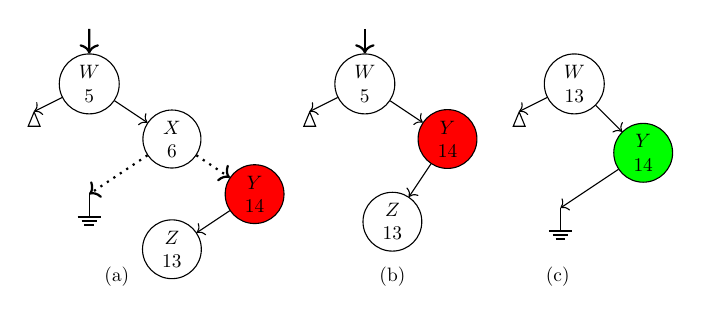
\begin{tikzpicture}[scale=0.7, transform shape]
		\newcommand\XA{-5}
		\newcommand\YA{0}
		\node[] at (-4.5,-3.5) {(a)};
		\node (x)		[treenode] 									at (\XA,\YA)       						{$W$ \\ 5};
		\node (S1)	[subtree,scale=0.5] 				at ([shift=({-1,-0.5})]x)  		{};
		\node (y0)	[treenode] 									at ([shift=({1.5,-1})]x) 			{$X$ \\ 6};
		\node (gnd)	[ground]										at ([shift=({-1.5,-1})]y0)		{}; 
		\node (y1)	[treenode,fill=red] 				at ([shift=({1.5,-1})]y0)   	{$Y$ \\ 14};
		\node (y2)	[treenode] 									at ([shift=({-1.5,-1})]y1)  	{$Z$ \\ 13};
		%\node (S2)	[subtree,scale=0.5]					at ([shift=({0.5,-1})]y1)			{}; 

		\path[every node/.style={font=\sffamily\large}]
		(\XA,\YA+1) 	edge[->,thick] 		node 					{} (x)
		(x) 		edge[->]								node 					{} (S1.north)
		(x) 		edge[->]								node 					{} (y0)
		(y0) 		edge[->,dotted,thick]		node 					{} (gnd)
		(y0) 		edge[->,dotted,thick]		node 					{} (y1)
		(y1) 		edge[->]								node 					{} (y2);
		%(y1) 		edge[->]							node 					{} (S2.north);
		\pause
		\renewcommand\XA{0}
		\node[] at (0.5,-3.5) {(b)};
		\node (ix)	[treenode] 										at (\XA,\YA)       						{$W$ \\ 5};
		\node (iS1)	[subtree,scale=0.5] 					at ([shift=({-1,-0.5})]ix)  	{};
		\node (iy1)	[treenode,fill=red] 					at ([shift=({1.5,-1})]ix)   	{$Y$ \\ 14};
		\node (iy2)	[treenode] 										at ([shift=({-1,-1.5})]iy1)  	{$Z$ \\ 13};
		%\node (iS2)	[subtree,scale=0.5]					at ([shift=({0.5,-1.0})]iy1)	{}; 

		\path[every node/.style={font=\sffamily\large}]
		(\XA,\YA+1) 	edge[->,thick] 		node 					{} (ix)
		(ix) 		edge[->]								node 					{} (iS1.north)
		(ix) 		edge[->]								node 					{} (iy1)
		(iy1) 	edge[->]								node 					{} (iy2);
		%(iy1) 	edge[->]								node 					{} (iS2.north);
		\pause
		\renewcommand\XA{3.8}
		\node[] at (3.5,-3.5) {(c)};
		\node (iix)		[treenode] 									at (\XA,\YA)       							{$W$ \\ 13};
		\node (iiS1)	[subtree,scale=0.5] 				at ([shift=({-1,-0.5})]iix)  		{};
		\node (iiy1)	[treenode,fill=green] 			at ([shift=({1.25,-1.25})]iix)  {$Y$ \\ 14};
		\node (iignd)	[ground]										at ([shift=({-1.5,-1})]iiy1)		{}; 
		
		\path[every node/.style={font=\sffamily\large}]
		(iix) 		edge[->]								node 					{} (iiS1.north)
		(iix) 		edge[->]								node 					{} (iiy1)
		(iiy1) 		edge[->]								node 					{} (iignd);	
	\end{tikzpicture}
}
\end{figure}

\begin{itemize}
\item<1> \footnotesize Search(13) gets stalled at $Y$ in (a). Its last right turn node is $X$
\item<2> \footnotesize Delete(6) removes $X$ from the tree in (b). The key stored in $X$ is still 6
\item<3> \footnotesize Delete(5) results in 13 moving up the tree from $Z$ to $W$ in (c). When search(13) wakes up, it will miss 13 as the key in the last right turn node has not changed
\end{itemize}


\begin{itemize}
\item<4> \footnotesize In the first traversal search(13) saw the node $X$
\item<4> \footnotesize In the second traversal there are two cases
\begin{itemize}
\item<4> \tiny case1, search(13) did not find $X$ - save the traversal and restart
\item<4> \tiny case2, search(13) did find $X$ - use the results of previous traversal
\end{itemize}
\end{itemize}

\end{frame}

\section{Lock Free Binary Search Tree}
\begin{frame}[c]{Lock Free BST[ICDCN'15]}
Contributions
\begin{itemize}
\item combine edge-based locking with internal representation of BST 
\item optimistic tree traversal 
\pause
\item lock-free algorithm
\end{itemize}
\end{frame}

\begin{frame}{Lock Free BST[ICDCN'15]}
\begin{itemize}
\item search and inserts are same as in lock Based BST
\item to maintain lock-free property, if an insert or delete operation fails, it helps a pending delete operation(if needed)
\end{itemize} 
pseudocode for delete
\begin{algorithm}[H]
locate the node to delete\;
flag the children edges for deletion\;
\uIf{simple delete}
{
make the parent point to the non-null child atomically\;
}
\Else(// complex delete)
{
find the successor\;
flag the children edges of successor for promotion\;
promote key\;
remove successor by a simple delete\;
replace node with a fresh copy\;
}
\end{algorithm}
\end{frame}

\begin{frame}[c]{Lock Free BST - Simple Delete}
\begin{itemize}
\item flag is owned by an operation
\item if a thread which installed the flag is stalled, other threads can help complete the operation
\end{itemize}
\pause
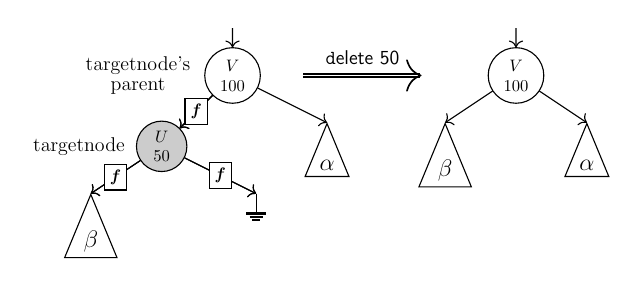
\begin{tikzpicture}[scale=0.6, transform shape,mylabel/.style={thin, draw=black, align=center, minimum width=0.3cm, minimum height=0.3cm,fill=white}]
		\newcommand\XA{-3}
		\newcommand\YA{0}
		\node (x)		[treenode] 																at (\XA,\YA)       					{$V$ \\ 100};
		\node (y)		[treenode, fill=black!20] 								at (\XA-1.5,\YA-1.5) 				{$U$ \\ 50};
		\node (a)		[subtree] 																at (\XA+2,\YA-1)      			{\Large $\alpha$};
		\node (b)		[subtree] 																at (\XA-3,\YA-2.5)    			{\Large $\beta$};
		\node (gnd)	[ground] 																	at (\XA+0.5,\YA-2.5)				{}; 
		\node (xl) 	[rectangle,align=center,minimum size=1cm] at (\XA-2,\YA) 							{\large targetnode's \\ \large parent};
		\node (yl) 	[] 																				at (\XA-3.25,\YA-1.5) 			{\large targetnode};
		
 		\draw[->] (x) -- (y);
 		\draw[->] (y) -- (b.north);
 		\draw[->] (y) -- (gnd);
		\draw[->] (\XA,\YA+1) -- (x);
		\draw[->] (x) -- (a.north);
		\pause
		%% legend
		%\node (l1) 																						at (\XA+4.5,\YA-3){\Large $\boldsymbol{i}$  - \Large intent flag set};
		%\node (l2) 																						at (\XA+4.5,\YA-3.5){\Large $\boldsymbol{d}$  - \Large delete flag set};
		%\node [thin, draw=black, align=center, minimum width=5cm, minimum height=1.25cm] at (\XA+5,\YA-3.15) {};	
		%\draw[->] (x) -- node[mylabel] {$\boldsymbol{i}$} (y);
		\draw[->] (x) -- node[mylabel] {$\boldsymbol{f}$} (y);
		\pause
		%\draw[->] (y) -- node[mylabel] {$\boldsymbol{d}$} (b.north);
		\draw[->] (y) -- node[mylabel] {$\boldsymbol{f}$} (b.north);
		\pause
		%\draw[->] (y) -- node[mylabel] {$\boldsymbol{d}$} (gnd);
		\draw[->] (y) -- node[mylabel] {$\boldsymbol{f}$} (gnd);
    \pause
		\path[every node/.style={font=\sffamily\small}]
		(\XA+1.5,\YA) edge[->,semithick, double] 							node [above, outer sep=3pt] {\large \texttt delete 50} (\XA+4,\YA);
		
		\node (ix)	[treenode] 																at (\XA+6,\YA) 							{$V$ \\ 100};
		\node (ib)	[subtree] 																at (\XA+4.5,\YA-1)					{\Large $\beta$};
		\node (ia)	[subtree] 																at (\XA+7.5,\YA-1) 					{\Large $\alpha$};

		\draw[->] (\XA+6,\YA+1) -- (ix);
		\draw[->] (ix) -- (ib.north);
		\draw[->] (ix) -- (ia.north);
	\end{tikzpicture}
\end{frame}

\begin{frame}[c]{Lock Free BST - Complex Delete}
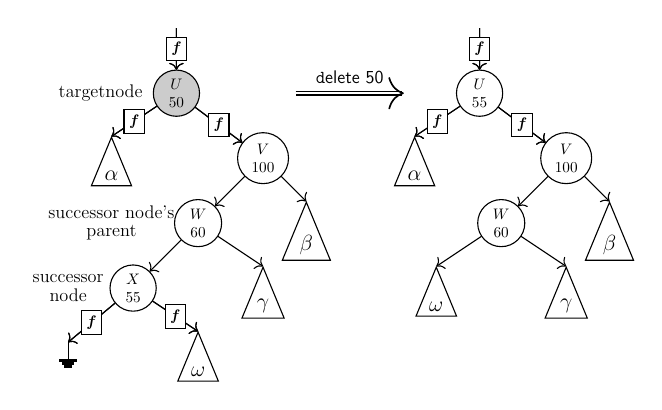
\begin{tikzpicture}[scale=0.55, transform shape,mylabel/.style={thin, draw=black, align=center, minimum width=0.3cm, minimum height=0.3cm,fill=white}]
		\newcommand\XA{0}
		\newcommand\YA{0}
		\node (x)		[treenode, fill=black!20] 	at (-6,0)       							{$U$ \\ 50};
		\node (a)		[subtree] 									at (-7.5,-1)  								{\Large $\alpha$};
		\node (y0)	[treenode] 									at (-4,-1.5) 									{$V$ \\ 100};
		\node (y1)	[treenode]									at (-5.5,-3)									{$W$ \\ 60}; 
		\node (b)		[subtree] 									at (-3,-2.5)    							{\Large $\beta$};
		\node (y2)	[treenode]									at (-7,-4.5)									{$X$ \\ 55}; 
		\node (g)		[subtree] 									at (-4,-4)   									{\Large $\gamma$};
		\node (gnd)	[ground] 										at (-8.5,-5.75)									{}; 
		\node (o)		[subtree] 									at (-5.5,-5.5)  							{\Large $\omega$};
		\node (x1) 	[] 													at (-7.75,0) 									{\large targetnode};
		\node (y1l) [rectangle,align=center,minimum size=1cm] at (-7.5,-3) 		{\large successor node's \\ \large parent};
		\node (y2l) [rectangle,align=center,minimum size=1cm] at(-8.5,-4.5) 	{\large successor \\ \large node};
		\draw[->] (-6, 1.5) --  (x);
		\draw[->] (x) -- (y0);
		\draw[->] (x) -- (a.north);
		\draw[->] (y0) -- (y1);
		\draw[->] (y0) -- (b.north);
		\draw[->] (y1) -- (y2);
		\draw[->] (y1) -- (g.north);
		\draw[->] (y2) -- (gnd);
		\draw[->] (y2) -- (o.north);
    \pause
		\draw[->] (-6, 1.5) -- node[mylabel] {$\boldsymbol{f}$} (x);
    \pause
		\draw[->] (x) -- node[mylabel] {$\boldsymbol{f}$} (a.north);
    \pause
		\draw[->] (x) -- node[mylabel] {$\boldsymbol{f}$} (y0);
    \pause
		\draw[->] (y2) -- node[mylabel] {$\boldsymbol{f}$} (gnd);
    \pause
		\draw[->] (y2) -- node[mylabel] {$\boldsymbol{f}$} (o.north);
    \pause
		\path[every node/.style={font=\sffamily\small}]
		(-3.25, 0) edge[->,semithick, double] node [above, outer sep=3pt] 		{\large \texttt delete 50} (-0.75, 0);
		\node (ix)	[treenode] 									at (1,0)       								{$U$ \\ 55};
		\node (ia)	[subtree] 									at (-0.5,-1)  								{\Large $\alpha$};
		\node (iy0)	[treenode] 									at (3,-1.5) 									{$V$ \\ 100};
		\node (iy1)	[treenode]									at (1.5,-3)										{$W$ \\ 60}; 
		\node (ib)	[subtree] 									at (4,-2.5)    								{\Large $\beta$};
		\node (io)	[subtree]										at (0,-4)											{\Large $\omega$}; 
		\node (ignd)[subtree] 									at (3,-4)   									{\Large $\gamma$};
    
    \draw[->] (1, 1.5) --  (ix);
    \draw[->] (ix) --  (iy0);
    \draw[->] (ix) --  (ia.north);
    \draw[->] (iy0) --  (iy1);
    \draw[->] (iy0) --  (ib.north);
    \draw[->] (iy1) --  (io.north);
    \draw[->] (iy1) --  (ignd.north);
		\draw[->] (1, 1.5) -- node[mylabel] {$\boldsymbol{f}$} (ix);
		\draw[->] (ix) -- node[mylabel] {$\boldsymbol{f}$} (ia.north);
		\draw[->] (ix) -- node[mylabel] {$\boldsymbol{f}$} (iy0);
	\end{tikzpicture}
\end{frame}
\begin{frame}[c]{Lock Free BST - Complex Delete}
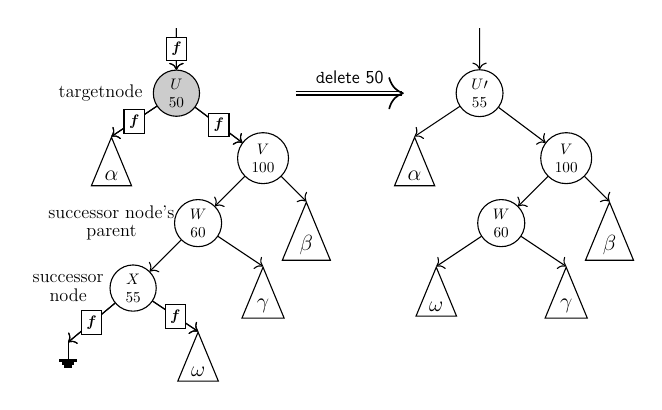
\begin{tikzpicture}[scale=0.55, transform shape,mylabel/.style={thin, draw=black, align=center, minimum width=0.3cm, minimum height=0.3cm,fill=white}]
		\newcommand\XA{0}
		\newcommand\YA{0}
		\node (x)		[treenode, fill=black!20] 	at (-6,0)       							{$U$ \\ 50};
		\node (a)		[subtree] 									at (-7.5,-1)  								{\Large $\alpha$};
		\node (y0)	[treenode] 									at (-4,-1.5) 									{$V$ \\ 100};
		\node (y1)	[treenode]									at (-5.5,-3)									{$W$ \\ 60}; 
		\node (b)		[subtree] 									at (-3,-2.5)    							{\Large $\beta$};
		\node (y2)	[treenode]									at (-7,-4.5)									{$X$ \\ 55}; 
		\node (g)		[subtree] 									at (-4,-4)   									{\Large $\gamma$};
		\node (gnd)	[ground] 										at (-8.5,-5.75)									{}; 
		\node (o)		[subtree] 									at (-5.5,-5.5)  							{\Large $\omega$};
		\node (x1) 	[] 													at (-7.75,0) 									{\large targetnode};
		\node (y1l) [rectangle,align=center,minimum size=1cm] at (-7.5,-3) 		{\large successor node's \\ \large parent};
		\node (y2l) [rectangle,align=center,minimum size=1cm] at(-8.5,-4.5) 	{\large successor \\ \large node};
		\draw[->] (-6, 1.5) --  (x);
		\draw[->] (x) -- (y0);
		\draw[->] (x) -- (a.north);
		\draw[->] (y0) -- (y1);
		\draw[->] (y0) -- (b.north);
		\draw[->] (y1) -- (y2);
		\draw[->] (y1) -- (g.north);
		\draw[->] (y2) -- (gnd);
		\draw[->] (y2) -- (o.north);
		\draw[->] (-6, 1.5) -- node[mylabel] {$\boldsymbol{f}$} (x);
		\draw[->] (x) -- node[mylabel] {$\boldsymbol{f}$} (a.north);
		\draw[->] (x) -- node[mylabel] {$\boldsymbol{f}$} (y0);
		\draw[->] (y2) -- node[mylabel] {$\boldsymbol{f}$} (gnd);
		\draw[->] (y2) -- node[mylabel] {$\boldsymbol{f}$} (o.north);
		\path[every node/.style={font=\sffamily\small}]
		(-3.25, 0) edge[->,semithick, double] node [above, outer sep=3pt] 		{\large \texttt delete 50} (-0.75, 0);
		\node (ix)	[treenode] 									at (1,0)       								{$U\prime$ \\ 55};
		\node (ia)	[subtree] 									at (-0.5,-1)  								{\Large $\alpha$};
		\node (iy0)	[treenode] 									at (3,-1.5) 									{$V$ \\ 100};
		\node (iy1)	[treenode]									at (1.5,-3)										{$W$ \\ 60}; 
		\node (ib)	[subtree] 									at (4,-2.5)    								{\Large $\beta$};
		\node (io)	[subtree]										at (0,-4)											{\Large $\omega$}; 
		\node (ignd)[subtree] 									at (3,-4)   									{\Large $\gamma$};
    
    \draw[->] (1, 1.5) --  (ix);
    \draw[->] (ix) --  (iy0);
    \draw[->] (ix) --  (ia.north);
    \draw[->] (iy0) --  (iy1);
    \draw[->] (iy0) --  (ib.north);
    \draw[->] (iy1) --  (io.north);
    \draw[->] (iy1) --  (ignd.north);
	\end{tikzpicture}
\end{frame}

\section{Local recovery}
\begin{frame}[c]{Local recovery[PPoPP'16 Poster]}
Overview
\begin{itemize}
\item a general technique for local recovery for concurrent BSTs
\item reduces tree traversal cost during failures by restarting closer to an operation�s window
\end{itemize}
Motivation
\begin{itemize}
\item in most concurrent BSTs, execution phase of an operation have constant time complexity
\item seek phase is where an operation may end up spending most of its time (esp for large trees)
\item this technique reduces the seek time
\end{itemize}
\end{frame}

\begin{frame}[c]{Example}
\begin{figure}[htp]
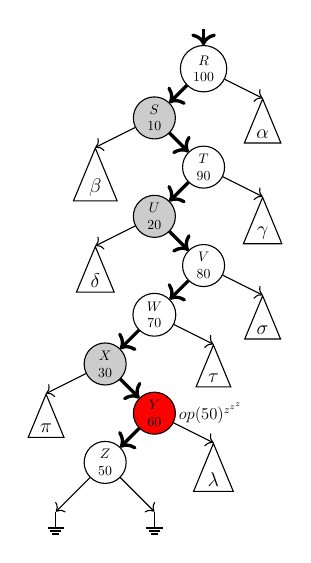
\begin{tikzpicture}[scale=0.5, transform shape] 
	 \newcommand\NODEDX{1.25}
	 \newcommand\NODEDY{1.25}
	 \newcommand\SUBTREEDX{1.5}
	 \newcommand\SUBTREEDY{0.75}
	
   \node (r)	[treenode] 		                at (0, 0)       		                      	{$R$ \\ 100};
   \node (s)	[treenode, fill=black!20] 		at ([shift=({ -\NODEDX, -\NODEDY})]r)     	{$S$ \\ 10};
	 \node (t)	[treenode] 		                at ([shift=({  \NODEDX, -\NODEDY})]s)    		{$T$ \\ 90};
	 \node (u)	[treenode, fill=black!20] 	  at ([shift=({ -\NODEDX, -\NODEDY})]t)     	{$U$ \\ 20};
	 \node (v)	[treenode] 										at ([shift=({  \NODEDX, -\NODEDY})]u)     	{$V$ \\ 80};
	 \node (w)	[treenode] 										at ([shift=({ -\NODEDX, -\NODEDY})]v)     	{$W$ \\ 70};
	 \node (x)	[treenode, fill=black!20] 		at ([shift=({ -\NODEDX, -\NODEDY})]w)     	{$X$ \\ 30};
	 \node (y)	[treenode,fill=red]						at ([shift=({  \NODEDX, -\NODEDY})]x)     	{$Y$ \\ 60};
	 \node (z)	[treenode] 										at ([shift=({ -\NODEDX, -\NODEDY})]y)     	{$Z$ \\ 50};
	 \node (gl) [ground]                      at ([shift=({ -\NODEDX, -\NODEDY})]z)     	{ };
	 \node (gr) [ground]                      at ([shift=({  \NODEDX, -\NODEDY})]z)     	{ };
		
	 \node (sa) [subtree]                     at ([shift=({  \SUBTREEDX, -\SUBTREEDY})]r) {\Large $\alpha$};
	 \node (sb) [subtree]                     at ([shift=({ -\SUBTREEDX, -\SUBTREEDY})]s) {\Large $\beta$};
	 \node (sg) [subtree]                     at ([shift=({  \SUBTREEDX, -\SUBTREEDY})]t) {\Large $\gamma$};
	 \node (sd) [subtree]                     at ([shift=({ -\SUBTREEDX, -\SUBTREEDY})]u) {\Large $\delta$};
	 \node (ss) [subtree]                     at ([shift=({  \SUBTREEDX, -\SUBTREEDY})]v) {\Large $\sigma$};
	 \node (st) [subtree]                     at ([shift=({  \SUBTREEDX, -\SUBTREEDY})]w) {\Large $\tau$};
	 \node (sp) [subtree]                     at ([shift=({ -\SUBTREEDX, -\SUBTREEDY})]x) {\Large $\pi$};
	 \node (sl) [subtree]                     at ([shift=({  \SUBTREEDX, -\SUBTREEDY})]y) {\Large $\lambda$};	
	
	 \node (op) [label={right:{\large $op(50)^{z^{z^z}}$}}] at ([shift=({0.375, 0})]y) {};
	
	 \path[every node/.style={font=\sffamily\small}]
	    (0, 1)  edge[->,very thick]  node {} (r)
		  (r)     edge[->,very thick]  node {} (s)
			(s)     edge[->,very thick]  node {} (t)
			(t)     edge[->,very thick]  node {} (u)
			(u)     edge[->,very thick]  node {} (v)
			(v)     edge[->,very thick]  node {} (w)
			(w)     edge[->,very thick]  node {} (x)
			(x)     edge[->,very thick]  node {} (y)
			(y)     edge[->,very thick]  node {} (z)
			(z)     edge[->]  node {} (gl)
			(z)     edge[->]  node {} (gr)
			(r)     edge[->]  node {} (sa.north)
			(s)     edge[->]  node {} (sb.north)
			(t)     edge[->]  node {} (sg.north)
			(u)     edge[->]  node {} (sd.north)
			(v)     edge[->]  node {} (ss.north)
			(w)     edge[->]  node {} (st.north)
			(x)     edge[->]  node {} (sp.north)
			(y)     edge[->]  node {} (sl.north);		
\end{tikzpicture}
\caption{Operation $op(50)$ is suspended at node $Y$ during its traversal}
\end{figure}
\end{frame}

\begin{frame}[c]{Example}
\begin{figure}[htp]
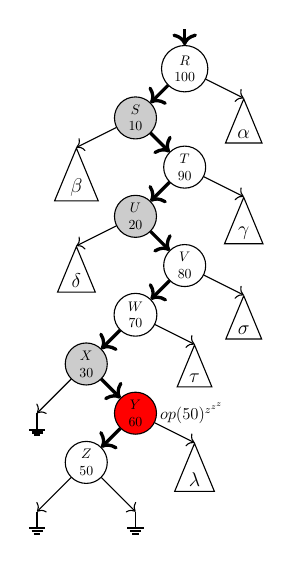
\begin{tikzpicture}[scale=0.5, transform shape]   
	 \newcommand\NODEDX{1.25}
	 \newcommand\NODEDY{1.25}
	 \newcommand\SUBTREEDX{1.5}
	 \newcommand\SUBTREEDY{0.75}
	
   \node (r)	[treenode] 		                at (0, 0)       		                      	{$R$ \\ 100};
   \node (s)	[treenode, fill=black!20] 		at ([shift=({ -\NODEDX, -\NODEDY})]r)     	{$S$ \\ 10};
	 \node (t)	[treenode] 		                at ([shift=({  \NODEDX, -\NODEDY})]s)    		{$T$ \\ 90};
	 \node (u)	[treenode, fill=black!20] 	  at ([shift=({ -\NODEDX, -\NODEDY})]t)     	{$U$ \\ 20};
	 \node (v)	[treenode] 										at ([shift=({  \NODEDX, -\NODEDY})]u)     	{$V$ \\ 80};
	 \node (w)	[treenode] 										at ([shift=({ -\NODEDX, -\NODEDY})]v)     	{$W$ \\ 70};
	 \node (x)	[treenode, fill=black!20] 		at ([shift=({ -\NODEDX, -\NODEDY})]w)     	{$X$ \\ 30};
	 \node (y)	[treenode, fill=red]					at ([shift=({  \NODEDX, -\NODEDY})]x)     	{$Y$ \\ 60};
	 \node (z)	[treenode] 										at ([shift=({ -\NODEDX, -\NODEDY})]y)     	{$Z$ \\ 50};
	 \node (gl) [ground]                      at ([shift=({ -\NODEDX, -\NODEDY})]z)     	{ };
	 \node (gr) [ground]                      at ([shift=({  \NODEDX, -\NODEDY})]z)     	{ };

	 \node (sa) [subtree]                     at ([shift=({  \SUBTREEDX, -\SUBTREEDY})]r) {\Large $\alpha$};
	 \node (sb) [subtree]                     at ([shift=({ -\SUBTREEDX, -\SUBTREEDY})]s) {\Large $\beta$};
	 \node (sg) [subtree]                     at ([shift=({  \SUBTREEDX, -\SUBTREEDY})]t) {\Large $\gamma$};
	 \node (sd) [subtree]                     at ([shift=({ -\SUBTREEDX, -\SUBTREEDY})]u) {\Large $\delta$};
	 \node (ss) [subtree]                     at ([shift=({  \SUBTREEDX, -\SUBTREEDY})]v) {\Large $\sigma$};
	 \node (st) [subtree]                     at ([shift=({  \SUBTREEDX, -\SUBTREEDY})]w) {\Large $\tau$};
	 %% \node (sp) [subtree]                     at ([shift=({ -\SUBTREEDX, -\SUBTREEDY})]x) {\Large $\pi$};
	 \node (sp) [ground]                    	at ([shift=({ -\NODEDX, -\NODEDY})]x) { };
	 \node (sl) [subtree]                     at ([shift=({  \SUBTREEDX, -\SUBTREEDY})]y) {\Large $\lambda$};	

   \node (op) [label={right:{\large $op(50)^{z^{z^z}}$}}] at ([shift=({0.375, 0})]y) {};
	
	 \path[every node/.style={font=\sffamily\small}]
	    (0, 1)  edge[->,very thick]  node {} (r)
		  (r)     edge[->,very thick]  node {} (s)
			(s)     edge[->,very thick]  node {} (t)
			(t)     edge[->,very thick]  node {} (u)
			(u)     edge[->,very thick]  node {} (v)
			(v)     edge[->,very thick]  node {} (w)
			(w)     edge[->,very thick]  node {} (x)
			(x)     edge[->,very thick]  node {} (y)
			(y)     edge[->,very thick]  node {} (z)
			(z)     edge[->]  node {} (gl)
			(z)     edge[->]  node {} (gr)
			(r)     edge[->]  node {} (sa.north)
			(s)     edge[->]  node {} (sb.north)
			(t)     edge[->]  node {} (sg.north)
			(u)     edge[->]  node {} (sd.north)
			(v)     edge[->]  node {} (ss.north)
			(w)     edge[->]  node {} (st.north)
			(x)     edge[->]  node {} (sp)
			(y)     edge[->]  node {} (sl.north);	
\end{tikzpicture}
\caption{All keys in subtree $\pi$ are deleted one-by-one}
\end{figure}
\end{frame}

\begin{frame}[c]{Example}
\begin{figure}[htp]
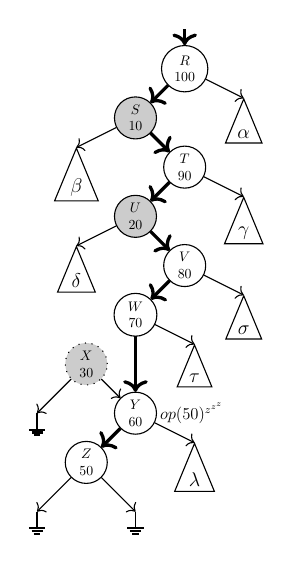
\begin{tikzpicture}[scale=0.5, transform shape]
   
	 \newcommand\NODEDX{1.25}
	 \newcommand\NODEDY{1.25}
	 \newcommand\SUBTREEDX{1.5}
	 \newcommand\SUBTREEDY{0.75}
	
   \node (r)	[treenode] 		                at (0, 0)       		                      	{$R$ \\ 100};
   \node (s)	[treenode, fill=black!20] 		at ([shift=({ -\NODEDX, -\NODEDY})]r)     	{$S$ \\ 10};
	 \node (t)	[treenode] 		                at ([shift=({  \NODEDX, -\NODEDY})]s)    		{$T$ \\ 90};
	 \node (u)	[treenode, fill=black!20] 	  at ([shift=({ -\NODEDX, -\NODEDY})]t)     	{$U$ \\ 20};
	 \node (v)	[treenode] 										at ([shift=({  \NODEDX, -\NODEDY})]u)     	{$V$ \\ 80};
	 \node (w)	[treenode] 										at ([shift=({ -\NODEDX, -\NODEDY})]v)     	{$W$ \\ 70};
	 \node (x)	[treenode, fill=black!20, dotted] 		at ([shift=({ -\NODEDX, -\NODEDY})]w)     	{$X$ \\ 30};
	 \node (y)	[treenode] 										at ([shift=({  \NODEDX, -\NODEDY})]x)     	{$Y$ \\ 60};
	 \node (z)	[treenode] 										at ([shift=({ -\NODEDX, -\NODEDY})]y)     	{$Z$ \\ 50};
	 \node (gl) [ground]                      at ([shift=({ -\NODEDX, -\NODEDY})]z)     	{ };
	 \node (gr) [ground]                      at ([shift=({  \NODEDX, -\NODEDY})]z)     	{ };
		
	 \node (sa) [subtree]                     at ([shift=({  \SUBTREEDX, -\SUBTREEDY})]r) {\Large $\alpha$};
	 \node (sb) [subtree]                     at ([shift=({ -\SUBTREEDX, -\SUBTREEDY})]s) {\Large $\beta$};
	 \node (sg) [subtree]                     at ([shift=({  \SUBTREEDX, -\SUBTREEDY})]t) {\Large $\gamma$};
	 \node (sd) [subtree]                     at ([shift=({ -\SUBTREEDX, -\SUBTREEDY})]u) {\Large $\delta$};
	 \node (ss) [subtree]                     at ([shift=({  \SUBTREEDX, -\SUBTREEDY})]v) {\Large $\sigma$};
	 \node (st) [subtree]                     at ([shift=({  \SUBTREEDX, -\SUBTREEDY})]w) {\Large $\tau$};
	 %% \node (sp) [subtree]                     at ([shift=({ -\SUBTREEDX, -\SUBTREEDY})]x) {\Large $\pi$};
	 \node (sp) [ground]                    	at ([shift=({ -\NODEDX, -\NODEDY})]x) { };
	 \node (sl) [subtree]                     at ([shift=({  \SUBTREEDX, -\SUBTREEDY})]y) {\Large $\lambda$};	
	
	 \node (op) [label={right:{\large $op(50)^{z^{z^z}}$}}] at ([shift=({0.375, 0})]y) {};
	
	 \path[every node/.style={font=\sffamily\small}]
	    (0, 1)  edge[->,very thick]  node {} (r)
		  (r)     edge[->,very thick]  node {} (s)
			(s)     edge[->,very thick]  node {} (t)
			(t)     edge[->,very thick]  node {} (u)
			(u)     edge[->,very thick]  node {} (v)
			(v)     edge[->,very thick]  node {} (w)
			%% (w)     edge[->]  node {} (x)
			(w)     edge[->,very thick]  node {} (y)
			(x)     edge[->]  node {} (y)
			(y)     edge[->,very thick]  node {} (z)
			(z)     edge[->]  node {} (gl)
			(z)     edge[->]  node {} (gr)
			(r)     edge[->]  node {} (sa.north)
			(s)     edge[->]  node {} (sb.north)
			(t)     edge[->]  node {} (sg.north)
			(u)     edge[->]  node {} (sd.north)
			(v)     edge[->]  node {} (ss.north)
			(w)     edge[->]  node {} (st.north)
			(x)     edge[->]  node {} (sp)
			(y)     edge[->]  node {} (sl.north);	
\end{tikzpicture}
\caption{Key 30 is deleted (simple delete); node $X$ is removed}
\end{figure}
\end{frame}

\begin{frame}[c]{Example}
\begin{figure}[htp]
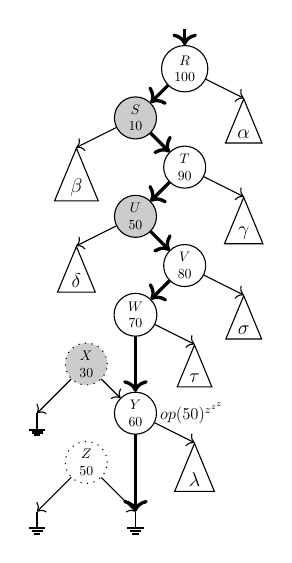
\begin{tikzpicture}[scale=0.5, transform shape]
   
	 \newcommand\NODEDX{1.25}
	 \newcommand\NODEDY{1.25}
	 \newcommand\SUBTREEDX{1.5}
	 \newcommand\SUBTREEDY{0.75}
	
   \node (r)	[treenode] 		                at (0, 0)       		                      	{$R$ \\ 100};
   \node (s)	[treenode, fill=black!20] 		at ([shift=({ -\NODEDX, -\NODEDY})]r)     	{$S$ \\ 10};
	 \node (t)	[treenode] 		                at ([shift=({  \NODEDX, -\NODEDY})]s)    		{$T$ \\ 90};
	 \node (u)	[treenode, fill=black!20] 	  at ([shift=({ -\NODEDX, -\NODEDY})]t)     	{$U$ \\ 50};
	 \node (v)	[treenode] 										at ([shift=({  \NODEDX, -\NODEDY})]u)     	{$V$ \\ 80};
	 \node (w)	[treenode] 										at ([shift=({ -\NODEDX, -\NODEDY})]v)     	{$W$ \\ 70};
	 \node (x)	[treenode, fill=black!20, dotted] 		at ([shift=({ -\NODEDX, -\NODEDY})]w)     	{$X$ \\ 30};
	 \node (y)	[treenode] 										at ([shift=({  \NODEDX, -\NODEDY})]x)     	{$Y$ \\ 60};
	 \node (z)	[treenode, dotted] 						at ([shift=({ -\NODEDX, -\NODEDY})]y)     	{$Z$ \\ 50};
	 \node (gl) [ground]                      at ([shift=({ -\NODEDX, -\NODEDY})]z)     	{ };
	 \node (gr) [ground]                      at ([shift=({  \NODEDX, -\NODEDY})]z)     	{ };
		
	 \node (sa) [subtree]                     at ([shift=({  \SUBTREEDX, -\SUBTREEDY})]r) {\Large $\alpha$};
	 \node (sb) [subtree]                     at ([shift=({ -\SUBTREEDX, -\SUBTREEDY})]s) {\Large $\beta$};
	 \node (sg) [subtree]                     at ([shift=({  \SUBTREEDX, -\SUBTREEDY})]t) {\Large $\gamma$};
	 \node (sd) [subtree]                     at ([shift=({ -\SUBTREEDX, -\SUBTREEDY})]u) {\Large $\delta$};
	 \node (ss) [subtree]                     at ([shift=({  \SUBTREEDX, -\SUBTREEDY})]v) {\Large $\sigma$};
	 \node (st) [subtree]                     at ([shift=({  \SUBTREEDX, -\SUBTREEDY})]w) {\Large $\tau$};
	 %% \node (sp) [subtree]                     at ([shift=({ -\SUBTREEDX, -\SUBTREEDY})]x) {\Large $\pi$};
	 \node (sp) [ground]                    	at ([shift=({ -\NODEDX, -\NODEDY})]x) { };
	 \node (sl) [subtree]                     at ([shift=({  \SUBTREEDX, -\SUBTREEDY})]y) {\Large $\lambda$};	
	
	 \node (op) [label={right:{\large $op(50)^{z^{z^z}}$}}] at ([shift=({0.375, 0})]y) {};
	
	 \path[every node/.style={font=\sffamily\small}]
	    (0, 1)  edge[->,very thick]  node {} (r)
		  (r)     edge[->,very thick]  node {} (s)
			(s)     edge[->,very thick]  node {} (t)
			(t)     edge[->,very thick]  node {} (u)
			(u)     edge[->,very thick]  node {} (v)
			(v)     edge[->,very thick]  node {} (w)
			%% (w)     edge[->]  node {} (x)
			(w)     edge[->,very thick]  node {} (y)
			(x)     edge[->]  node {} (y)
			%% (y)     edge[->]  node {} (z)
			(y)     edge[->, very thick]  node {} (gr)
			(z)     edge[->]  node {} (gl)
			(z)     edge[->]  node {} (gr)
			(r)     edge[->]  node {} (sa.north)
			(s)     edge[->]  node {} (sb.north)
			(t)     edge[->]  node {} (sg.north)
			(u)     edge[->]  node {} (sd.north)
			(v)     edge[->]  node {} (ss.north)
			(w)     edge[->]  node {} (st.north)
			(x)     edge[->]  node {} (sp)
			(y)     edge[->]  node {} (sl.north);		
\end{tikzpicture}
\caption{Key 20 is deleted (complex delete); key 20 is replaced with key 50 in node $U$ and node $Z$ is removed}
\end{figure}
\end{frame}

\begin{frame}[c]{Traversal Stack}
\begin{itemize}
\item a stack to keep track of anchor nodes of all nodes in the traversal path
\item reduces tree traversal cost during failures by restarting closer to an operation�s window
\end{itemize}
\end{frame}

\begin{frame}[c]{Traversal Stack}
\begin{figure}[htp]
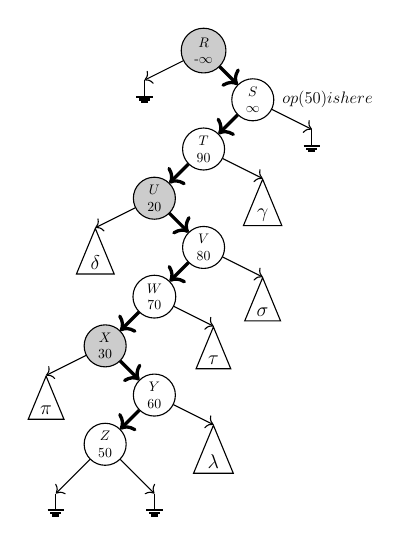
\begin{tikzpicture}[scale=0.5, transform shape] 
	 \newcommand\NODEDX{1.25}
	 \newcommand\NODEDY{1.25}
	 \newcommand\SUBTREEDX{1.5}
	 \newcommand\SUBTREEDY{0.75}
	
   \node (r)	[treenode, fill=black!20] 		at (0, 0)       		                      	{$R$ \\  -$\infty$};
   \node (s)	[treenode] 										at ([shift=({ \NODEDX, -\NODEDY})]r)     	  {$S$ \\  $\infty$};
	 \node (t)	[treenode] 		                at ([shift=({  -\NODEDX, -\NODEDY})]s)    	{$T$ \\ 90};
	 \node (u)	[treenode, fill=black!20] 	  at ([shift=({ -\NODEDX, -\NODEDY})]t)     	{$U$ \\ 20};
	 \node (v)	[treenode] 										at ([shift=({  \NODEDX, -\NODEDY})]u)     	{$V$ \\ 80};
	 \node (w)	[treenode] 										at ([shift=({ -\NODEDX, -\NODEDY})]v)     	{$W$ \\ 70};
	 \node (x)	[treenode, fill=black!20] 		at ([shift=({ -\NODEDX, -\NODEDY})]w)     	{$X$ \\ 30};
	 \node (y)	[treenode] 										at ([shift=({  \NODEDX, -\NODEDY})]x)     	{$Y$ \\ 60};
	 \node (z)	[treenode] 										at ([shift=({ -\NODEDX, -\NODEDY})]y)     	{$Z$ \\ 50};
	 \node (gl) [ground]                      at ([shift=({ -\NODEDX, -\NODEDY})]z)     	{ };
	 \node (gr) [ground]                      at ([shift=({  \NODEDX, -\NODEDY})]z)     	{ };
		
	 \node (sa) [ground]                      at ([shift=({ -\SUBTREEDX, -\SUBTREEDY})]r) { };
	 \node (sb) [ground]                      at ([shift=({ \SUBTREEDX, -\SUBTREEDY})]s) 	{ };
	 \node (sg) [subtree]                     at ([shift=({  \SUBTREEDX, -\SUBTREEDY})]t) {\Large $\gamma$};
	 \node (sd) [subtree]                     at ([shift=({ -\SUBTREEDX, -\SUBTREEDY})]u) {\Large $\delta$};
	 \node (ss) [subtree]                     at ([shift=({  \SUBTREEDX, -\SUBTREEDY})]v) {\Large $\sigma$};
	 \node (st) [subtree]                     at ([shift=({  \SUBTREEDX, -\SUBTREEDY})]w) {\Large $\tau$};
	 \node (sp) [subtree]                     at ([shift=({ -\SUBTREEDX, -\SUBTREEDY})]x) {\Large $\pi$};
	 \node (sl) [subtree]                     at ([shift=({  \SUBTREEDX, -\SUBTREEDY})]y) {\Large $\lambda$};	
	
	 \node (op) [label={right:{\large $op(50) is here$}}] at ([shift=({0.5, 0})]s) {};
	
	 \path[every node/.style={font=\sffamily\small}]
	    %(0, 1)  edge[->,very thick]  node {} (r)
		  (r)     edge[->,very thick]  node {} (s)
			(s)     edge[->,very thick]  node {} (t)
			(t)     edge[->,very thick]  node {} (u)
			(u)     edge[->,very thick]  node {} (v)
			(v)     edge[->,very thick]  node {} (w)
			(w)     edge[->,very thick]  node {} (x)
			(x)     edge[->,very thick]  node {} (y)
			(y)     edge[->,very thick]  node {} (z)
			(z)     edge[->]  node {} (gl)
			(z)     edge[->]  node {} (gr)
			(r)     edge[->]  node {} (sa)
			(s)     edge[->]  node {} (sb)
			(t)     edge[->]  node {} (sg.north)
			(u)     edge[->]  node {} (sd.north)
			(v)     edge[->]  node {} (ss.north)
			(w)     edge[->]  node {} (st.north)
			(x)     edge[->]  node {} (sp.north)
			(y)     edge[->]  node {} (sl.north);		
\end{tikzpicture}
%\qquad
%\begin{tikzpicture}[scale=1.0, transform shape]
%\node[stack=9]  {
%0,\nodepart{one}Z,left,6
%\nodepart{two}Y,rigt,6
%\nodepart{three}X,left,3
%\nodepart{four}W,left,3
%\nodepart{five}V,right,3
%\nodepart{six}U,left,1
%\nodepart{seven}T,right,1
%\nodepart{eight}S,right,0
%\nodepart{nine}R,right,-1
%};
%\end{tikzpicture}
\qquad
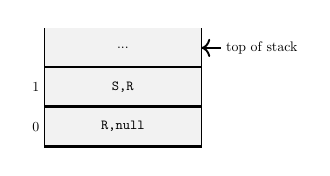
\begin{tikzpicture}[scale=0.5, transform shape]
  \stacktop{} \cellptr{top of stack}
	\separator
	\cell{\texttt{S,R}}        \cellcomL{1} \coordinate () at (currentcell.east);
  \separator
	\cell{\texttt{R,null}}     \cellcomL{0} \coordinate () at (currentcell.east);
  \separator
\end{tikzpicture}
\caption{Operation $op(50)$ starting at R and ending at Z along with the stack}
\end{figure}
\end{frame}
\begin{frame}[c]{Traversal Stack}
\begin{figure}[htp]
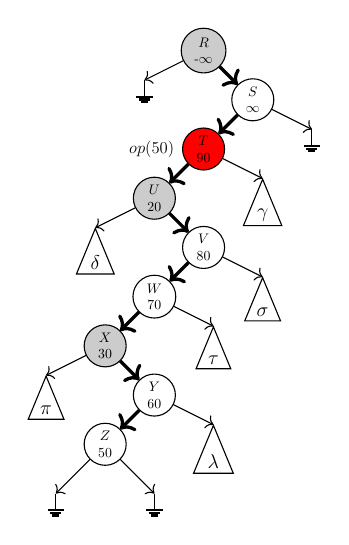
\begin{tikzpicture}[scale=0.5, transform shape] 
	 \newcommand\NODEDX{1.25}
	 \newcommand\NODEDY{1.25}
	 \newcommand\SUBTREEDX{1.5}
	 \newcommand\SUBTREEDY{0.75}
	
   \node (r)	[treenode, fill=black!20] 		at (0, 0)       		                      	{$R$ \\  -$\infty$};
   \node (s)	[treenode] 										at ([shift=({ \NODEDX, -\NODEDY})]r)     	  {$S$ \\  $\infty$};
	 \node (t)	[treenode, fill=red]          at ([shift=({  -\NODEDX, -\NODEDY})]s)    	{$T$ \\ 90};
	 \node (u)	[treenode, fill=black!20] 	  at ([shift=({ -\NODEDX, -\NODEDY})]t)     	{$U$ \\ 20};
	 \node (v)	[treenode] 										at ([shift=({  \NODEDX, -\NODEDY})]u)     	{$V$ \\ 80};
	 \node (w)	[treenode] 										at ([shift=({ -\NODEDX, -\NODEDY})]v)     	{$W$ \\ 70};
	 \node (x)	[treenode, fill=black!20] 		at ([shift=({ -\NODEDX, -\NODEDY})]w)     	{$X$ \\ 30};
	 \node (y)	[treenode] 										at ([shift=({  \NODEDX, -\NODEDY})]x)     	{$Y$ \\ 60};
	 \node (z)	[treenode] 										at ([shift=({ -\NODEDX, -\NODEDY})]y)     	{$Z$ \\ 50};
	 \node (gl) [ground]                      at ([shift=({ -\NODEDX, -\NODEDY})]z)     	{ };
	 \node (gr) [ground]                      at ([shift=({  \NODEDX, -\NODEDY})]z)     	{ };
		
	 \node (sa) [ground]                      at ([shift=({ -\SUBTREEDX, -\SUBTREEDY})]r) { };
	 \node (sb) [ground]                      at ([shift=({ \SUBTREEDX, -\SUBTREEDY})]s) 	{ };
	 \node (sg) [subtree]                     at ([shift=({  \SUBTREEDX, -\SUBTREEDY})]t) {\Large $\gamma$};
	 \node (sd) [subtree]                     at ([shift=({ -\SUBTREEDX, -\SUBTREEDY})]u) {\Large $\delta$};
	 \node (ss) [subtree]                     at ([shift=({  \SUBTREEDX, -\SUBTREEDY})]v) {\Large $\sigma$};
	 \node (st) [subtree]                     at ([shift=({  \SUBTREEDX, -\SUBTREEDY})]w) {\Large $\tau$};
	 \node (sp) [subtree]                     at ([shift=({ -\SUBTREEDX, -\SUBTREEDY})]x) {\Large $\pi$};
	 \node (sl) [subtree]                     at ([shift=({  \SUBTREEDX, -\SUBTREEDY})]y) {\Large $\lambda$};	
	
	 \node (op) [label={left:{\large $op(50)$}}] at ([shift=({-0.5, 0})]t) {};
	
	 \path[every node/.style={font=\sffamily\small}]
	    %(0, 1)  edge[->,very thick]  node {} (r)
		  (r)     edge[->,very thick]  node {} (s)
			(s)     edge[->,very thick]  node {} (t)
			(t)     edge[->,very thick]  node {} (u)
			(u)     edge[->,very thick]  node {} (v)
			(v)     edge[->,very thick]  node {} (w)
			(w)     edge[->,very thick]  node {} (x)
			(x)     edge[->,very thick]  node {} (y)
			(y)     edge[->,very thick]  node {} (z)
			(z)     edge[->]  node {} (gl)
			(z)     edge[->]  node {} (gr)
			(r)     edge[->]  node {} (sa)
			(s)     edge[->]  node {} (sb)
			(t)     edge[->]  node {} (sg.north)
			(u)     edge[->]  node {} (sd.north)
			(v)     edge[->]  node {} (ss.north)
			(w)     edge[->]  node {} (st.north)
			(x)     edge[->]  node {} (sp.north)
			(y)     edge[->]  node {} (sl.north);		
\end{tikzpicture}
%\qquad
%\begin{tikzpicture}[scale=1.0, transform shape]
%\node[stack=9]  {
%0,\nodepart{one}Z,left,6
%\nodepart{two}Y,rigt,6
%\nodepart{three}X,left,3
%\nodepart{four}W,left,3
%\nodepart{five}V,right,3
%\nodepart{six}U,left,1
%\nodepart{seven}T,right,1
%\nodepart{eight}S,right,0
%\nodepart{nine}R,right,-1
%};
%\end{tikzpicture}
\qquad
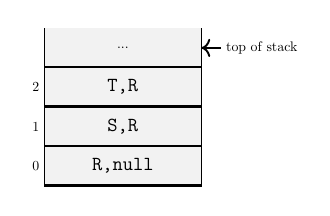
\begin{tikzpicture}[scale=0.5, transform shape]
  \stacktop{} \cellptr{top of stack}
	\separator
	\cell{\Large \texttt{T,R}}        \cellcomL{2} \coordinate () at (currentcell.east);
  \separator
	\cell{\Large \texttt{S,R}}        \cellcomL{1} \coordinate () at (currentcell.east);
  \separator
	\cell{\Large \texttt{R,null}}     \cellcomL{0} \coordinate () at (currentcell.east);
  \separator
\end{tikzpicture}
%\caption{Operation $op(50)$ starting at R and suspended at Y along with the stack}
\end{figure}
\end{frame}


\begin{frame}[c]{Search}
search operations do not restart
\begin{figure}[htp]
\centering
{
	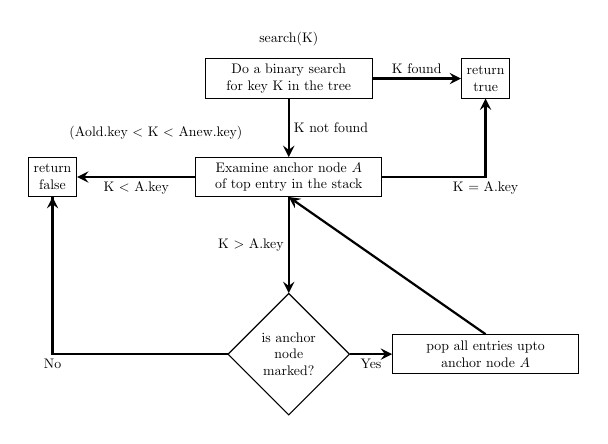
\begin{tikzpicture}[scale=0.5, transform shape]
	\node (p0) [] {search(K)};
	\node (p1) [process, below of=p0, text width=4cm] {Do a binary search for key K in the tree};
	\node (p2) [process, below of=p1, yshift=-1.5cm, text width=4.5cm] {Examine anchor node $A$ of top entry in the stack};
	\node (p3) [decision, below of=p2, yshift=-1.5cm, text width=2cm] {is anchor node marked?};
	\node (p4) [process, right of=p3, xshift=4cm, text width=4.5cm] {pop all entries upto anchor node $A$};
	\node (retT) [process, right of=p1, xshift=4cm, text width=1cm, minimum width=1cm] {return true};
	\node (retF) [process, left of=p2, xshift=-5cm, text width=1cm, minimum width=1cm] {return false};

	\draw [arrow] (p1) -- node[anchor=west] {K not found} (p2);
	\draw [arrow] (p1) -- node[anchor=south] {K found} (retT);
	\draw [arrow] (p2.east) -| node[anchor=north,pos=0.5] {K = A.key}    (retT.south);
	\draw [arrow] (p2.west) -- node (temp) [anchor=north,pos=0.5] {K $<$ A.key}  (retF.east);
	\draw [arrow] (p2) -- node[anchor=east] {K $>$ A.key} (p3);
	\draw [arrow] (p3.west) -| (retF.south) node[below, pos=0.5]{No}  (retF.south);
	\draw [arrow] (p3.east) -- node[anchor=north]{Yes} (p4.west);
	\draw [arrow] (p4.north) -- (p2.south);
	\node (temp1) [above of=temp,xshift=0.5cm,yshift=0.4cm] {(Aold.key $<$ K $<$ Anew.key)};
	\end{tikzpicture}
}
\caption{Sequence of steps in a search operation}
\end{figure}
\end{frame}

\begin{frame}[c]{Search}
\begin{figure}[htp]
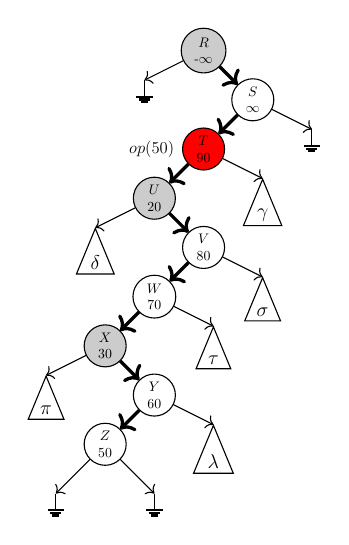
\begin{tikzpicture}[scale=0.5, transform shape] 
	 \newcommand\NODEDX{1.25}
	 \newcommand\NODEDY{1.25}
	 \newcommand\SUBTREEDX{1.5}
	 \newcommand\SUBTREEDY{0.75}
	
   \node (r)	[treenode, fill=black!20] 		at (0, 0)       		                      	{$R$ \\  -$\infty$};
   \node (s)	[treenode] 										at ([shift=({ \NODEDX, -\NODEDY})]r)     	  {$S$ \\  $\infty$};
	 \node (t)	[treenode, fill=red]          at ([shift=({  -\NODEDX, -\NODEDY})]s)    	{$T$ \\ 90};
	 \node (u)	[treenode, fill=black!20] 	  at ([shift=({ -\NODEDX, -\NODEDY})]t)     	{$U$ \\ 20};
	 \node (v)	[treenode] 										at ([shift=({  \NODEDX, -\NODEDY})]u)     	{$V$ \\ 80};
	 \node (w)	[treenode] 										at ([shift=({ -\NODEDX, -\NODEDY})]v)     	{$W$ \\ 70};
	 \node (x)	[treenode, fill=black!20] 		at ([shift=({ -\NODEDX, -\NODEDY})]w)     	{$X$ \\ 30};
	 \node (y)	[treenode] 										at ([shift=({  \NODEDX, -\NODEDY})]x)     	{$Y$ \\ 60};
	 \node (z)	[treenode] 										at ([shift=({ -\NODEDX, -\NODEDY})]y)     	{$Z$ \\ 50};
	 \node (gl) [ground]                      at ([shift=({ -\NODEDX, -\NODEDY})]z)     	{ };
	 \node (gr) [ground]                      at ([shift=({  \NODEDX, -\NODEDY})]z)     	{ };
		
	 \node (sa) [ground]                      at ([shift=({ -\SUBTREEDX, -\SUBTREEDY})]r) { };
	 \node (sb) [ground]                      at ([shift=({ \SUBTREEDX, -\SUBTREEDY})]s) 	{ };
	 \node (sg) [subtree]                     at ([shift=({  \SUBTREEDX, -\SUBTREEDY})]t) {\Large $\gamma$};
	 \node (sd) [subtree]                     at ([shift=({ -\SUBTREEDX, -\SUBTREEDY})]u) {\Large $\delta$};
	 \node (ss) [subtree]                     at ([shift=({  \SUBTREEDX, -\SUBTREEDY})]v) {\Large $\sigma$};
	 \node (st) [subtree]                     at ([shift=({  \SUBTREEDX, -\SUBTREEDY})]w) {\Large $\tau$};
	 \node (sp) [subtree]                     at ([shift=({ -\SUBTREEDX, -\SUBTREEDY})]x) {\Large $\pi$};
	 \node (sl) [subtree]                     at ([shift=({  \SUBTREEDX, -\SUBTREEDY})]y) {\Large $\lambda$};	
	
	 \node (op) [label={left:{\large $op(50)$}}] at ([shift=({-0.5, 0})]t) {};
	
	 \path[every node/.style={font=\sffamily\small}]
	    %(0, 1)  edge[->,very thick]  node {} (r)
		  (r)     edge[->,very thick]  node {} (s)
			(s)     edge[->,very thick]  node {} (t)
			(t)     edge[->,very thick]  node {} (u)
			(u)     edge[->,very thick]  node {} (v)
			(v)     edge[->,very thick]  node {} (w)
			(w)     edge[->,very thick]  node {} (x)
			(x)     edge[->,very thick]  node {} (y)
			(y)     edge[->,very thick]  node {} (z)
			(z)     edge[->]  node {} (gl)
			(z)     edge[->]  node {} (gr)
			(r)     edge[->]  node {} (sa)
			(s)     edge[->]  node {} (sb)
			(t)     edge[->]  node {} (sg.north)
			(u)     edge[->]  node {} (sd.north)
			(v)     edge[->]  node {} (ss.north)
			(w)     edge[->]  node {} (st.north)
			(x)     edge[->]  node {} (sp.north)
			(y)     edge[->]  node {} (sl.north);		
\end{tikzpicture}
%\qquad
%\begin{tikzpicture}[scale=1.0, transform shape]
%\node[stack=9]  {
%0,\nodepart{one}Z,left,6
%\nodepart{two}Y,rigt,6
%\nodepart{three}X,left,3
%\nodepart{four}W,left,3
%\nodepart{five}V,right,3
%\nodepart{six}U,left,1
%\nodepart{seven}T,right,1
%\nodepart{eight}S,right,0
%\nodepart{nine}R,right,-1
%};
%\end{tikzpicture}
\qquad
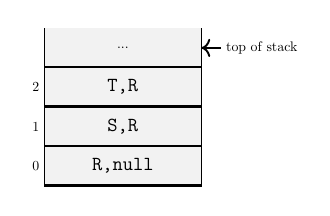
\begin{tikzpicture}[scale=0.5, transform shape]
  \stacktop{} \cellptr{top of stack}
	\separator
	\cell{\Large \texttt{T,R}}        \cellcomL{2} \coordinate () at (currentcell.east);
  \separator
	\cell{\Large \texttt{S,R}}        \cellcomL{1} \coordinate () at (currentcell.east);
  \separator
	\cell{\Large \texttt{R,null}}     \cellcomL{0} \coordinate () at (currentcell.east);
  \separator
\end{tikzpicture}
%\caption{Operation $op(50)$ starting at R and suspended at Y along with the stack}
\end{figure}
\end{frame}
\begin{frame}[c]{Search}
\begin{figure}[htp]
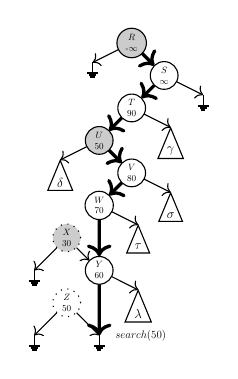
\begin{tikzpicture}[scale=0.33, transform shape]
   
	 \newcommand\NODEDX{1.25}
	 \newcommand\NODEDY{1.25}
	 \newcommand\SUBTREEDX{1.5}
	 \newcommand\SUBTREEDY{0.75}
	
	 \node (r)	[treenode, fill=black!20] 		at (0, 0)       		                      	{$R$ \\  -$\infty$};
   \node (s)	[treenode] 										at ([shift=({ \NODEDX, -\NODEDY})]r)     	  {$S$ \\  $\infty$};
	 \node (t)	[treenode] 		                at ([shift=({  -\NODEDX, -\NODEDY})]s)    	{$T$ \\ 90};
	 \node (u)	[treenode, fill=black!20] 	  at ([shift=({ -\NODEDX, -\NODEDY})]t)     	{$U$ \\ 50};
	 \node (v)	[treenode] 										at ([shift=({  \NODEDX, -\NODEDY})]u)     	{$V$ \\ 80};
	 \node (w)	[treenode] 										at ([shift=({ -\NODEDX, -\NODEDY})]v)     	{$W$ \\ 70};
	 \node (x)	[treenode, fill=black!20, dotted] 		at ([shift=({ -\NODEDX, -\NODEDY})]w)     	{$X$ \\ 30};
	 \node (y)	[treenode] 										at ([shift=({  \NODEDX, -\NODEDY})]x)     	{$Y$ \\ 60};
	 \node (z)	[treenode, dotted] 						at ([shift=({ -\NODEDX, -\NODEDY})]y)     	{$Z$ \\ 50};
	 \node (gl) [ground]                      at ([shift=({ -\NODEDX, -\NODEDY})]z)     	{ };
	 \node (gr) [ground]                      at ([shift=({  \NODEDX, -\NODEDY})]z)     	{ };
		
	 \node (sa) [ground]                      at ([shift=({ -\SUBTREEDX, -\SUBTREEDY})]r) { };
	 \node (sb) [ground]                      at ([shift=({ \SUBTREEDX, -\SUBTREEDY})]s) 	{ };
	 \node (sg) [subtree]                     at ([shift=({  \SUBTREEDX, -\SUBTREEDY})]t) {\Large $\gamma$};
	 \node (sd) [subtree]                     at ([shift=({ -\SUBTREEDX, -\SUBTREEDY})]u) {\Large $\delta$};
	 \node (ss) [subtree]                     at ([shift=({  \SUBTREEDX, -\SUBTREEDY})]v) {\Large $\sigma$};
	 \node (st) [subtree]                     at ([shift=({  \SUBTREEDX, -\SUBTREEDY})]w) {\Large $\tau$};
	 %% \node (sp) [subtree]                     at ([shift=({ -\SUBTREEDX, -\SUBTREEDY})]x) {\Large $\pi$};
	 \node (sp) [ground]                    	at ([shift=({ -\NODEDX, -\NODEDY})]x) { };
	 \node (sl) [subtree]                     at ([shift=({  \SUBTREEDX, -\SUBTREEDY})]y) {\Large $\lambda$};	
	
	 \node (op) [label={right:{\large $search(50)$}}] at ([shift=({0.375, 0})]gr) {};
	
	 \path[every node/.style={font=\sffamily\small}]
	    %(0, 1)  edge[->,very thick]  node {} (r)
		  (r)     edge[->,very thick]  node {} (s)
			(s)     edge[->,very thick]  node {} (t)
			(t)     edge[->,very thick]  node {} (u)
			(u)     edge[->,very thick]  node {} (v)
			(v)     edge[->,very thick]  node {} (w)
			%% (w)     edge[->]  node {} (x)
			(w)     edge[->,very thick]  node {} (y)
			(x)     edge[->]  node {} (y)
			%% (y)     edge[->]  node {} (z)
			(y)     edge[->, very thick]  node {} (gr)
			(z)     edge[->]  node {} (gl)
			(z)     edge[->]  node {} (gr)
			(r)     edge[->]  node {} (sa)
			(s)     edge[->]  node {} (sb)
			(t)     edge[->]  node {} (sg.north)
			(u)     edge[->]  node {} (sd.north)
			(v)     edge[->]  node {} (ss.north)
			(w)     edge[->]  node {} (st.north)
			(x)     edge[->]  node {} (sp)
			(y)     edge[->]  node {} (sl.north);		
\end{tikzpicture}
\quad
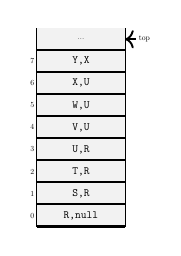
\begin{tikzpicture}[scale=0.28, transform shape]
  \stacktop{} \cellptr{top}
	\separator
	\cell{\Large \texttt{Y,X}}        \cellcomL{7} \coordinate () at (currentcell.east);
  \separator
	\cell{\Large \texttt{X,U}}        \cellcomL{6} \coordinate () at (currentcell.east);
  \separator
	\cell{\Large \texttt{W,U}}        \cellcomL{5} \coordinate () at (currentcell.east);
  \separator
	\cell{\Large \texttt{V,U}}        \cellcomL{4} \coordinate () at (currentcell.east);
  \separator
	\cell{\Large \texttt{U,R}}        \cellcomL{3} \coordinate () at (currentcell.east);
  \separator
	\cell{\Large \texttt{T,R}}        \cellcomL{2} \coordinate () at (currentcell.east);
  \separator
	\cell{\Large \texttt{S,R}}        \cellcomL{1} \coordinate () at (currentcell.east);
  \separator
	\cell{\Large \texttt{R,null}}     \cellcomL{0} \coordinate () at (currentcell.east);
  \separator
\end{tikzpicture}
\quad
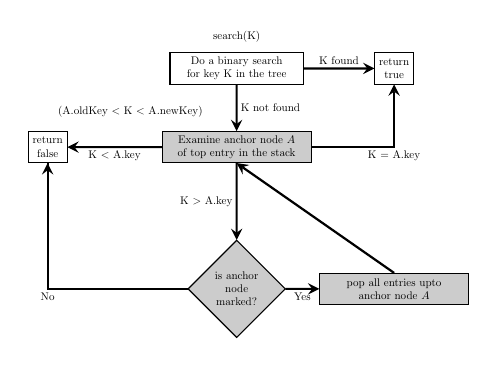
\begin{tikzpicture}[scale=0.4, transform shape]
	\node (p0) [] {search(K)};
	\node (p1) [process, below of=p0, text width=4cm] {Do a binary search for key K in the tree};
	\node (p2) [process, below of=p1, yshift=-1.5cm, text width=4.5cm,fill=black!20] {Examine anchor node $A$ of top entry in the stack};
	\node (p3) [decision, below of=p2, yshift=-1.5cm, text width=2cm,fill=black!20] {is anchor node marked?};
	\node (p4) [process, right of=p3, xshift=4cm, text width=4.5cm,fill=black!20] {pop all entries upto anchor node $A$};
	\node (retT) [process, right of=p1, xshift=4cm, text width=1cm, minimum width=1cm] {return true};
	\node (retF) [process, left of=p2, xshift=-5cm, text width=1cm, minimum width=1cm] {return false};

	\draw [arrow] (p1) -- node[anchor=west] {K not found} (p2);
	\draw [arrow] (p1) -- node[anchor=south] {K found} (retT);
	\draw [arrow] (p2.east) -| node[anchor=north,pos=0.5] {K = A.key}    (retT.south);
	\draw [arrow] (p2.west) -- node (temp) [anchor=north,pos=0.5] {K $<$ A.key}  (retF.east);
	\draw [arrow] (p2) -- node[anchor=east] {K $>$ A.key} (p3);
	\draw [arrow] (p3.west) -| (retF.south) node[below, pos=0.5]{No}  (retF.south);
	\draw [arrow] (p3.east) -- node[anchor=north]{Yes} (p4.west);
	\draw [arrow] (p4.north) -- (p2.south);
	\node (temp1) [above of=temp,xshift=0.5cm,yshift=0.4cm] {(A.oldKey $<$ K $<$ A.newKey)};
	\end{tikzpicture}
\caption{Key 30 is deleted;key 20 is deleted $\&$ replaced with key 50 in node $U$ and node $Z$ is removed}
\end{figure}
\end{frame}
\begin{frame}[c]{Search}
\begin{figure}[htp]
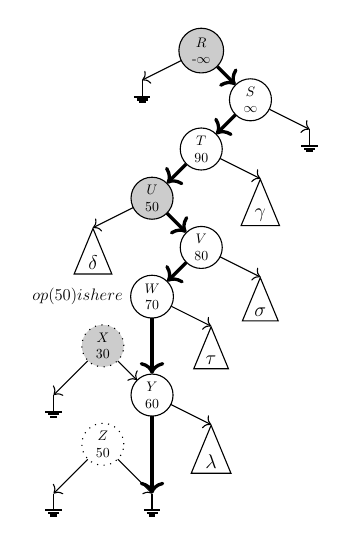
\begin{tikzpicture}[scale=0.5, transform shape]
   
	 \newcommand\NODEDX{1.25}
	 \newcommand\NODEDY{1.25}
	 \newcommand\SUBTREEDX{1.5}
	 \newcommand\SUBTREEDY{0.75}
	
	 \node (r)	[treenode, fill=black!20] 		at (0, 0)       		                      	{$R$ \\  -$\infty$};
   \node (s)	[treenode] 										at ([shift=({ \NODEDX, -\NODEDY})]r)     	  {$S$ \\  $\infty$};
	 \node (t)	[treenode] 		                at ([shift=({  -\NODEDX, -\NODEDY})]s)    	{$T$ \\ 90};
	 \node (u)	[treenode, fill=black!20] 	  at ([shift=({ -\NODEDX, -\NODEDY})]t)     	{$U$ \\ 50};
	 \node (v)	[treenode] 										at ([shift=({  \NODEDX, -\NODEDY})]u)     	{$V$ \\ 80};
	 \node (w)	[treenode] 										at ([shift=({ -\NODEDX, -\NODEDY})]v)     	{$W$ \\ 70};
	 \node (x)	[treenode, fill=black!20, dotted] 		at ([shift=({ -\NODEDX, -\NODEDY})]w)     	{$X$ \\ 30};
	 \node (y)	[treenode] 										at ([shift=({  \NODEDX, -\NODEDY})]x)     	{$Y$ \\ 60};
	 \node (z)	[treenode, dotted] 						at ([shift=({ -\NODEDX, -\NODEDY})]y)     	{$Z$ \\ 50};
	 \node (gl) [ground]                      at ([shift=({ -\NODEDX, -\NODEDY})]z)     	{ };
	 \node (gr) [ground]                      at ([shift=({  \NODEDX, -\NODEDY})]z)     	{ };
		
	 \node (sa) [ground]                      at ([shift=({ -\SUBTREEDX, -\SUBTREEDY})]r) { };
	 \node (sb) [ground]                      at ([shift=({ \SUBTREEDX, -\SUBTREEDY})]s) 	{ };
	 \node (sg) [subtree]                     at ([shift=({  \SUBTREEDX, -\SUBTREEDY})]t) {\Large $\gamma$};
	 \node (sd) [subtree]                     at ([shift=({ -\SUBTREEDX, -\SUBTREEDY})]u) {\Large $\delta$};
	 \node (ss) [subtree]                     at ([shift=({  \SUBTREEDX, -\SUBTREEDY})]v) {\Large $\sigma$};
	 \node (st) [subtree]                     at ([shift=({  \SUBTREEDX, -\SUBTREEDY})]w) {\Large $\tau$};
	 %% \node (sp) [subtree]                     at ([shift=({ -\SUBTREEDX, -\SUBTREEDY})]x) {\Large $\pi$};
	 \node (sp) [ground]                    	at ([shift=({ -\NODEDX, -\NODEDY})]x) { };
	 \node (sl) [subtree]                     at ([shift=({  \SUBTREEDX, -\SUBTREEDY})]y) {\Large $\lambda$};	
	
	 \node (op) [label={left:{\large $op(50) is here$}}] at ([shift=({-0.5, 0})]w) {};
	
	 \path[every node/.style={font=\sffamily\small}]
	    %(0, 1)  edge[->,very thick]  node {} (r)
		  (r)     edge[->,very thick]  node {} (s)
			(s)     edge[->,very thick]  node {} (t)
			(t)     edge[->,very thick]  node {} (u)
			(u)     edge[->,very thick]  node {} (v)
			(v)     edge[->,very thick]  node {} (w)
			%% (w)     edge[->]  node {} (x)
			(w)     edge[->,very thick]  node {} (y)
			(x)     edge[->]  node {} (y)
			%% (y)     edge[->]  node {} (z)
			(y)     edge[->, very thick]  node {} (gr)
			(z)     edge[->]  node {} (gl)
			(z)     edge[->]  node {} (gr)
			(r)     edge[->]  node {} (sa)
			(s)     edge[->]  node {} (sb)
			(t)     edge[->]  node {} (sg.north)
			(u)     edge[->]  node {} (sd.north)
			(v)     edge[->]  node {} (ss.north)
			(w)     edge[->]  node {} (st.north)
			(x)     edge[->]  node {} (sp)
			(y)     edge[->]  node {} (sl.north);		
\end{tikzpicture}
\qquad
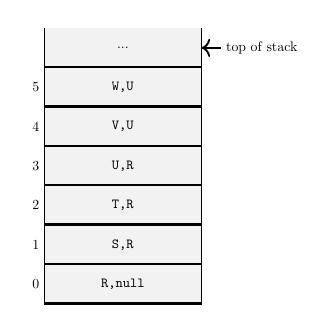
\begin{tikzpicture}[scale=0.5, transform shape]
  \stacktop{} \cellptr{top of stack}
	\separator
	\cell{\texttt{W,U}}        \cellcomL{5} \coordinate () at (currentcell.east);
  \separator
	\cell{\texttt{V,U}}        \cellcomL{4} \coordinate () at (currentcell.east);
  \separator
	\cell{\texttt{U,R}}        \cellcomL{3} \coordinate () at (currentcell.east);
  \separator
	\cell{\texttt{T,R}}        \cellcomL{2} \coordinate () at (currentcell.east);
  \separator
	\cell{\texttt{S,R}}        \cellcomL{1} \coordinate () at (currentcell.east);
  \separator
	\cell{\texttt{R,null}}     \cellcomL{0} \coordinate () at (currentcell.east);
  \separator
\end{tikzpicture}
\caption{Pop upto marked anchor node $X$. Top of stack is now $W$. Examine anchor node $U$}
\end{figure}
\end{frame}

\begin{frame}[c]{Insert}
An insert operation needs to restart only if one of the anchor nodes in the path has become inconsistent
\begin{figure}[htp]
\centering
{
	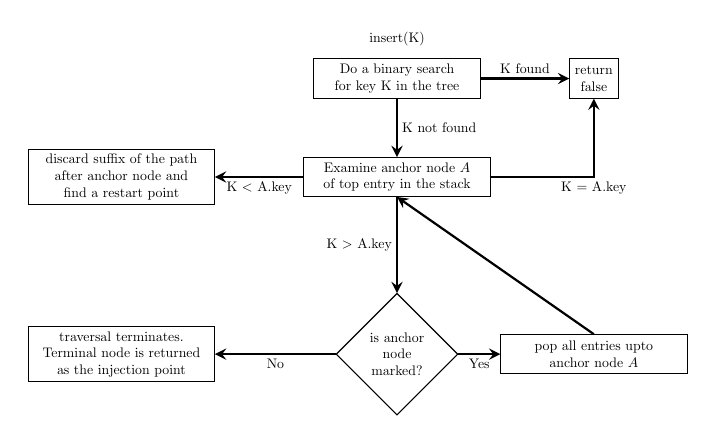
\begin{tikzpicture}[scale=0.5, transform shape]
	\node (p0) [] {insert(K)};
	\node (p1) [process, below of=p0, text width=4cm] {Do a binary search for key K in the tree};
	\node (p2) [process, below of=p1, yshift=-1.5cm, text width=4.5cm] {Examine anchor node $A$ of top entry in the stack};
	\node (p3) [decision, below of=p2, yshift=-1.5cm, text width=2cm] {is anchor node marked?};
	\node (p4) [process, right of=p3, xshift=4cm, text width=4.5cm] {pop all entries upto anchor node $A$};
	\node (retF) [process, right of=p1, xshift=4cm, text width=1cm, minimum width=1cm] {return false};
	\node (retT) [process, left of=p2, xshift=-6cm, text width=4.5cm, minimum width=1cm] {discard suffix of the path after anchor node and find a restart point};
	\node (p5) [process, left of=p3, xshift=-6cm, text width=4.5cm, minimum width=1cm] {traversal terminates. Terminal node is returned as the injection point};

	\draw [arrow] (p1) -- node[anchor=west] {K not found} (p2);
	\draw [arrow] (p1) -- node[anchor=south] {K found} (retF);
	\draw [arrow] (p2.east) -| node[anchor=north,pos=0.5] {K = A.key}    (retF.south);
	\draw [arrow] (p2.west) -- node[anchor=north,pos=0.5] {K $<$ A.key}  (retT.east);
	\draw [arrow] (p2) -- node[anchor=east] {K $>$ A.key} (p3);
	\draw [arrow] (p3.west)  -- node[anchor=north]{No}  (p5.east);
	\draw [arrow] (p3.east) -- node[anchor=north]{Yes} (p4.west);
	\draw [arrow] (p4.north) -- (p2.south);

	\end{tikzpicture}
}
\caption{Sequence of steps in an insert operation}
\end{figure}
\end{frame}

\begin{frame}[c]{Delete}
A delete operation do not restart except when there is a failure in the execution phase
\begin{figure}[htp]
\centering
{
	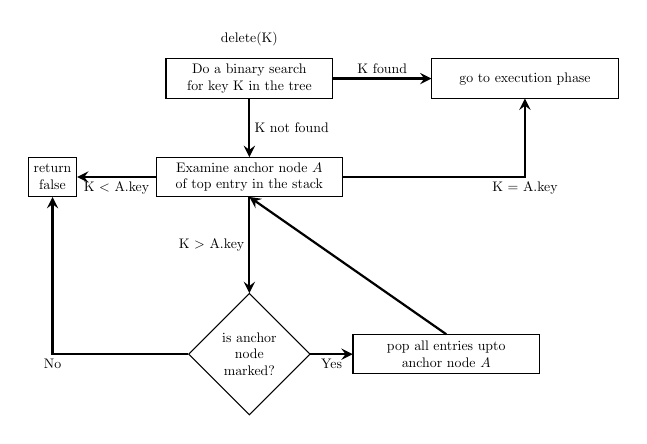
\begin{tikzpicture}[scale=0.5, transform shape]
	\node (p0) [] {delete(K)};
	\node (p1) [process, below of=p0, text width=4cm] {Do a binary search for key K in the tree};
	\node (p2) [process, below of=p1, yshift=-1.5cm, text width=4.5cm] {Examine anchor node $A$ of top entry in the stack};
	\node (p3) [decision, below of=p2, yshift=-1.5cm, text width=2cm] {is anchor node marked?};
	\node (p4) [process, right of=p3, xshift=4cm, text width=4.5cm] {pop all entries upto anchor node $A$};
	\node (ex) [process, right of=p1, xshift=6cm, text width=4.5cm, minimum width=1cm] {go to execution phase};
	\node (retF) [process, left of=p2, xshift=-4cm, text width=1cm, minimum width=1cm] {return false};

	\draw [arrow] (p1) -- node[anchor=west] {K not found} (p2);
	\draw [arrow] (p1) -- node[anchor=south] {K found} (ex);
	\draw [arrow] (p2.east) -| node[anchor=north,pos=0.5] {K = A.key}    (ex.south);
	\draw [arrow] (p2.west) -- node[anchor=north,pos=0.5] {K $<$ A.key}  (retF.east);
	\draw [arrow] (p2) -- node[anchor=east] {K $>$ A.key} (p3);
	\draw [arrow] (p3.west)  -| node[anchor=north]{No}  (retF.south);
	\draw [arrow] (p3.east) -- node[anchor=north]{Yes} (p4.west);
	\draw [arrow] (p4.north) -- (p2.south);

	\end{tikzpicture}
}
\caption{Sequence of steps in a delete operation}
\end{figure}
\end{frame}

\section{Wait free search}
\begin{limitscope}
%%%%% localRecovery/wait free search macros - begin
\newcommand{\remove}[1]{}
\NewDocumentCommand\accesspath{ g g }{\IfNoValueTF{#1}{access-path\xspace}{\IfNoValueTF{#2}{A(#1)\xspace}{A(#1,#2)\xspace}}}
\newcommand{\myterminal}{terminal}
\newcommand{\myanchor}{anchor}
\newcommand{\Myanchor}{Anchor}
\newcommand{\mytarget}{target}
\newcommand{\myadmissible}{admissible}
\newcommand{\mycritical}{critical}
\newcommand{\mysadmissible}{strongly admissible}
\newcommand{\mysafe}{safe}
\newcommand{\myconsistent}{consistent}
\newcommand{\myinconsistent}{inconsistent}
\newcommand{\storedpath}{\Pi}
\newcommand{\prefixpath}[1]{\Pi(#1)}
\newcommand{\injection}{injection}
\newcommand{\myleft}{le\!f\!t}
\newcommand{\myright}{right}
\newcommand{\myparent}{parent}
\newcommand{\InitializeTraversalRecord}{\textsc{InitializeTraversalState}}
\newcommand{\TestForTermination}{\textsc{CanTerminate}}
\newcommand{\FindStartPoint}{\textsc{FindASafeNode}}
\newcommand{\FindAdmissible}{\textsc{ValidatePath}}
\newcommand{\RemoveFromTop}{\textsc{RemoveFromTop}}
\newcommand{\AddToTop}{\textsc{AddToTop}}
\newcommand{\GetTop}{\textsc{GetTop}}
\newcommand{\GetSecondToTop}{\textsc{GetSecondToTop}}
\newcommand{\RemoveUntilCritical}{\textsc{RemoveUntil}}
\newcommand{\RememberCritical}{\textsc{RememberCritical}}
\newcommand{\GetFullEntry}{\textsc{GetFullEntry}}
\newcommand{\IsMarked}{\textsc{IsMarked}}
\newcommand{\IsClean}{\textsc{IsClean}}
\newcommand{\NeedCleanParentNode}{\textsc{NeedCleanParentNode}}
\newcommand{\AddToBottom}{\textsc{AddToBottom}}
\newcommand{\MoveFromTargetToSuccessor}{\textsc{MoveFromTargetToSuccessor}}
\newcommand{\IsEmpty}{\textsc{IsEmpty}}
\newcommand{\Size}{\textsc{Size}}
\newcommand{\GetKey}{\textsc{GetKey}}
\newcommand{\SeekForSuccessor}{\textsc{SeekForSuccessor}}
\newcommand{\NeedSuccessorKey}{\textsc{NeedSuccessorKey}}
\newcommand{\GetChild}{\textsc{GetChild}}
\newcommand{\Move}{\textsc{Move}}
\newcommand{\GetAddress}{\textsc{GetAddress}}
\newcommand{\IsNull}{\textsc{IsNull}}
\newcommand{\PopulateSeekRecord}{\textsc{PopulateSeekRecord}}
\newcommand{\SeekForModify}{\textsc{SeekForModify}}
\newcommand{\SeekForSearch}{\textsc{SeekForSearch}}
\newcommand{\TraverseTree}{\textsc{Traverse}}
\newcommand{\ExamineStack}{\textsc{ExamineStack}}
\newcommand{\numberOfProcesses}{p}
\newcommand{\STELLAR}{\textsc{STELLAR}}
\newcommand{\sNodeOne}{\mathbb{R}}
\newcommand{\sNodeTwo}{\mathbb{S}}
\newcommand{\sKeyOne}{-\infty}
\newcommand{\sKeyTwo}{\infty}
\newcommand{\traversalRecord}{state}
\newcommand{\TraversalRecord}{\textsf{State}}
\newcommand{\opRecord}{opRecord}
\newcommand{\OpRecord}{\textsf{OpRecord}}
\newcommand{\seekRecord}{seekRecord}
\newcommand{\SeekRecord}{\textsf{SeekRecord}}
\newcommand{\maximumgap}{49\%}
\newcommand{\maximumdrop}{10\%}
\newcommand{\dCounters}{DC}
\newcommand{\iCounters}{IC}
\newcommand{\labels}{labels}
\newcommand{\dcounters}{DC}
\newcommand{\icounters}{IC}
\newcommand{\myfigurescaletwo}{0.5}
%%%%% localRecovery/wait free search macros - end
In this chapter we present two light-weight techniques to make search operations for concurrent binary search trees based on internal representation, \emph{wait-free} with low additional overhead. Both of our techniques have the desirable feature that a search operation does not need to perform any write instructions on the share memory thereby minimizing the cache coherence traffic.

\begin{limitscope}
%%%%% localRecovery/wait free search macros - begin
\newcommand{\remove}[1]{}
\NewDocumentCommand\accesspath{ g g }{\IfNoValueTF{#1}{access-path\xspace}{\IfNoValueTF{#2}{A(#1)\xspace}{A(#1,#2)\xspace}}}
\newcommand{\myterminal}{terminal}
\newcommand{\myanchor}{anchor}
\newcommand{\Myanchor}{Anchor}
\newcommand{\mytarget}{target}
\newcommand{\myadmissible}{admissible}
\newcommand{\mycritical}{critical}
\newcommand{\mysadmissible}{strongly admissible}
\newcommand{\mysafe}{safe}
\newcommand{\myconsistent}{consistent}
\newcommand{\myinconsistent}{inconsistent}
\newcommand{\storedpath}{\Pi}
\newcommand{\prefixpath}[1]{\Pi(#1)}
\newcommand{\injection}{injection}
\newcommand{\myleft}{le\!f\!t}
\newcommand{\myright}{right}
\newcommand{\myparent}{parent}
\newcommand{\InitializeTraversalRecord}{\textsc{InitializeTraversalState}}
\newcommand{\TestForTermination}{\textsc{CanTerminate}}
\newcommand{\FindStartPoint}{\textsc{FindASafeNode}}
\newcommand{\FindAdmissible}{\textsc{ValidatePath}}
\newcommand{\RemoveFromTop}{\textsc{RemoveFromTop}}
\newcommand{\AddToTop}{\textsc{AddToTop}}
\newcommand{\GetTop}{\textsc{GetTop}}
\newcommand{\GetSecondToTop}{\textsc{GetSecondToTop}}
\newcommand{\RemoveUntilCritical}{\textsc{RemoveUntil}}
\newcommand{\RememberCritical}{\textsc{RememberCritical}}
\newcommand{\GetFullEntry}{\textsc{GetFullEntry}}
\newcommand{\IsMarked}{\textsc{IsMarked}}
\newcommand{\IsClean}{\textsc{IsClean}}
\newcommand{\NeedCleanParentNode}{\textsc{NeedCleanParentNode}}
\newcommand{\AddToBottom}{\textsc{AddToBottom}}
\newcommand{\MoveFromTargetToSuccessor}{\textsc{MoveFromTargetToSuccessor}}
\newcommand{\IsEmpty}{\textsc{IsEmpty}}
\newcommand{\Size}{\textsc{Size}}
\newcommand{\GetKey}{\textsc{GetKey}}
\newcommand{\SeekForSuccessor}{\textsc{SeekForSuccessor}}
\newcommand{\NeedSuccessorKey}{\textsc{NeedSuccessorKey}}
\newcommand{\GetChild}{\textsc{GetChild}}
\newcommand{\Move}{\textsc{Move}}
\newcommand{\GetAddress}{\textsc{GetAddress}}
\newcommand{\IsNull}{\textsc{IsNull}}
\newcommand{\PopulateSeekRecord}{\textsc{PopulateSeekRecord}}
\newcommand{\SeekForModify}{\textsc{SeekForModify}}
\newcommand{\SeekForSearch}{\textsc{SeekForSearch}}
\newcommand{\TraverseTree}{\textsc{Traverse}}
\newcommand{\ExamineStack}{\textsc{ExamineStack}}
\newcommand{\numberOfProcesses}{p}
\newcommand{\STELLAR}{\textsc{STELLAR}}
\newcommand{\sNodeOne}{\mathbb{R}}
\newcommand{\sNodeTwo}{\mathbb{S}}
\newcommand{\sKeyOne}{-\infty}
\newcommand{\sKeyTwo}{\infty}
\newcommand{\traversalRecord}{state}
\newcommand{\TraversalRecord}{\textsf{State}}
\newcommand{\opRecord}{opRecord}
\newcommand{\OpRecord}{\textsf{OpRecord}}
\newcommand{\seekRecord}{seekRecord}
\newcommand{\SeekRecord}{\textsf{SeekRecord}}
\newcommand{\maximumgap}{49\%}
\newcommand{\maximumdrop}{10\%}
\newcommand{\dCounters}{DC}
\newcommand{\iCounters}{IC}
\newcommand{\labels}{labels}
\newcommand{\dcounters}{DC}
\newcommand{\icounters}{IC}
\newcommand{\myfigurescaletwo}{0.5}
%%%%% localRecovery/wait free search macros - end
In this chapter we present two light-weight techniques to make search operations for concurrent binary search trees based on internal representation, \emph{wait-free} with low additional overhead. Both of our techniques have the desirable feature that a search operation does not need to perform any write instructions on the share memory thereby minimizing the cache coherence traffic.

\begin{limitscope}
%%%%% localRecovery/wait free search macros - begin
\newcommand{\remove}[1]{}
\NewDocumentCommand\accesspath{ g g }{\IfNoValueTF{#1}{access-path\xspace}{\IfNoValueTF{#2}{A(#1)\xspace}{A(#1,#2)\xspace}}}
\newcommand{\myterminal}{terminal}
\newcommand{\myanchor}{anchor}
\newcommand{\Myanchor}{Anchor}
\newcommand{\mytarget}{target}
\newcommand{\myadmissible}{admissible}
\newcommand{\mycritical}{critical}
\newcommand{\mysadmissible}{strongly admissible}
\newcommand{\mysafe}{safe}
\newcommand{\myconsistent}{consistent}
\newcommand{\myinconsistent}{inconsistent}
\newcommand{\storedpath}{\Pi}
\newcommand{\prefixpath}[1]{\Pi(#1)}
\newcommand{\injection}{injection}
\newcommand{\myleft}{le\!f\!t}
\newcommand{\myright}{right}
\newcommand{\myparent}{parent}
\newcommand{\InitializeTraversalRecord}{\textsc{InitializeTraversalState}}
\newcommand{\TestForTermination}{\textsc{CanTerminate}}
\newcommand{\FindStartPoint}{\textsc{FindASafeNode}}
\newcommand{\FindAdmissible}{\textsc{ValidatePath}}
\newcommand{\RemoveFromTop}{\textsc{RemoveFromTop}}
\newcommand{\AddToTop}{\textsc{AddToTop}}
\newcommand{\GetTop}{\textsc{GetTop}}
\newcommand{\GetSecondToTop}{\textsc{GetSecondToTop}}
\newcommand{\RemoveUntilCritical}{\textsc{RemoveUntil}}
\newcommand{\RememberCritical}{\textsc{RememberCritical}}
\newcommand{\GetFullEntry}{\textsc{GetFullEntry}}
\newcommand{\IsMarked}{\textsc{IsMarked}}
\newcommand{\IsClean}{\textsc{IsClean}}
\newcommand{\NeedCleanParentNode}{\textsc{NeedCleanParentNode}}
\newcommand{\AddToBottom}{\textsc{AddToBottom}}
\newcommand{\MoveFromTargetToSuccessor}{\textsc{MoveFromTargetToSuccessor}}
\newcommand{\IsEmpty}{\textsc{IsEmpty}}
\newcommand{\Size}{\textsc{Size}}
\newcommand{\GetKey}{\textsc{GetKey}}
\newcommand{\SeekForSuccessor}{\textsc{SeekForSuccessor}}
\newcommand{\NeedSuccessorKey}{\textsc{NeedSuccessorKey}}
\newcommand{\GetChild}{\textsc{GetChild}}
\newcommand{\Move}{\textsc{Move}}
\newcommand{\GetAddress}{\textsc{GetAddress}}
\newcommand{\IsNull}{\textsc{IsNull}}
\newcommand{\PopulateSeekRecord}{\textsc{PopulateSeekRecord}}
\newcommand{\SeekForModify}{\textsc{SeekForModify}}
\newcommand{\SeekForSearch}{\textsc{SeekForSearch}}
\newcommand{\TraverseTree}{\textsc{Traverse}}
\newcommand{\ExamineStack}{\textsc{ExamineStack}}
\newcommand{\numberOfProcesses}{p}
\newcommand{\STELLAR}{\textsc{STELLAR}}
\newcommand{\sNodeOne}{\mathbb{R}}
\newcommand{\sNodeTwo}{\mathbb{S}}
\newcommand{\sKeyOne}{-\infty}
\newcommand{\sKeyTwo}{\infty}
\newcommand{\traversalRecord}{state}
\newcommand{\TraversalRecord}{\textsf{State}}
\newcommand{\opRecord}{opRecord}
\newcommand{\OpRecord}{\textsf{OpRecord}}
\newcommand{\seekRecord}{seekRecord}
\newcommand{\SeekRecord}{\textsf{SeekRecord}}
\newcommand{\maximumgap}{49\%}
\newcommand{\maximumdrop}{10\%}
\newcommand{\dCounters}{DC}
\newcommand{\iCounters}{IC}
\newcommand{\labels}{labels}
\newcommand{\dcounters}{DC}
\newcommand{\icounters}{IC}
\newcommand{\myfigurescaletwo}{0.5}
%%%%% localRecovery/wait free search macros - end
In this chapter we present two light-weight techniques to make search operations for concurrent binary search trees based on internal representation, \emph{wait-free} with low additional overhead. Both of our techniques have the desirable feature that a search operation does not need to perform any write instructions on the share memory thereby minimizing the cache coherence traffic.

\input{Figures/waitFreeSearch}
The search operations in~\cite{HowJon:2012:SPAA,DraVec+:2014:PPoPP,ArbAtt:2014:PODC,RamMit:2015:ICDCN,RamMit:2015:PPoPP} are \emph{not wait-free} even for a bounded key space. For example, in \figref{waitFreeSearch} thread $A$ executes \textsf{contains(15)} and thread $B$ executes a series of operations preventing the \textsf{contains} operation of thread $A$ to terminate. Note that the tree in (a) and (e) are same and this sequence of operations can occur ad infinitum. Hence the search operation is not wait-free.

In our first approach, we keep track of the count of modify operations. Here we do not make any new modifications to the tree node. In our second approach, we append a timestamp to the tree node but it has better complexity than the previous one.

\section{No Modification to Tree Node}
Due to the limited manner in which the tree can evolve in the concurrent algorithms described in~\cite{HowJon:2012:SPAA,DraVec+:2014:PPoPP,ArbAtt:2014:PODC,RamMit:2015:ICDCN,RamMit:2015:PPoPP}, it is possible to design a light-weight wait-free algorithm for a search operation for all of the algorithms. The main property we use is that as long as a key is \emph{continuously} present in the tree, its distance from the root of the tree is \emph{monotonically non-increasing}. As a result, if a key is not found after visiting a ``certain'' number of nodes in the tree, then the traversal can stop and it is sufficient to examine the path traversed to check whether or not the key has moved up. In case the key is not continuously present in the tree, while a search operation is in progress, it is acceptable to return either of the 
outcomes---present or not present---to the application. In the first case, the search operation can be linearized after the insert operation that added the key to the tree. In the second case, it can be linearized after the delete operation that removed the key from the tree. 

The main question is: ``How do we \emph{efficiently} determine the number of nodes to visit in the tree before stopping the downward traversal \emph{without missing} the key that is continuously present in the tree?'' To that end, we maintain two arrays with one entry for each process in the array, denoted by $\iCounters$ and $\dCounters$. Roughly speaking, entries $\iCounters[i]$ and $\dCounters[i]$ denote the number of insert and delete operations, respectively, process $P_i$ has performed so far. A process increments its insert counter before adding a key to the tree and its delete counter after removing a key from the tree. As a result, the insert (delete) counter at a process is an upper (lower) bound on the number of keys that the process has added to (removed from) the tree. Before starting downward traversal for a search operation, a process first reads the delete counter values of all processes and then reads the insert counter values of all processes. It then computes an estimate for the number of nodes to visit as the sum of all the insert counter values minus the sum of all the delete counter values. We show that the estimate computed by a process is \emph{safe} in the sense that a search operation will not miss a key continuously present in the tree while the operation is in progress.

To show that our algorithm works, we introduce some notation. Consider a time $t$ \emph{after} an operation has read all the delete counter values but \emph{before} its starts reading any of the insert counter values. Let $I_{t,i}$ ($D_{t,i}$) denote the \emph{actual} number of keys added to (removed from) the tree by process $P_i$ at or before time $t$. Also, let $\icounters[i]$ ($\dcounters[i]$) denote the value read for $\iCounters[i]$ ($\dCounters[i]$) by the operation. Note that, the way counters are maintained, $\icounters[i] \geq I_{t,i}$ and $\dcounters[i] \leq D_{t,i}$. Also, let $S_t$ and $\Delta_t$ denote the \emph{actual} size of the tree and the \emph{actual} distance of the target key from the root of the tree, respectively, at time $t$. Clearly, we have:
%%
\[
S_t = \sum_{0 \leq i < \numberOfProcesses} I_{t,i} - \sum_{0 \leq i < \numberOfProcesses} D_{t,i} \text{\quad and \quad} \Delta_t \leq S_t
\]
%%
Thus we have:
\[
\sum_{0 \leq i < \numberOfProcesses} \icounters[i] - \sum_{0 \leq i < \numberOfProcesses} \dcounters[i]  \; \geq \; \sum_{0 \leq i < \numberOfProcesses} I_{t,i} - \sum_{0 \leq i < \numberOfProcesses} D_{t,i} \; = \; S_t 
\]
%%
In other words, the estimate computed by our algorithm is an upper bound on the actual distance of the key from the root of tree when the operation starts traversing the tree (which is monotonically non-increasing).

A pseudo-code of the algorithm is given in \pseudoref{wf:search:size}. In the pseudo-code, $\numberOfProcesses$ denotes the number of processes. To amortize the overhead of reading $O(\numberOfProcesses)$ counters, an operation first visits $\numberOfProcesses$ nodes in the tree. If it does not find the key, then it reads the counter values and proceeds as described above. Thus $O(\numberOfProcesses)$ overhead is incurred only for ``large'' trees.

Some advantages of our approach are as follows. First, it works even if a key space is unbounded. Second, it does not require a search operation to perform any write instruction on shared memory. Third, it does not require a modify operation to perform any additional atomic instruction or helping (besides that performed by the original algorithm). 

\input{waitFreeSearch/pseudocode-waitfree}

\section{With Modification to Tree Node}
A disadvantage of the previous approach is that the time complexity of a search operation depends on the tree size. We now describe another approach to achieve wait-freedom for which the time complexity of a search operation depends on the tree height. This approach, however, requires modifying tree node to store a time-stamp of when the node was created. It consists of the identifier of the process that created the node and the process-specific sequence number (which is incremented before the node is added to the tree). This time-stamp is copied if a node is \emph{replaced} with a new node (in a complex delete operation) as in~\cite{RamMit:2015:ICDCN}. Before a search operation starts traversing the tree, it reads the current sequence number values of all processes. Let $\labels[i]$ denote the value read for process $P_i$. The operation then stops the downward traversal of the tree once it encounters a node with time-stamp $\ang{i,v}$ such that $v > \labels[i]$. Clearly, this node and its descendants were added to the tree after the operation read the sequence number value of process $P_i$.
%%
A pseudo-code of the algorithm is given in \pseudoref{wf:search:height}.
\end{limitscope}
The search operations in~\cite{HowJon:2012:SPAA,DraVec+:2014:PPoPP,ArbAtt:2014:PODC,RamMit:2015:ICDCN,RamMit:2015:PPoPP} are \emph{not wait-free} even for a bounded key space. For example, in \figref{waitFreeSearch} thread $A$ executes \textsf{contains(15)} and thread $B$ executes a series of operations preventing the \textsf{contains} operation of thread $A$ to terminate. Note that the tree in (a) and (e) are same and this sequence of operations can occur ad infinitum. Hence the search operation is not wait-free.

In our first approach, we keep track of the count of modify operations. Here we do not make any new modifications to the tree node. In our second approach, we append a timestamp to the tree node but it has better complexity than the previous one.

\section{No Modification to Tree Node}
Due to the limited manner in which the tree can evolve in the concurrent algorithms described in~\cite{HowJon:2012:SPAA,DraVec+:2014:PPoPP,ArbAtt:2014:PODC,RamMit:2015:ICDCN,RamMit:2015:PPoPP}, it is possible to design a light-weight wait-free algorithm for a search operation for all of the algorithms. The main property we use is that as long as a key is \emph{continuously} present in the tree, its distance from the root of the tree is \emph{monotonically non-increasing}. As a result, if a key is not found after visiting a ``certain'' number of nodes in the tree, then the traversal can stop and it is sufficient to examine the path traversed to check whether or not the key has moved up. In case the key is not continuously present in the tree, while a search operation is in progress, it is acceptable to return either of the 
outcomes---present or not present---to the application. In the first case, the search operation can be linearized after the insert operation that added the key to the tree. In the second case, it can be linearized after the delete operation that removed the key from the tree. 

The main question is: ``How do we \emph{efficiently} determine the number of nodes to visit in the tree before stopping the downward traversal \emph{without missing} the key that is continuously present in the tree?'' To that end, we maintain two arrays with one entry for each process in the array, denoted by $\iCounters$ and $\dCounters$. Roughly speaking, entries $\iCounters[i]$ and $\dCounters[i]$ denote the number of insert and delete operations, respectively, process $P_i$ has performed so far. A process increments its insert counter before adding a key to the tree and its delete counter after removing a key from the tree. As a result, the insert (delete) counter at a process is an upper (lower) bound on the number of keys that the process has added to (removed from) the tree. Before starting downward traversal for a search operation, a process first reads the delete counter values of all processes and then reads the insert counter values of all processes. It then computes an estimate for the number of nodes to visit as the sum of all the insert counter values minus the sum of all the delete counter values. We show that the estimate computed by a process is \emph{safe} in the sense that a search operation will not miss a key continuously present in the tree while the operation is in progress.

To show that our algorithm works, we introduce some notation. Consider a time $t$ \emph{after} an operation has read all the delete counter values but \emph{before} its starts reading any of the insert counter values. Let $I_{t,i}$ ($D_{t,i}$) denote the \emph{actual} number of keys added to (removed from) the tree by process $P_i$ at or before time $t$. Also, let $\icounters[i]$ ($\dcounters[i]$) denote the value read for $\iCounters[i]$ ($\dCounters[i]$) by the operation. Note that, the way counters are maintained, $\icounters[i] \geq I_{t,i}$ and $\dcounters[i] \leq D_{t,i}$. Also, let $S_t$ and $\Delta_t$ denote the \emph{actual} size of the tree and the \emph{actual} distance of the target key from the root of the tree, respectively, at time $t$. Clearly, we have:
%%
\[
S_t = \sum_{0 \leq i < \numberOfProcesses} I_{t,i} - \sum_{0 \leq i < \numberOfProcesses} D_{t,i} \text{\quad and \quad} \Delta_t \leq S_t
\]
%%
Thus we have:
\[
\sum_{0 \leq i < \numberOfProcesses} \icounters[i] - \sum_{0 \leq i < \numberOfProcesses} \dcounters[i]  \; \geq \; \sum_{0 \leq i < \numberOfProcesses} I_{t,i} - \sum_{0 \leq i < \numberOfProcesses} D_{t,i} \; = \; S_t 
\]
%%
In other words, the estimate computed by our algorithm is an upper bound on the actual distance of the key from the root of tree when the operation starts traversing the tree (which is monotonically non-increasing).

A pseudo-code of the algorithm is given in \pseudoref{wf:search:size}. In the pseudo-code, $\numberOfProcesses$ denotes the number of processes. To amortize the overhead of reading $O(\numberOfProcesses)$ counters, an operation first visits $\numberOfProcesses$ nodes in the tree. If it does not find the key, then it reads the counter values and proceeds as described above. Thus $O(\numberOfProcesses)$ overhead is incurred only for ``large'' trees.

Some advantages of our approach are as follows. First, it works even if a key space is unbounded. Second, it does not require a search operation to perform any write instruction on shared memory. Third, it does not require a modify operation to perform any additional atomic instruction or helping (besides that performed by the original algorithm). 

\begin{limitscope}

%% To limit the scope of the macros defined below

%% macros for pseudocode

\newcommand{\child}{child}
\newcommand{\node}{node}
\newcommand{\parent}{parent}

\newcommand{\mainSeekRecord}{seekTargetKey}
\newcommand{\successorSeekRecord}{seekSuccessorKey}


\newcommand{\targetStack}{targetStack}
\newcommand{\successorStack}{successorStack}


\newcommand{\successorStackInUse}{successorStackInUse}
\newcommand{\targetNode}{targetNode}




\newcommand{\key}{key}

\newcommand{\done}{done}
\newcommand{\result}{result}
\newcommand{\status}{status}
\newcommand{\restart}{restart}





\newcommand{\cKey}{key}
\newcommand{\nKey}{key}
\newcommand{\cNode}{current}
\newcommand{\pNode}{parent}
\newcommand{\nMarked}{marked}



\newcommand{\which}{which}
\newcommand{\address}{address}

\newcommand{\anchor}{anchor}

\newcommand{\stack}{stack}
\newcommand{\sTop}{top}
\newcommand{\sBottom}{bottom}
\newcommand{\current}{current}

\remove{
\newcommand{\traversalRecord}{state}
\newcommand{\TraversalRecord}{State}
\newcommand{\opRecord}{opRecord}
\newcommand{\OpRecord}{OpRecord}
\newcommand{\seekRecord}{seekRecord}
\newcommand{\SeekRecord}{SeekRecord}
}

\newcommand{\admissible}{admissible}
\newcommand{\critical}{critical}
\newcommand{\reference}{re\!f\!erence}

\newcommand{\OptReturn}[1][]{\Return #1\;}

\newcommand{\injectionPoint}{injectionPoint}



\newcommand{\Search}{\textsc{Search}}
\newcommand{\Insert}{\textsc{Insert}}
\newcommand{\Delete}{\textsc{Delete}}
\newcommand{\Seek}{\textsc{Seek}}

\newcommand{\Inject}{\textsc{Inject}}


%%
%% \newcommand{\WFSeekForSearchBOSize}{\textsc{WFSeekForSearchBasedOnSize}}
\newcommand{\WFSeekForSearchBOSize}{\textsc{WFSeekForSearchBOSize}}
%% \newcommand{\WFSeekForSearchBOHeight}{\textsc{WFSeekForSearchBasedOnHeight}}
\newcommand{\WFSeekForSearchBOHeight}{\textsc{WFSeekForSearchBOHeight}}
%%
%% \newcommand{\WFTraverseTreeBOCount}{\textsc{TraverseBasedOnCount}}
\newcommand{\WFTraverseTreeBOCount}{\textsc{LimitedSeek}}
%% \newcommand{\WFTraverseTreeBOTimeStamp}{\textsc{TraverseBasedOnTimeStamp}}
\newcommand{\WFTraverseTreeBOTimeStamp}{\textsc{TimeStampSeek}}
%%
\remove{
\newcommand{\SeekForSuccessor}{\textsc{SeekForSuccessor}}
\newcommand{\NeedSuccessorKey}{\textsc{NeedSuccessorKey}}
\newcommand{\GetChild}{\textsc{GetChild}}
\newcommand{\Move}{\textsc{Move}}
\newcommand{\GetAddress}{\textsc{GetAddress}}
\newcommand{\IsNull}{\textsc{IsNull}}
\newcommand{\PopulateSeekRecord}{\textsc{PopulateSeekRecord}}
}

%%


\newcommand{\dSum}{\mathcal{D}}
\newcommand{\iSum}{\mathcal{I}}

\newcommand{\copyOfLabels}{copyO\!f\!Labels}
\newcommand{\timeStamp}{timeStamp}
\newcommand{\myLabel}{label}
\newcommand{\myPID}{pid}

\newcommand{\mline}[1]{\DontPrintSemicolon #1 \PrintSemicolon}


\newcommand{\LEFT}{\textsf{LEFT}}
\newcommand{\RIGHT}{\textsf{RIGHT}}


\newcommand{\rarrow}{\!\rightarrow\!}
\newcommand{\type}{type}
\newcommand{\limit}{limit}


\newcommand{\SEARCH}{\textsf{SEARCH}}
\newcommand{\INSERT}{\textsf{INSERT}}
\newcommand{\DELETE}{\textsf{DELETE}}

\newcommand{\STOPFOUND}{\textsf{FOUND}}
\newcommand{\STOPNOTFOUND}{\textsf{NOT\_FOUND}}
\newcommand{\ADMISSIBLE}{\textsf{SAFE}}
\newcommand{\INADMISSIBLE}{\textsf{NOT\_SAFE}}

\newcommand{\TARGETSTACK}{\textsf{TARGET\_STACK}}
\newcommand{\SUCCESSORSTACK}{\textsf{SUCCESSOR\_STACK}}

%%%%%%%%%%%%%%%%%%%%%%%%%%%%%%%%%%%%%%%%%%%%%%%%%%%%%%%%%%%%%%%%%%%%%%%%%%%%%%%%%%%%

\newcommand{\DefineKeyWords}{
%%
\SetKw{Boolean}{boolean}
\SetKw{Integer}{integer}
\SetKw{LAnd}{~and~}
\SetKw{LOr}{~or~}
\SetKw{LNot}{not}
\SetKw{Struct}{struct}
\SetKw{Null}{null}
\SetKw{True}{true}
\SetKw{False}{false}
\SetKw{Break}{break}
\SetKw{Continue}{continue}
\SetKw{Enum}{enum}
\SetKw{Word}{word}
%%
}

%%%%%%%%%%%%%%%%%%%%%%%%%%%%%%%%%%%%%%%%%%%%%%%%%%%%%%%%%%%%%%%%%%%%%%%%%%%%%%%%%%%%%

%% Functions for wait-free search

%%%%%%%%%%%%%%%%%%%%%%%%%%%%%%%%%%%%%%%%%%%%%%%%%%%%%%%%%%%%%%%%%%%%%%%%%%%%%%%%%%%%%




\begin{algorithm}[htp]
\caption{Seek Function for Target Key based on Estimating Tree Size} 
\label{algo:wf:search:size}
%%
\DefineKeyWords
%%
\Integer $\iCounters[\numberOfProcesses]$\;
\Integer $\dCounters[\numberOfProcesses]$\;
%%
\BlankLine
%%
\tcp{Traverses the tree starting from the root node but visits a limited number of nodes}
\DontPrintSemicolon
\Boolean \WFTraverseTreeBOCount( $\opRecord$, $\seekRecord$, $\limit$ )\;
%% \Boolean \WFTraverseTreeBOCount( $\opRecord$,  $\limit$ )\;
\PrintSemicolon
\Begin
{
%%
\tcp{similar to \TraverseTree{} except that the while loop from \linesref{local-seek:while:traversal:begin}{local-seek:while:traversal:end} is executed at most $\limit$ times}
%%
}
%%
\BlankLine
%%
\tcp{A wait-free seek function for a search operation based on computing an upper-bound on tree size}
\DontPrintSemicolon
\Boolean \WFSeekForSearchBOSize( $\opRecord$, $\seekRecord$ )\;
\PrintSemicolon
\Begin
{
%%
   %% $\limit$ := $\numberOfProcesses$\;
	 $\result$ := \WFTraverseTreeBOCount(  $\opRecord$, $\seekRecord$, $\numberOfProcesses$ )\;
	 \If{\LNot($\result$)} 
	 {
	    %% $\dSum$ := $\sum\limits_{i = 0}^{\numberOfProcesses-1}  \dCounters[i]$\;
			%% $\iSum$ := $\sum\limits_{i = 0}^{\numberOfProcesses-1}  \iCounters[i]$\;
			$\dSum$ := $\dCounters[0] + \dCounters[1] + \cdots + \dCounters[\numberOfProcesses-1]$\;
		  $\iSum$ := $\iCounters[0] + \iCounters[1] + \cdots + \iCounters[\numberOfProcesses-1]$\;
			$S$ := $\iSum - \dSum$\;
			$\result$ :=  \WFTraverseTreeBOCount(  $\opRecord$, $\seekRecord$, $S$ )\;
			
	 }
	 
	 \If{\LNot($\result$)}
	 {
	    \tcp{examine the stack}
			$\result$ := \ExamineStack( $\opRecord$, $\seekRecord$ )\;
	 }
	 
	 \tcp{return the outcome}
	 %% \tcp{return the outcome}
	 \PopulateSeekRecord( $\seekRecord$, $\traversalRecord$ )\;
	 \Return $\result$\;
	
%%
}
\end{algorithm}




\begin{algorithm}[htp]
\caption{Seek Function for Target Key based on Time-Stamps} 
\label{algo:wf:search:height}
%%
\DefineKeyWords
%%
\Integer $\labels[\numberOfProcesses]$\;
%%
\BlankLine
%%
\tcp{Traverses the tree starting from the root node but stops if recently added key is found}
%%
\DontPrintSemicolon
\Boolean \WFTraverseTreeBOTimeStamp( $\opRecord$, $\seekRecord$, $\labels$ )\;
\PrintSemicolon
\Begin
{
%%
\tcp{similar to \TraverseTree{} except that the while loop from \linesref{local-seek:while:traversal:begin}{local-seek:while:traversal:end} is terminated as soon as a node with a ``recent'' time-stamp is encountered}
\tcp{specifically, the following lines are inserted between \linesref[ \& ]{local-seek:while:traversal:begin}{local-seek:while:traversal:first}}
%%
$\ang{ \myPID, \myLabel }$ := $\node \rarrow \timeStamp$\;
\lIf{$\myLabel$ $>$ $\labels[\myPID]$}{ \Break }
}
%%
\BlankLine
%%
\tcp{A wait-free  seek function for a search operation based on estimating tree height}
%%
\DontPrintSemicolon
\Boolean \WFSeekForSearchBOHeight( $\opRecord$, $\seekRecord$ )\;
\PrintSemicolon
\Begin
{
%%
   %% $\limit$ := $\numberOfProcesses$\;
	 $\result$ := \WFTraverseTreeBOCount(  $\opRecord$, $\seekRecord$, $\numberOfProcesses$ )\;
	 \If{\LNot($\result$)} 
	 {
	    $\copyOfLabels$ := $\labels$\;
			%\mline{$\result$ := \WFTraverseTreeBOTimeStamp( \parbox[t]{1.125in}{$\opRecord$, $\seekRecord$, \\ $\copyOfLabels$ );} \;}
			$\result$ := \WFTraverseTreeBOTimeStamp($\opRecord$, $\seekRecord$, $\copyOfLabels$)\;
			
	 }
	 
	 \If{\LNot($\result$)}
	 {
	    \tcp{examine the stack }
			$\result$ := \ExamineStack( $\opRecord$, $\seekRecord$ )\;
	 }
	 
	 \tcp{return the outcome}
	 %% \tcp{return the outcome}
	 \PopulateSeekRecord( $\seekRecord$, $\traversalRecord$ )\;
	 \Return $\result$\;
	
%%
}
\end{algorithm}



\end{limitscope}

\section{With Modification to Tree Node}
A disadvantage of the previous approach is that the time complexity of a search operation depends on the tree size. We now describe another approach to achieve wait-freedom for which the time complexity of a search operation depends on the tree height. This approach, however, requires modifying tree node to store a time-stamp of when the node was created. It consists of the identifier of the process that created the node and the process-specific sequence number (which is incremented before the node is added to the tree). This time-stamp is copied if a node is \emph{replaced} with a new node (in a complex delete operation) as in~\cite{RamMit:2015:ICDCN}. Before a search operation starts traversing the tree, it reads the current sequence number values of all processes. Let $\labels[i]$ denote the value read for process $P_i$. The operation then stops the downward traversal of the tree once it encounters a node with time-stamp $\ang{i,v}$ such that $v > \labels[i]$. Clearly, this node and its descendants were added to the tree after the operation read the sequence number value of process $P_i$.
%%
A pseudo-code of the algorithm is given in \pseudoref{wf:search:height}.
\end{limitscope}
The search operations in~\cite{HowJon:2012:SPAA,DraVec+:2014:PPoPP,ArbAtt:2014:PODC,RamMit:2015:ICDCN,RamMit:2015:PPoPP} are \emph{not wait-free} even for a bounded key space. For example, in \figref{waitFreeSearch} thread $A$ executes \textsf{contains(15)} and thread $B$ executes a series of operations preventing the \textsf{contains} operation of thread $A$ to terminate. Note that the tree in (a) and (e) are same and this sequence of operations can occur ad infinitum. Hence the search operation is not wait-free.

In our first approach, we keep track of the count of modify operations. Here we do not make any new modifications to the tree node. In our second approach, we append a timestamp to the tree node but it has better complexity than the previous one.

\section{No Modification to Tree Node}
Due to the limited manner in which the tree can evolve in the concurrent algorithms described in~\cite{HowJon:2012:SPAA,DraVec+:2014:PPoPP,ArbAtt:2014:PODC,RamMit:2015:ICDCN,RamMit:2015:PPoPP}, it is possible to design a light-weight wait-free algorithm for a search operation for all of the algorithms. The main property we use is that as long as a key is \emph{continuously} present in the tree, its distance from the root of the tree is \emph{monotonically non-increasing}. As a result, if a key is not found after visiting a ``certain'' number of nodes in the tree, then the traversal can stop and it is sufficient to examine the path traversed to check whether or not the key has moved up. In case the key is not continuously present in the tree, while a search operation is in progress, it is acceptable to return either of the 
outcomes---present or not present---to the application. In the first case, the search operation can be linearized after the insert operation that added the key to the tree. In the second case, it can be linearized after the delete operation that removed the key from the tree. 

The main question is: ``How do we \emph{efficiently} determine the number of nodes to visit in the tree before stopping the downward traversal \emph{without missing} the key that is continuously present in the tree?'' To that end, we maintain two arrays with one entry for each process in the array, denoted by $\iCounters$ and $\dCounters$. Roughly speaking, entries $\iCounters[i]$ and $\dCounters[i]$ denote the number of insert and delete operations, respectively, process $P_i$ has performed so far. A process increments its insert counter before adding a key to the tree and its delete counter after removing a key from the tree. As a result, the insert (delete) counter at a process is an upper (lower) bound on the number of keys that the process has added to (removed from) the tree. Before starting downward traversal for a search operation, a process first reads the delete counter values of all processes and then reads the insert counter values of all processes. It then computes an estimate for the number of nodes to visit as the sum of all the insert counter values minus the sum of all the delete counter values. We show that the estimate computed by a process is \emph{safe} in the sense that a search operation will not miss a key continuously present in the tree while the operation is in progress.

To show that our algorithm works, we introduce some notation. Consider a time $t$ \emph{after} an operation has read all the delete counter values but \emph{before} its starts reading any of the insert counter values. Let $I_{t,i}$ ($D_{t,i}$) denote the \emph{actual} number of keys added to (removed from) the tree by process $P_i$ at or before time $t$. Also, let $\icounters[i]$ ($\dcounters[i]$) denote the value read for $\iCounters[i]$ ($\dCounters[i]$) by the operation. Note that, the way counters are maintained, $\icounters[i] \geq I_{t,i}$ and $\dcounters[i] \leq D_{t,i}$. Also, let $S_t$ and $\Delta_t$ denote the \emph{actual} size of the tree and the \emph{actual} distance of the target key from the root of the tree, respectively, at time $t$. Clearly, we have:
%%
\[
S_t = \sum_{0 \leq i < \numberOfProcesses} I_{t,i} - \sum_{0 \leq i < \numberOfProcesses} D_{t,i} \text{\quad and \quad} \Delta_t \leq S_t
\]
%%
Thus we have:
\[
\sum_{0 \leq i < \numberOfProcesses} \icounters[i] - \sum_{0 \leq i < \numberOfProcesses} \dcounters[i]  \; \geq \; \sum_{0 \leq i < \numberOfProcesses} I_{t,i} - \sum_{0 \leq i < \numberOfProcesses} D_{t,i} \; = \; S_t 
\]
%%
In other words, the estimate computed by our algorithm is an upper bound on the actual distance of the key from the root of tree when the operation starts traversing the tree (which is monotonically non-increasing).

A pseudo-code of the algorithm is given in \pseudoref{wf:search:size}. In the pseudo-code, $\numberOfProcesses$ denotes the number of processes. To amortize the overhead of reading $O(\numberOfProcesses)$ counters, an operation first visits $\numberOfProcesses$ nodes in the tree. If it does not find the key, then it reads the counter values and proceeds as described above. Thus $O(\numberOfProcesses)$ overhead is incurred only for ``large'' trees.

Some advantages of our approach are as follows. First, it works even if a key space is unbounded. Second, it does not require a search operation to perform any write instruction on shared memory. Third, it does not require a modify operation to perform any additional atomic instruction or helping (besides that performed by the original algorithm). 

\begin{limitscope}

%% To limit the scope of the macros defined below

%% macros for pseudocode

\newcommand{\child}{child}
\newcommand{\node}{node}
\newcommand{\parent}{parent}

\newcommand{\mainSeekRecord}{seekTargetKey}
\newcommand{\successorSeekRecord}{seekSuccessorKey}


\newcommand{\targetStack}{targetStack}
\newcommand{\successorStack}{successorStack}


\newcommand{\successorStackInUse}{successorStackInUse}
\newcommand{\targetNode}{targetNode}




\newcommand{\key}{key}

\newcommand{\done}{done}
\newcommand{\result}{result}
\newcommand{\status}{status}
\newcommand{\restart}{restart}





\newcommand{\cKey}{key}
\newcommand{\nKey}{key}
\newcommand{\cNode}{current}
\newcommand{\pNode}{parent}
\newcommand{\nMarked}{marked}



\newcommand{\which}{which}
\newcommand{\address}{address}

\newcommand{\anchor}{anchor}

\newcommand{\stack}{stack}
\newcommand{\sTop}{top}
\newcommand{\sBottom}{bottom}
\newcommand{\current}{current}

\remove{
\newcommand{\traversalRecord}{state}
\newcommand{\TraversalRecord}{State}
\newcommand{\opRecord}{opRecord}
\newcommand{\OpRecord}{OpRecord}
\newcommand{\seekRecord}{seekRecord}
\newcommand{\SeekRecord}{SeekRecord}
}

\newcommand{\admissible}{admissible}
\newcommand{\critical}{critical}
\newcommand{\reference}{re\!f\!erence}

\newcommand{\OptReturn}[1][]{\Return #1\;}

\newcommand{\injectionPoint}{injectionPoint}



\newcommand{\Search}{\textsc{Search}}
\newcommand{\Insert}{\textsc{Insert}}
\newcommand{\Delete}{\textsc{Delete}}
\newcommand{\Seek}{\textsc{Seek}}

\newcommand{\Inject}{\textsc{Inject}}


%%
%% \newcommand{\WFSeekForSearchBOSize}{\textsc{WFSeekForSearchBasedOnSize}}
\newcommand{\WFSeekForSearchBOSize}{\textsc{WFSeekForSearchBOSize}}
%% \newcommand{\WFSeekForSearchBOHeight}{\textsc{WFSeekForSearchBasedOnHeight}}
\newcommand{\WFSeekForSearchBOHeight}{\textsc{WFSeekForSearchBOHeight}}
%%
%% \newcommand{\WFTraverseTreeBOCount}{\textsc{TraverseBasedOnCount}}
\newcommand{\WFTraverseTreeBOCount}{\textsc{LimitedSeek}}
%% \newcommand{\WFTraverseTreeBOTimeStamp}{\textsc{TraverseBasedOnTimeStamp}}
\newcommand{\WFTraverseTreeBOTimeStamp}{\textsc{TimeStampSeek}}
%%
\remove{
\newcommand{\SeekForSuccessor}{\textsc{SeekForSuccessor}}
\newcommand{\NeedSuccessorKey}{\textsc{NeedSuccessorKey}}
\newcommand{\GetChild}{\textsc{GetChild}}
\newcommand{\Move}{\textsc{Move}}
\newcommand{\GetAddress}{\textsc{GetAddress}}
\newcommand{\IsNull}{\textsc{IsNull}}
\newcommand{\PopulateSeekRecord}{\textsc{PopulateSeekRecord}}
}

%%


\newcommand{\dSum}{\mathcal{D}}
\newcommand{\iSum}{\mathcal{I}}

\newcommand{\copyOfLabels}{copyO\!f\!Labels}
\newcommand{\timeStamp}{timeStamp}
\newcommand{\myLabel}{label}
\newcommand{\myPID}{pid}

\newcommand{\mline}[1]{\DontPrintSemicolon #1 \PrintSemicolon}


\newcommand{\LEFT}{\textsf{LEFT}}
\newcommand{\RIGHT}{\textsf{RIGHT}}


\newcommand{\rarrow}{\!\rightarrow\!}
\newcommand{\type}{type}
\newcommand{\limit}{limit}


\newcommand{\SEARCH}{\textsf{SEARCH}}
\newcommand{\INSERT}{\textsf{INSERT}}
\newcommand{\DELETE}{\textsf{DELETE}}

\newcommand{\STOPFOUND}{\textsf{FOUND}}
\newcommand{\STOPNOTFOUND}{\textsf{NOT\_FOUND}}
\newcommand{\ADMISSIBLE}{\textsf{SAFE}}
\newcommand{\INADMISSIBLE}{\textsf{NOT\_SAFE}}

\newcommand{\TARGETSTACK}{\textsf{TARGET\_STACK}}
\newcommand{\SUCCESSORSTACK}{\textsf{SUCCESSOR\_STACK}}

%%%%%%%%%%%%%%%%%%%%%%%%%%%%%%%%%%%%%%%%%%%%%%%%%%%%%%%%%%%%%%%%%%%%%%%%%%%%%%%%%%%%

\newcommand{\DefineKeyWords}{
%%
\SetKw{Boolean}{boolean}
\SetKw{Integer}{integer}
\SetKw{LAnd}{~and~}
\SetKw{LOr}{~or~}
\SetKw{LNot}{not}
\SetKw{Struct}{struct}
\SetKw{Null}{null}
\SetKw{True}{true}
\SetKw{False}{false}
\SetKw{Break}{break}
\SetKw{Continue}{continue}
\SetKw{Enum}{enum}
\SetKw{Word}{word}
%%
}

%%%%%%%%%%%%%%%%%%%%%%%%%%%%%%%%%%%%%%%%%%%%%%%%%%%%%%%%%%%%%%%%%%%%%%%%%%%%%%%%%%%%%

%% Functions for wait-free search

%%%%%%%%%%%%%%%%%%%%%%%%%%%%%%%%%%%%%%%%%%%%%%%%%%%%%%%%%%%%%%%%%%%%%%%%%%%%%%%%%%%%%




\begin{algorithm}[htp]
\caption{Seek Function for Target Key based on Estimating Tree Size} 
\label{algo:wf:search:size}
%%
\DefineKeyWords
%%
\Integer $\iCounters[\numberOfProcesses]$\;
\Integer $\dCounters[\numberOfProcesses]$\;
%%
\BlankLine
%%
\tcp{Traverses the tree starting from the root node but visits a limited number of nodes}
\DontPrintSemicolon
\Boolean \WFTraverseTreeBOCount( $\opRecord$, $\seekRecord$, $\limit$ )\;
%% \Boolean \WFTraverseTreeBOCount( $\opRecord$,  $\limit$ )\;
\PrintSemicolon
\Begin
{
%%
\tcp{similar to \TraverseTree{} except that the while loop from \linesref{local-seek:while:traversal:begin}{local-seek:while:traversal:end} is executed at most $\limit$ times}
%%
}
%%
\BlankLine
%%
\tcp{A wait-free seek function for a search operation based on computing an upper-bound on tree size}
\DontPrintSemicolon
\Boolean \WFSeekForSearchBOSize( $\opRecord$, $\seekRecord$ )\;
\PrintSemicolon
\Begin
{
%%
   %% $\limit$ := $\numberOfProcesses$\;
	 $\result$ := \WFTraverseTreeBOCount(  $\opRecord$, $\seekRecord$, $\numberOfProcesses$ )\;
	 \If{\LNot($\result$)} 
	 {
	    %% $\dSum$ := $\sum\limits_{i = 0}^{\numberOfProcesses-1}  \dCounters[i]$\;
			%% $\iSum$ := $\sum\limits_{i = 0}^{\numberOfProcesses-1}  \iCounters[i]$\;
			$\dSum$ := $\dCounters[0] + \dCounters[1] + \cdots + \dCounters[\numberOfProcesses-1]$\;
		  $\iSum$ := $\iCounters[0] + \iCounters[1] + \cdots + \iCounters[\numberOfProcesses-1]$\;
			$S$ := $\iSum - \dSum$\;
			$\result$ :=  \WFTraverseTreeBOCount(  $\opRecord$, $\seekRecord$, $S$ )\;
			
	 }
	 
	 \If{\LNot($\result$)}
	 {
	    \tcp{examine the stack}
			$\result$ := \ExamineStack( $\opRecord$, $\seekRecord$ )\;
	 }
	 
	 \tcp{return the outcome}
	 %% \tcp{return the outcome}
	 \PopulateSeekRecord( $\seekRecord$, $\traversalRecord$ )\;
	 \Return $\result$\;
	
%%
}
\end{algorithm}




\begin{algorithm}[htp]
\caption{Seek Function for Target Key based on Time-Stamps} 
\label{algo:wf:search:height}
%%
\DefineKeyWords
%%
\Integer $\labels[\numberOfProcesses]$\;
%%
\BlankLine
%%
\tcp{Traverses the tree starting from the root node but stops if recently added key is found}
%%
\DontPrintSemicolon
\Boolean \WFTraverseTreeBOTimeStamp( $\opRecord$, $\seekRecord$, $\labels$ )\;
\PrintSemicolon
\Begin
{
%%
\tcp{similar to \TraverseTree{} except that the while loop from \linesref{local-seek:while:traversal:begin}{local-seek:while:traversal:end} is terminated as soon as a node with a ``recent'' time-stamp is encountered}
\tcp{specifically, the following lines are inserted between \linesref[ \& ]{local-seek:while:traversal:begin}{local-seek:while:traversal:first}}
%%
$\ang{ \myPID, \myLabel }$ := $\node \rarrow \timeStamp$\;
\lIf{$\myLabel$ $>$ $\labels[\myPID]$}{ \Break }
}
%%
\BlankLine
%%
\tcp{A wait-free  seek function for a search operation based on estimating tree height}
%%
\DontPrintSemicolon
\Boolean \WFSeekForSearchBOHeight( $\opRecord$, $\seekRecord$ )\;
\PrintSemicolon
\Begin
{
%%
   %% $\limit$ := $\numberOfProcesses$\;
	 $\result$ := \WFTraverseTreeBOCount(  $\opRecord$, $\seekRecord$, $\numberOfProcesses$ )\;
	 \If{\LNot($\result$)} 
	 {
	    $\copyOfLabels$ := $\labels$\;
			%\mline{$\result$ := \WFTraverseTreeBOTimeStamp( \parbox[t]{1.125in}{$\opRecord$, $\seekRecord$, \\ $\copyOfLabels$ );} \;}
			$\result$ := \WFTraverseTreeBOTimeStamp($\opRecord$, $\seekRecord$, $\copyOfLabels$)\;
			
	 }
	 
	 \If{\LNot($\result$)}
	 {
	    \tcp{examine the stack }
			$\result$ := \ExamineStack( $\opRecord$, $\seekRecord$ )\;
	 }
	 
	 \tcp{return the outcome}
	 %% \tcp{return the outcome}
	 \PopulateSeekRecord( $\seekRecord$, $\traversalRecord$ )\;
	 \Return $\result$\;
	
%%
}
\end{algorithm}



\end{limitscope}

\section{With Modification to Tree Node}
A disadvantage of the previous approach is that the time complexity of a search operation depends on the tree size. We now describe another approach to achieve wait-freedom for which the time complexity of a search operation depends on the tree height. This approach, however, requires modifying tree node to store a time-stamp of when the node was created. It consists of the identifier of the process that created the node and the process-specific sequence number (which is incremented before the node is added to the tree). This time-stamp is copied if a node is \emph{replaced} with a new node (in a complex delete operation) as in~\cite{RamMit:2015:ICDCN}. Before a search operation starts traversing the tree, it reads the current sequence number values of all processes. Let $\labels[i]$ denote the value read for process $P_i$. The operation then stops the downward traversal of the tree once it encounters a node with time-stamp $\ang{i,v}$ such that $v > \labels[i]$. Clearly, this node and its descendants were added to the tree after the operation read the sequence number value of process $P_i$.
%%
A pseudo-code of the algorithm is given in \pseudoref{wf:search:height}.
\end{limitscope}

\section{Experimental Evaluation}
We now describe the results of the comparative evaluation of different implementations of a concurrent BST using simulated workloads. This chapter is organized as follows. Performance evaluation of our lock-based algorithm is described in \secref{experiments:castle} followed by our lock-free algorithm described in \secref{experiments:icdcn}. Performance evaluation of our local recovery technique is described in \secref{experiments:localRecovery}.

\section{Experimental Setup} 
We conducted our experiments on a single large-memory node in stampede\footnote{https://www.tacc.utexas.edu/systems/stampede} cluster at TACC (Texas Advanced Computing Center). This node is a Dell PowerEdge R820 server with 4 Intel E5-4650 8-core processors (32 cores in total) and 1TB of DDR3 memory. Hyper-threading has been disabled on the node. It runs CentOS 6.3 operating system.  

To better understand the scalability of our algorithms we also conducted experiments on a single Intel Xeon Phi SE10P Coprocessor\footnote{http://www.intel.com/content/www/us/en/processors/xeon/xeon-phi-detail.html} having 61 1.1 GHz cores with 4 hardware threads per core and 8GB of GDDR5 memory.

We used Intel C/C++ compiler (version 2013.2.146) with optimization flag set to O3. We used GNU Scientific Library to generate random numbers. We used Intel's \emph{TBB Malloc}~\cite{Rei:2007:Book} as the dynamic memory allocator since it provided superior performance to C/C+ default allocator in a multi-threaded environment.

To compare the performance of different implementations, we considered the following parameters:
\begin{enumerate}[leftmargin=*, noitemsep]
\item \textbf{Relative Distribution of Operations:} We considered three different workload  distributions: 
						\begin{enumerate*}[label=(\alph*)]
						\item \emph{read-dominated:} 90\% search, 5\% insert and 5\% delete, 
						\item \emph{mixed:} 70\% search, 15\% insert and 15\% delete, and
						\item \emph{write-dominated:} 0\% search, 50\% insert and 50\% delete.
						\end{enumerate*}
\item \textbf{Maximum Degree of Contention:} This depends on number of threads that can concurrently operate on the tree. On 32 core machine, we varied the number of threads 
from 1 to 32 in powers of two. On 61 core machine we varied the number of threads from 1 to 244 in multiples of 61.
\item \textbf{Maximum Tree Size:} This depends on the size of the key space. To get the peak throughput, we set the number of threads to be the value where the peak performance is achieved and we varied key space size from 2\textsuperscript{13} (8Ki) to 2\textsuperscript{24} (16Mi).  To understand the scalability of the algorithms, we varied the number of threads and considered four different key ranges: 2,000 (2k), 20,000 (20K), 200,000 (200K) and 2 million (2M) keys.
\end{enumerate}

We compared the performance of different algorithms with respect to \emph{system throughput}, given by the number of operations executed per unit time. In each run of the experiment, we ran each algorithm for 10 seconds, and calculated the total number of operations completed by the end of the run to determine the system throughput. The results were averaged over 10 runs. To capture only the steady state behaviour, we \textit{pre-populated} the tree to 50\% of its maximum size, prior to starting a simulation run. The beginning of each run consisted of a 1 second ``warm-up'' phase whose numbers were excluded in the computed statistics to avoid initial caching effects. 

\section{Lock based tree}
\label{sec:experiments:castle}
\newenvironment{limitscope}{}{}
\begin{limitscope}
%%%%% castle macros - begin
\newcommand{\accesspath}{access-path}
\newcommand{\terminalnode}{terminal node}

\newcommand{\true}{\textsf{true}}
\newcommand{\false}{\textsf{false}}

\newcommand{\CAS}{\textsf{CAS}}

\newcommand{\sNodeOne}{\mathbb{R}}
\newcommand{\sNodeTwo}{\mathbb{S}}
\newcommand{\sKeyOne}{\infty_1}
\newcommand{\sKeyTwo}{\infty_2}

\newcommand{\targetnode}{target node}
\newcommand{\anchornode}{anchor node}

\newcommand{\myparent}{parent}
\newcommand{\myleft}{le\!f\!t}
\newcommand{\myright}{right}

\newcommand{\CASTLE}{\textsc{CASTLE}}
\newcommand{\CITRUS}{\textsc{CITRUS}}
\newcommand{\HJBST}{\textsc{LF-IBST}}
\newcommand{\NMBST}{\textsc{LF-EBST}}

\newcommand{\RemoveChild}{\textsc{RemoveChild}}
\newcommand{\LockAll}{\textsc{LockAll}}
\newcommand{\UnlockAll}{\textsc{UnlockAll}}
\newcommand{\ClearFlags}{\textsc{ClearFlags}}
\newcommand{\FindSmallest}{\textsc{FindSmallest}}

\newcommand{\lFlag}{lFlag}
\newcommand{\mFlag}{mFlag}
\newcommand{\nFlag}{nFlag}

%%%%% castle macros - end

\section{The Lock-Based Algorithm}
\label{sec:castle-algorithm}
We first provide an overview of our algorithm. We then describe the algorithm in more detail and also give its pseudo-code. For ease of exposition, we describe our algorithm assuming no memory reclamation, which can be performed using the well-known technique of hazard pointers~\cite{Mic:2004:TPDS}.

\section{Overview of the Algorithm}
Every operation in our algorithm uses \emph{seek} function as a subroutine. The seek function traverses the  tree from the root node until it either finds the target key or reaches a non-binary node whose next edge to be followed points to a null node. We refer to the path traversed by the operation during the seek  as the \emph{\accesspath}, and the last node in the \accesspath{} as the \emph{\terminalnode}. The operation then compares the target key with the stored key (the key present in the \terminalnode). Depending on the result of the comparison and the type of the operation, the operation either terminates or moves to the execution phase. In certain cases in which a key may have moved upward along the \accesspath, the seek function may have to restart and traverse the tree again; details about restarting are provided later. We now describe the next steps for each of the type of operation one-by-one. 

\paragraph{Search:} 
A search operation starts by invoking seek operation. It returns \true{} if the stored key matches the target key and \false{} otherwise. 

\paragraph{Insert:}
An insert operation starts by invoking seek operation. It returns \false{} if the target key matches the stored key; otherwise, it moves to the execution phase. In the execution phase, it attempts to insert the key into the tree as a child node of the last node in the \accesspath{} using a \CAS{} instruction. If the instruction succeeds, then the operation returns \true{}; otherwise, it restarts by invoking the seek function again.

\paragraph{Delete:} 
A delete operation starts by invoking seek function. It returns \false{} if the stored key does not match the target key; otherwise, it moves to the execution phase. In the execution phase, it attempts to remove the key stored in the \terminalnode{} of the \accesspath. There are two cases depending on whether the \terminalnode{} is a binary node (has two children) or not (has at most one child). In the first case, the operation is referred to as \emph{complex delete operation}. In the second case, it is referred to as \emph{simple delete operation}. In the case of simple delete, the \terminalnode{} is removed by changing the pointer at the parent node of the \terminalnode. In the 
case of complex delete, the key to be deleted is replaced with the \emph{next largest} key in the tree, which will be stored in the \emph{leftmost node} of the \emph{right subtree} of the \terminalnode.

\section{Details of the Algorithm}
\label{sec:description}

\input{localRecovery/pseudocode-localrecovery}

A pseudo-code of the local recovery algorithm is given in \pseudosref{local-data|structures}{local-seek:modify}. The pseudo-code only shows the seek phase of an algorithm and not its execution phase since the execution phase is algorithm-specific. We have also moved the pseudo-code for local recovery when looking for a successor key to the appendix due to lack of space.


The local recovery algorithm assumes that the original algorithm supports the following functions:
\begin{enumerate*}[label=(\alph*)]
%%
\item \GetKey(~), \IsMarked(~) and \GetChild(~) returns the various attributes of a tree node,
\item \IsNull(~) returns true if a reference is null and false otherwise,
\item \GetAddress(~) returns the node address stored in a reference, if non-null,
\item \Move(~) enables the original algorithm to move along an edge, which may invoke helping and restarting of the traversal as in~\cite{HowJon:2012:SPAA},
\item \NeedCleanParentNode(~) returns true if the operation needs the parent node to be clean and have no operation in progress (needed for a delete operation since it needs to modify a child pointer at the parent node), and
\item \PopulateSeekRecord(~) copies the relevant information from the traversal state required by the algorithm into a seek record.
\end{enumerate*}

\begin{comment}
\NeedSuccessorKey(~) evaluates if the successor key is still needed for the target key and returns a reference which is null if no successor key is needed and an address of the terminal node's right child otherwise
\end{comment}

\Pseudoref{local-data|structures} shows the data structures used by the local recovery algorithm. Note that all the data structures shown in \Pseudoref{local-data|structures} are \emph{local} to a process not shared among processes. A process uses three main data structures, namely \TraversalRecord{}, \OpRecord{} and \SeekRecord{}. A \TraversalRecord{} (\linesref{local-traversal|record:begin}{local-traversal|record:end}) is essentially a stack used to store the nodes visited during tree traversal when looking for a key (target or successor). Note that the traversal stack satisfies the last-in-first-out (LIFO) semantics but our algorithm sometimes uses it in a non-traditional way by accessing entries in the middle of the stack. One way to implement such an ``augmented'' stack is to use an auto-resizing vector provided as part of C++ STL library or Java package. Each entry in a traversal stack (\linesref{local-stack|entry:begin}{local-stack|entry:end}) stores the address of the node, the location of its closest \myanchor{} node (within the stack's vector) and whether the node is a left or right child of its parent. An \OpRecord{} (\linesref{local-op|record:begin}{local-op|record:end}) stores information about the operation such as type and key as well two stacks: one used when looking for the target key (all operations) and one used when looking for the successor key (only complex delete operations). Finally, a \SeekRecord{} (\linesref{local-seek|record:begin}{local-seek|record:end}) is used to return the outcome of a tree traversal to the original algorithm. Its fields are algorithm-specific. For example, for \CASTLE{}, \SeekRecord{} contains three fields: 
\begin{enumerate*}[label=(\alph*)]
\item two addresses, namely those of the target node and its parent, and
\item the contents of the injection point where an insert operation needs to attach the new node. 
\end{enumerate*}

\Pseudoref{local-stack|functions} shows the functions used to manipulate a traversal stack. The function \Size{} (\linesref{local-size:begin}{local-size:end}) returns the number of entries in the stack. The functions \GetTop{} (\linesref{local-get|top:begin}{local-get|top:end}) and \GetSecondToTop{} (\linesref{local-get|second|to|top:begin}{local-get|second|to|top:end}) return the address of the node stored in the topmost entry and the entry below it, respectively. The function \AddToTop{} (\linesref{local-add|to|top:begin}{local-add|to|top:end}) adds an entry to the top of the stack while \RemoveFromTop{} (\linesref{local-remove|from|top:begin}{local-remove|from|top:end}) removes an entry from the top of the stack. The function \RemoveUntilCritical{} (\linesref{local-remove|until|critical:begin}{local-remove|until|critical:end}) removes the entries from the top of the stack until a given point. The function \RememberCritical{} (\linesref{local-remember|critical:begin}{local-remember|critical:end}) updates the \myanchor{} field of the \myanchor{} node of the topmost entry in the stack. The function \GetFullEntry{} (\linesref{local-get|full|entry:begin}{local-get|full|entry:end} returns all the three fields of a given entry in the stack (may not be the topmost entry). The function \InitializeTraversalRecord{} (\linesref{local-initialize|traversal|record:begin}{local-initialize|traversal|record:end}) initializes a traversal stack. The stack for target key %is initialized using sentinel nodes while the stack for successor key is initialized as empty.

\Pseudosref[ \& ] {local-seek:search}{local-seek:search:2} shows the functions used to find the target key by a search operation. The function \SeekForSearch{} (\linesref{local-seek|search:begin}{local-seek|search:end}) first traverses the tree starting from the root node (\lineref{local-seek|search:traverse|tree}). If the traversal fails to locate the key, then the key may have moved up the tree. To address this possibility, the function examines the traversal stack to determine whether or not that is the case (\lineref{local-seek|search:examine|stack}). The function \TraverseTree{} (\linesref{local-traverse|tree:begin}{local-traverse|tree:end}) first initializes the traversal stack (\lineref{local-traverse|tree:initialize}) and then, starting from the topmost node in the stack (\lineref{local-traverse|tree:start}), follows either the left or the right child pointer (\lineref{local-traverse|tree:select}) until it either finds the key (\lineref{local-traverse|tree:match}) or encounters a null pointer (\lineref{local-traverse|tree:null}). It also populates the traversal stack as it moves (\lineref{local-traverse|tree:stack}). The function \ExamineStack (\linesref{local-examine|stack:begin}{local-examine|stack:end}) examines the \myanchor{} nodes stored in the stack in the reverse order in which they were visited, starting from the \myanchor{} node closest to the topmost node in the traversal stack (\lineref{local-examine|stack:start}). If the \myanchor{} node's key matches the target key, then the function returns true (\linesref{local-examine|stack:while:found:begin}{local-examine|stack:while:found:end}). If the \myanchor{} node is no longer \myconsistent{} or is unmarked, then the function returns false (\linesref{local-examine|stack:while:not|found:begin}{local-examine|stack:while:not|found:end}). Otherwise, the function backtracks and examines the preceding \myanchor{} node in the stack (\linesref{local-examine|stack:while:continue:begin}{local-examine|stack:while:continue:end}).

\Pseudosref{local-local:recovery}{local-local:recovery:2} $\&$ ~\ref{algo:local-seek:modify} show the functions used to find the target key by a modify (insert or delete) operation. The function \SeekForModify{} (\linesref{local-seek|modify:begin}{local-seek|modify:end}) first backtracks to a \mysafe{} node in the stack (\lineref{local-seek|modify:while:find|start|point}). Initially, the starting point is typically a sentinel node which is a \mysafe{} node. The function then traverses the tree from top to down by following either the left or the right child pointer (\lineref{local-seek|modify:while:traversal:select}) until it either finds the key or encounters a null pointer (\linesref{local-seek|modify:while:traversal:stop:begin}{local-seek|modify:while:traversal:stop:end}). In case the terminal node's key is greater than the target key, the function checks whether the path stored in the traversal stack is still valid (\lineref{local-seek|modify:while:traversal:find|admissible}). If not, the traversal is restarted. As the traversal moves down the tree, the function also populates the traversal stack (\linesref{local-seek|modify:while:traversal:move:begin}{local-seek|modify:while:traversal:move:end}). The function \FindAdmissible{} (\linesref{local-find|admissible:begin}{local-find|admissible:end}) checks whether or not the path stored in the stack is still valid. To that end, it examines  the \myanchor{} nodes in the stack in the reverse order in which they were visited, starting from the \myanchor{} node closest to the topmost node in the traversal stack. There are three possible cases. First, the \myanchor{} node is still consistent (\linesref{local-find|admissible:while:consistent:begin}{local-find|admissible:while:consistent:end}). In this case, the path is deemed to be valid if the \myanchor{} node is unmarked; otherwise, the function moves to the preceding \myanchor{} node. Second, the \myanchor{} node is no longer consistent (\linesref{local-find|admissible:while:not|consistent:begin}{local-find|admissible:while:not|consistent:end}). In this case, the path is deemed to be invalid. However, if the operation is a delete operation, then it can be deduced that the key did not exist in the tree  continuously and the function returns indicating that the key was not found (thereby causing the operation to terminate). Finally, the \myanchor{} node's key matches the target key (\linesref{local-find|admissible:while:match:begin}{local-find|admissible:while:match:end}). In this case, if the \myanchor{} node is marked and the operation is a delete operation, then the path is deemed to be invalid (and further backtracking is required). This is because the key may be in the process of moving up the tree. Otherwise, the function returns indicating that the key was found. The function \FindStartPoint{} (\linesref{local-find|start|point:begin}{local-find|start|point:end}) finds a \mysafe{} node on the path stored in the stack from which the operation can restart its traversal. To that end, it backtracks to an unmarked node with a clean parent if required (\linesref{local-find|start|point:while:backtrack:begin}{local-find|start|point:while:backtrack:end}). It then checks whether or not the remaining path in the stack is still valid (\lineref{local-find|start|point:while:find|admissible}). If not, it repeats the above-mentioned steps.

\input{localRecovery/pseudocode-seekForSuccessor}

\Pseudoref{seek:successor} shows the function \SeekForSuccessor{} used to locate the successor key by a complex delete operation (\linesref{local-seek|successor:begin}{local-seek|successor:end}). The function first backtracks to an unmarked node with a clean parent if required (\linesref{local-seek|successor:while:backtrack:begin}{local-seek|successor:while:clean:end}). It then checks whether or not the successor key is still needed by invoking \NeedSuccessorKey{} function (\lineref{local-seek|successor:while:need|successor}). The function \NeedSuccessorKey{} returns a reference, which is null if the successor key is no longer needed and contains the address of the target node's right child otherwise. This address is used as a traversal point if the stack only contains a single entry (the node whose key needs to be replaced). If the successor key is still needed, then the function repeatedly follows the left child pointer until it encounters a null pointer (\linesref{local-seek|successor:while:traversal:begin}{local-seek|successor:while:traversal:end}). While moving down the tree, the function also populates the traversal stack (\lineref{local-seek|successor:while:traversal:stack}).

\subsection{Formal Description}

We refer to our algorithm as \CASTLE{} (\underline{C}oncurrent \underline{A}lgorithm for Binary \underline{S}earch \underline{T}ree by \underline{L}ocking \underline{E}dges). 

\begin{limitscope}

%% To limit the scope of the macros defined below

%% macros for pseudocode
\newcommand{\leftChild}{le\!f\!t}
\newcommand{\rightChild}{right}
\newcommand{\child}{child}
\newcommand{\canReplace}{readyToReplace}
\newcommand{\markAndKey}{mKey}

\newcommand{\node}{node}
\newcommand{\parent}{parent}

\newcommand{\terminalEdge}{lastEdge}
\newcommand{\targetEdge}{targetEdge}
\newcommand{\parentTargetEdge}{pTargetEdge}
\newcommand{\successorEdge}{successorEdge}
\newcommand{\parentSuccessorEdge}{pSuccessorEdge}
\newcommand{\injectionEdge}{injectionEdge}
\newcommand{\penultimateEdge}{pLastEdge}

\newcommand{\targetKey}{targetKey}
\newcommand{\currentKey}{currentKey}

\newcommand{\newNode}{newNode}
\newcommand{\reference}{re\!f\!erence}
\newcommand{\state}{state}

\newcommand{\StateRecord}{StateRecord}
\newcommand{\AnchorRecord}{AnchorRecord}

\newcommand{\mline}[1]{\DontPrintSemicolon #1 \PrintSemicolon}

\newcommand{\prev}{prev}
\newcommand{\curr}{curr}

\newcommand{\prevSeekRecord}{pSeekRecord}
\newcommand{\prevAnchorRecord}{pAnchorRecord}
%% \newcommand{\currSeekRecord}{cSeekRecord}
\newcommand{\anchorRecord}{anchorRecord}

\newcommand{\oldContents}{oldValue}
\newcommand{\newContents}{newValue}

\newcommand{\INJECTION}{\textsf{INJECTION}}
\newcommand{\DISCOVERY}{\textsf{DISCOVERY}}
\newcommand{\CLEANUP}{\textsf{CLEANUP}}
\newcommand{\FINISHED}{\textsf{FINISHED}}

\newcommand{\DELETEFLAG}{\textsf{DELETE\_FLAG}}
\newcommand{\PROMOTEFLAG}{\textsf{PROMOTE\_FLAG}}
\newcommand{\INTENTFLAG}{\textsf{INTENT\_FLAG}}
\newcommand{\flag}{f\!lag}

\newcommand{\COMPLEX}{\textsf{COMPLEX}}
\newcommand{\SIMPLE}{\textsf{SIMPLE}}

\newcommand{\LEFT}{\textsf{LEFT}}
\newcommand{\RIGHT}{\textsf{RIGHT}}

\newcommand{\targetSeekRecord}{targetRecord}
\newcommand{\successorSeekRecord}{successorRecord}

\newcommand{\dFlag}{d}
\newcommand{\iFlag}{i}
\newcommand{\pFlag}{p}
\newcommand{\nFlag}{n}
\newcommand{\mFlag}{m}
\newcommand{\lNFlag}{lN}
\newcommand{\rNFlag}{rN}

\newcommand{\rarrow}{\!\rightarrow\!}


%%%%%%%%%%%%%%%%%%%%%%%%%%%%%%%%%%%%%%%%%%%%%%%%%%%%%%%%%%%%%%%%%%%%%%%%%%%%%%%%%%%%

\newcommand{\DefineKeyWords}{
%%
\SetKw{Boolean}{Boolean}
\SetKw{LAnd}{~and~}
\SetKw{LOr}{~or~}
\SetKw{LNot}{not}
\SetKw{Struct}{struct}
\SetKw{Null}{null}
\SetKw{True}{true}
\SetKw{False}{false}
\SetKw{Break}{break}
\SetKw{Continue}{continue}
\SetKw{Enum}{enum}
%%
}

%%%%%%%%%%%%%%%%%%%%%%%%%%%%%%%%%%%%%%%%%%%%%%%%%%%%%%%%%%%%%%%%%%%%%%%%%%%%%%%%%%%%%

%% DATA STRUCTURES


\begin{algorithm}[htp]
%%
\DefineKeyWords
%%

%% define data structures used in the algorithm

\DontPrintSemicolon
\Struct Node \{\;
\label{ln:icdcn-node|begin}
\PrintSemicolon
\Indp 
   $\{ \Boolean, \text{Key} \}$ $\markAndKey$\;
   $\{ \Boolean, \Boolean, \Boolean, \Boolean, \text{NodePtr} \}$ $\child[2]$\;
   \Boolean $\canReplace$\;
\Indm
\}\;
\label{ln:icdcn-node|end}
%%
\BlankLine

\DontPrintSemicolon
\Struct Edge \{\;
\label{ln:icdcn-edge|begin}
\PrintSemicolon
\Indp 
   %% NodePtr $\parent$\;
   %% NodePtr $\child$\;
	 NodePtr $\parent$, $\child$\;
   \Enum $which$ \{ \LEFT{}, \RIGHT{} \}\;
\Indm
\}\;
\label{ln:icdcn-edge|end}
%%
\BlankLine

\DontPrintSemicolon
\Struct SeekRecord \{\;
\PrintSemicolon
\Indp 
%%
   %% Edge $\terminalEdge$\;
%%
   %% Edge $\penultimateEdge$\;
%%
   %% Edge $\injectionEdge$\;
   Edge $\terminalEdge$, $\penultimateEdge$, $\injectionEdge$\;
\Indm
\}\;
%%
\BlankLine


\BlankLine
\DontPrintSemicolon
\Struct \AnchorRecord{} \{\;
\PrintSemicolon
\Indp 
   NodePtr $\node$\;
   Key $key$\;
\Indm
\}\;
%%

\BlankLine
\DontPrintSemicolon
\Struct \StateRecord{} \{\;
\PrintSemicolon
\Indp 
%%
   %% int $depth$\;
   %% Edge $\targetEdge$\;
	 %% Edge $\parentTargetEdge$\;
	 Edge $\targetEdge$, $\parentTargetEdge$\;
%%
   %% Key $\targetKey$\;
	 %% Key $\currentKey$\;
	 Key $\targetKey$, $\currentKey$\;
   \Enum $mode$ \{ \INJECTION{}, \DISCOVERY{}, \CLEANUP{} \}\;
   \Enum $type$ \{ \SIMPLE{}, \COMPLEX{} \} \;
%%
   \tcp{the next field stores pointer to a seek record; it is used for finding the successor if the delete operation is complex}
   SeekRecordPtr $\successorSeekRecord$\; 
\Indm
\}\;
%%
\BlankLine
\tcp{object to store information about the tree traversal when looking for a given key (used by the seek function)}
SeekRecordPtr $\targetSeekRecord$ := new seek record\;
\tcp{object to store information about process' own delete operation}
\StateRecord{Ptr} $myState$ := new state\;


\caption{Data Structures Used}
\label{algo:icdcn-data|structures}
\end{algorithm}



\begin{algorithm}[htp]
%%
\DefineKeyWords


%% SEEK


%%
%% traverses the tree from the root node to a leaf node looking for a given key
%%
\DontPrintSemicolon
\Seek( $key$, $seekRecord$ )\;
\PrintSemicolon
\Begin
{
   $\prevAnchorRecord$ := $\curly{ \snodetwo{}, \skey{1} }$\;
   \While{\True}
   {
	    \tcp{initialize all variables used in traversal}
		  $\penultimateEdge$ := $\curly{ \snodeone, \snodetwo, \RIGHT }$; \qquad
			$\terminalEdge$ := $\curly{ \snodetwo, \snodethree, \RIGHT }$\;
			$\curr$ := $\snodethree$; \qquad
			$\anchorRecord$ := $\curly{ \snodetwo{}, \skey{1} }$\;
			\BlankLine
			\While{\True}
			{
			    \tcp{read the key stored in the current node}
			    $\ang{ \ast, cKey }$ := $\curr \rarrow \markAndKey$\;
				  \tcp{find the next edge to follow}
					$which$ := $key < cKey$ ? \LEFT : \RIGHT\;
				  $\ang{ \nFlag, \ast, \dFlag, \pFlag, next }$ := $\curr \rarrow \child[which]$\;
					\tcp{check for the completion of the traversal}
				  \If{$key = cKey$ \LOr $\nFlag$}
				  {
				     \tcp{either key found or no next edge to follow; stop the traversal}
						 $seekRecord \rarrow \penultimateEdge$ := $\penultimateEdge$\;
						 $seekRecord \rarrow \terminalEdge$ := $\terminalEdge$\;
						 $seekRecord \rarrow \injectionEdge$ := $\curly{ \curr, next, which }$\;
						 \BlankLine
						 \uIf(\tcp*[h]{keys match}){$key = cKey$}
						 { 
						    \Return\;
						 }
						 \lElse { \Break }
				  }
				  \BlankLine			   
				  \If{$which$ = \RIGHT}
				  {
				     \tcp{next edge to be traversed is a right edge; keep track of the current node and its key}
						 $\anchorRecord$ := $\ang{ \curr, cKey }$\;
				  }	
				  \BlankLine
				  \tcp{traverse the next edge}
					$\penultimateEdge$ := $\terminalEdge$; \qquad
					$\terminalEdge$ := $\curly{ \curr, next, which }$; \qquad
				  $\curr$ := $next$\; 
		  }
		  \tcp{key was not found; check if can stop}
		  $\ang{ \ast, \ast, \dFlag, \pFlag, \ast }$ := $\anchorRecord.\node \rarrow \child[\RIGHT]$\;			
			\uIf{\LNot($\dFlag$) \LAnd \LNot($\pFlag$)}
			{
			   \tcp{anchor node is still part of the tree; check if anchor node's key has changed}
				 $\ang{ \ast, aKey }$ := $\anchorRecord.\node \rarrow \markAndKey$\;
				 \lIf{$\anchorRecord.key$ = $aKey$}
			   {  
				    \Return
				 } 
			}	
			\Else
			{ 
			   \tcp{check if the anchor record (the node and its key) matches that of the previous traversal}
			   \If{$\prevAnchorRecord = \anchorRecord$}
			   {
				    \tcp{return the results of the previous traversal}
					  $seekRecord$ := $\prevSeekRecord$\;
				    \Return\;
		     }
			}
			\tcp{store the results of the traversal and restart}
			$\prevSeekRecord$ := $seekRecord$; \qquad
			$\prevAnchorRecord$ := $\anchorRecord$;					
   }
} 
%% End of seek function
\caption{Seek Function}
\label{algo:icdcn-seek}
\end{algorithm}


%% SEARCH
\begin{algorithm}[htp]
%%
\DefineKeyWords
\DontPrintSemicolon
\Boolean \Search( $key$ )\;
\PrintSemicolon
\Begin
{
   \Seek( $key$, $mySeekRecord$ )\;
	 \BlankLine
	 %% $\node$ := $mySeekRecord \rarrow \node$\;
   $\node$ := $mySeekRecord \rarrow \terminalEdge.\child$\;
   $\ang{ \ast , nKey }$ := $\node \rarrow \markAndKey$\;
	 \BlankLine
   \lIf{nKey = key}{\Return \True}
   \lElse{\Return \False}
}
\caption{Search Operation}
\label{algo:icdcn-search}
\end{algorithm}

%% INSERT
\begin{algorithm}[htp]
%%
\DefineKeyWords
\DontPrintSemicolon
\Boolean \Insert( $key$ )\;
\PrintSemicolon
\Begin
{
   \While{\True}
	 {
      \Seek( $key$, $\targetSeekRecord$ )\;
			\BlankLine
			$\targetEdge$ := $\targetSeekRecord \rarrow \terminalEdge$\;
			$\node$ := $\targetEdge.\child$\;
			$\ang{ \ast , nKey }$ := $\node \rarrow \markAndKey$\; 
			\lIf{$key = nKey$}{\Return \False}
			\BlankLine
			\tcp{create a new node and initialize its fields}
			$\newNode$ := create a new node\;
			$\newNode \rarrow \markAndKey$ := $\ang{ 0_m, key }$\;
			$\newNode \rarrow \child[\LEFT]$ := $\ang{ 1_n, 0_i, 0_d, 0_p, \Null }$\;
			$\newNode \rarrow \child[\RIGHT]$ := $\ang{ 1_n, 0_i, 0_d, 0_p, \Null }$\;
			$\newNode \rarrow \canReplace$ := \False\;
			\BlankLine
			$which$ := $\targetSeekRecord \rarrow \injectionEdge.which$\;
			$address$ := $\targetSeekRecord \rarrow \injectionEdge.\child$\;
			$result$ := \CAS($\node \rarrow \child[which]$, $\ang{ 1_n, 0_i, 0_d, 0_p, address }$, $\ang{ 0_n, 0_i, 0_d, 0_p, \newNode }$)\;
			\lIf{$result$}{\Return \True}
			\BlankLine	
			\tcp{help if needed}
		  $\ang{ \ast, \ast, \dFlag, \pFlag, \ast }$ := $\node \rarrow \child[which]$\;
			\lIf{$\dFlag$}
			{
			   \HelpTargetNode( $\targetEdge$ )
			} 
			\lElseIf{$p$}
			{  
			   \HelpSuccessorNode( $\targetEdge$ )
			}
	}
}
\caption{Insert Operation}
\label{algo:icdcn-insert}
\end{algorithm}

%% DELETE
\begin{algorithm}[htp]
\DefineKeyWords
\DontPrintSemicolon
\Boolean \Delete( $key$ )\;
\PrintSemicolon
\Begin
{
   \tcp{initialize the state record}
 	 $myState \rarrow \targetKey$ := $key$; $\qquad$
	 $myState \rarrow \currentKey$ := $key$\;
	 $myState \rarrow mode$ := \INJECTION\;
	 \BlankLine
   \While{\True}
	 {
      \Seek( $myState \rarrow \currentKey$, $\targetSeekRecord$ )\;
			$\targetEdge$ := $\targetSeekRecord \rarrow \terminalEdge$; $\qquad$
			$\parentTargetEdge$ := $\targetSeekRecord \rarrow \penultimateEdge$\;
			$\ang{ \ast , nKey }$ := $\targetEdge.\child \rarrow \markAndKey$\; 
			\BlankLine
			\If{$myState \rarrow \currentKey \neq nKey$}
			{
			   \tcp{the key does not exist in the tree}
			   \lIf{$myState \rarrow mode$ = \INJECTION}{\Return \False}
				 \lElse{\Return \True}
			}
 	    \BlankLine		   	
			\tcp{perform appropriate action depending on the mode}
	    \If{$myState \rarrow mode$ = \INJECTION}
		  {
				 \tcp{store a reference to the target edge}
   	     $myState \rarrow \targetEdge$ := $\targetEdge$\;
   	     $myState \rarrow \parentTargetEdge$ := $\parentTargetEdge$\;
				 \tcp{attempt to inject the operation at the node}
				 %% $result$ := \Inject( $myState$ )\;
				 \Inject( $myState$ )\;					 								 
			}
			\BlankLine
			\tcp{mode would have changed if injection was successful}
				 
			\If{$myState \rarrow mode \neq$ \INJECTION}
			{
				 \tcp{check if the target node found by the seek function matches the one stored in the state record}			
			   %%\If{$\left(\text{\parbox[c]{1.75in}{$myState \rarrow \targetEdge.\child$ $\neq$  \\ \mbox{}\hfill$\targetEdge.\child$}}\right)$}
				 \lIf{$myState \rarrow \targetEdge.\child$ $\neq$ $\targetEdge.\child$}
				 {
				    \Return \True
				 }						
				 \tcp{update the target edge information using the most recent seek}
				 $myState \rarrow \targetEdge$ := $\targetEdge$\; 			 				
		  }				
			\BlankLine							
			\If{$myState \rarrow mode$ = \DISCOVERY}
			{
				 \tcp{complex delete operation; locate the successor node and mark its child edges with promote flag} 
			   \FindAndMarkSuccessor( $myState$ )\;			 
			}			
			\If{$myState \rarrow mode$ = \DISCOVERY}
			{
				 \tcp{complex delete operation; promote the successor node's key and remove the successor node}
		     \RemoveSuccessor( $myState$ )\;						
			}			
			\BlankLine				
			\If{$myState \rarrow mode$ = \CLEANUP}
			{
			   \tcp{either remove the target node (simple delete) or replace it with a new node with all fields unmarked  (complex delete)}
			   $result$ := \Cleanup( $myState$ )\;
				 \lIf{$result$}{\Return \True}
				 \Else{
				    $\ang{ \ast, nKey }$ := $\targetEdge.\child \rarrow \markAndKey$\;
						$myState \rarrow \currentKey$ := $nKey$\;
				 }					
		  }
	 }	
   %% \Return\;
}
\caption{Delete Operation}
\label{algo:icdcn-delete}
\end{algorithm}

%% INJECT
\begin{algorithm}[htp]
%%
\DefineKeyWords
\DontPrintSemicolon
\Inject( $\state$ )\;
\PrintSemicolon
\Begin
{
   $\targetEdge$ := $\state \rarrow \targetEdge$\;
	 \tcp{try to set the intent flag on the target edge}
	 \tcp{retrieve attributes of the target edge}
	 $\parent$ := $\targetEdge.\parent$\;
	 $\node$ := $\targetEdge.\child$\;
	 $which$ := $\targetEdge.which$\;
	 \BlankLine
	 \mline{$result$ := \CAS( \parbox[t]{2.075in}{$\parent \rarrow \child[which]$, \\ $\ang{ 0_n, 0_i, 0_d, 0_p, \node }$,  $\ang{ 0_n, 1_i, 0_d, 0_p, \node }$ );}\;}
	 \If{\LNot($result$)}
	 {
	    \tcp{unable to set the intent flag; help if needed}
			$\ang{ \ast, \iFlag, \dFlag, \pFlag, address }$ := $\parent \rarrow \child[which]$\;
			\lIf{$\iFlag$}
			{
			   \HelpTargetNode( $\targetEdge$ )
			} 
			\uElseIf{$\dFlag$}
			{
			   \HelpTargetNode( $\state \rarrow \parentTargetEdge$ )\;
			} 
			\ElseIf{$\pFlag$}
			{
			   \HelpSuccessorNode( $\state \rarrow \parentTargetEdge$ )\;
			}

      \Return;					
	 }

   \BlankLine
	 \tcp{mark the left edge for deletion}

	 $result$ := \MarkChildEdge( $\state$, \LEFT{} )\;
	 
	 \lIf{\LNot($result$)}
	 {
	    \Return
	 } 
	 \tcp{mark the right edge for deletion; cannot fail}
	 \MarkChildEdge( $\state$, \RIGHT{} )\;
	   
	 \BlankLine
	 \tcp{initialize the type and mode of the operation}
	 \InitializeTypeAndUpdateMode( $\state$ );	
}

\caption{Injecting a Deletion Operation}
\label{algo:icdcn-inject}
\end{algorithm}









%% FINDANDMARKSUCCESSOR


\begin{algorithm}[htp]
%%
\DefineKeyWords

\DontPrintSemicolon
\FindAndMarkSuccessor( $\state$ )\;
\PrintSemicolon
\Begin
{
   \tcp{retrieve the addresses from the state record}
   $\node := \state \rarrow \targetEdge.\child$\;
	 $seekRecord$ := $\state \rarrow \successorSeekRecord$\; 
   
	 \BlankLine
   \While{\True}
	 {
	 
	    \tcp{read the mark flag of the key in the target node}  
	    $\ang{ \mFlag, \ast}$ := $\node \rarrow \markAndKey$\; 
	    

	  	\tcp{find the node with the smallest key in the right subtree}
	    $result$ := \FindSmallest( $\state$ )\;
			
						
			\BlankLine
			\If{$\mFlag$ \LOr \LNot($result$)} 
			{
			   \tcp{successor node had already been selected \emph{before} the traversal or the right subtree is empty}
				 \Break\;
			}
			
				
			\tcp{retrieve the information from the seek record}
			$\successorEdge$ := $seekRecord \rarrow \terminalEdge$\;
			%% $\ang{ \nFlag, \ast, \ast, \ast, \leftChild}$ :=  $\successorEdge.\child \rarrow \child[\LEFT]$\;
			%% \lIf{\LNot($\nFlag$)}{ \Continue }
			$\leftChild$ := $seekRecord \rarrow \injectionEdge.\child$\;
			
			\BlankLine
			\tcp{read the mark flag of the key under deletion}
      $\ang{ \mFlag, \ast}$ := $\node \rarrow \markAndKey$\;
			
			\If(\tcp*[h]{successor node has already been selected}){$\mFlag$}
			{
			   %% \tcp{successor node has already been selected}
			   %% \lIf{$p$}{ \Break }
				 %% \lElse{ \Continue }
				 \Continue\;
				 
			}
			
			
		


          
			\tcp{try to set the promote flag on the left edge}
			\mline{$result$ := \CAS( \parbox[t]{1.875in}{$\successorEdge.\child \rarrow \child[\LEFT]$, \\ 
			                                             $\ang{ 1_n, 0_i, 0_d, 0_p, \leftChild }$, \\ $\ang{ 1_n, 0_i, 0_d, 1_p, \node }$ );}\;}
			
			\lIf{$result$}{\Break}
			
			\BlankLine
			\tcp{attempt to mark the edge failed; recover from the failure and retry if needed}
			%% $\ang{ n, \ast, d, p, \ast }$ := $\successorEdge.\child \rarrow \child[\LEFT]$\;
			$\ang{ \nFlag, \ast, \dFlag, \ast, \ast }$ := $\successorEdge.\child \rarrow \child[\LEFT]$\;
			
			
      %% \lIf{$p$}
      %% {
      %%    \Break
      %% }   

      %% \If{\LNot($n$)}
			%% { 
			%%   \tcp{the node found has since gained a left child}
			%%   \Continue\;
			%% }

			\If{$\nFlag$ \LAnd $\dFlag$}
			{
			    \tcp{the node found is undergoing deletion; need to help}
					
								
					%% \mline{\HelpTargetNode( \parbox[t]{1.5in}{$\successorEdge$, \\ $\state \rarrow depth + 1$ );}\;}
		      \HelpTargetNode( $\successorEdge$ )\;
       } 
	 }	
   \BlankLine
   \tcp{update the operation mode}
	 \UpdateMode( $\state$ );
}

\caption{Locating the Successor Node}
\label{algo:icdcn-findandmark}
\end{algorithm}




%% REMOVESUCCESSOR
\begin{algorithm}[htp]
%%
\DefineKeyWords
\DontPrintSemicolon
\RemoveSuccessor( $\state$ )\;
\PrintSemicolon
\Begin
{
   \tcp{retrieve addresses from the state record}
   $\node$ := $\state \rarrow \targetEdge.\child$\;
   $seekRecord$ := $\state \rarrow \successorSeekRecord$\;
   \tcp{extract information about the successor node}
	 %% \tcp{assumes that the state's seek record contains valid information}
   $\successorEdge$ := $seekRecord \rarrow \terminalEdge$\;
	 \BlankLine
	 \tcp{ascertain that seek record for successor node contains valid information}
	 $\ang{ \ast, \ast, \ast, \pFlag, address }$ := $\successorEdge.\child \rarrow \child[\LEFT]$\;
	 \If{\LNot($\pFlag$) \LOr ($address$ $\neq$ $\node$)}
	 {
	    $\node \rarrow \canReplace$ := \True\;
			\UpdateMode( $\state$ )\;
	    \Return\;
	 }
   \BlankLine
   \tcp{mark the right edge for promotion if unmarked}
   \MarkChildEdge( $\state$, \RIGHT{} )\; 
   \BlankLine
   \tcp{promote the key}
   $\node \rarrow \markAndKey$ := $\ang{ 1_m, \successorEdge.\child \rarrow \markAndKey }$\;
   \While{\True}
   {
      \tcp{check if the successor is the right child of the target node itself}
	    \uIf{$\successorEdge.\parent$ = $\node$}
	    {
	       \tcp{need to modify the right edge of target node whose delete flag is set}
				 $dFlag$ := 1; \qquad
			   $which$ := \RIGHT\;
	    }
	    \Else
	    {
			   $dFlag$ := 0; \qquad
			   $which$ := \LEFT\;
	    }
      $\ang{ \ast, \iFlag, \ast, \ast, \ast }$ := $\successorEdge.\parent \rarrow \child[which]$\;			
      \BlankLine			
	    $\ang{ \nFlag, \ast, \ast, \ast, \rightChild }$ := $\successorEdge.\child \rarrow \child[\RIGHT]$\;	
	    $\oldContents$ := $\ang{ 0_n, \iFlag, dFlag, 0_p, \successorEdge.\child }$\;	    
			\uIf(\tcp*[f]{only set the null flag; do not change the address}){$\nFlag$}
	    {				
				 %\mline{\parbox[t]{1.75in}{$\newContents$ := \\ \mbox{} \qquad $\ang{ 1_n, 0_i, dFlag, 0_p,  \successorEdge.\child }$;}}
				 $\newContents$ := $\ang{ 1_n, 0_i, dFlag, 0_p,  \successorEdge.\child }$\;
	    }
	    \Else(\tcp*[f]{switch the pointer to point to the grand child})
	    {	 				 
				 $\newContents$ := $\ang{ 0_n, 0_i, dFlag, 0_p, \rightChild }$ \;		 
	    }	 
      \remove{ \lIf{$result$}{\Break} }			
			%\mline{$result$ := \CAS( \parbox[t]{1.77in}{$\successorEdge.\parent \rarrow \child[which]$, \\ $\oldContents$, $\newContents$ );}\;}
			$result$ := \CAS($\successorEdge.\parent \rarrow \child[which]$,$\oldContents$, $\newContents$)\;
			\lIf{$result$ \LOr $dFlag$}{ \Break }
	    %\BlankLine			
			$\ang{ \ast, \ast, \dFlag, \ast, \ast }$ := $\successorEdge.\parent \rarrow \child[which]$\;
			$\penultimateEdge$ := $seekRecord \rarrow \penultimateEdge$\;
			\If{$\dFlag$ \LAnd ($\penultimateEdge.\parent$ $\neq$ \Null)}
			{
			   %% \mline{\HelpTargetNode( \parbox[t]{1.25in}{$\penultimateEdge$, \\ $\state \rarrow depth + 1$ );}\;}
				 \HelpTargetNode( $\penultimateEdge$ )\;
			}			
      \BlankLine			
 	    $result$ := \FindSmallest( $\state$ )\;
			$\terminalEdge$ := $seekRecord \rarrow \terminalEdge$\;
	    %\If{$\left(\text{\parbox[c]{1.875in}{\LNot($result$) \LOr \\ $\terminalEdge.\child$ $\neq$ $\successorEdge.\child$}}\right)$}
			\If{\LNot($result$) \LOr $\terminalEdge.\child$ $\neq$ $\successorEdge.\child$}
			{
			   \Break;
				 \tcp*[f]{the successor node has already been removed}
			} 
			\lElse
			{
			   $\successorEdge$ := $seekRecord \rarrow \terminalEdge$
			}
   }
   \BlankLine
	 $\node \rarrow \canReplace$ := \True\;
   \UpdateMode( $\state$ )\;	
}
\caption{Removing the Successor Node}
\label{algo:icdcn-remove}
\end{algorithm}



%% CLEANUP

\begin{algorithm}[htp]
%%
\DefineKeyWords



\DontPrintSemicolon
\Boolean \Cleanup( $\state$ )\;
\PrintSemicolon
\Begin
{
   %% \tcp{retrieve the addresses from the state record}
   %% $\node$ := $\state \rarrow \node$\;
	 %% $\parent$ := $\state \rarrow \parent$\;
	
	 %% \BlankLine
	
	 %% \tcp{determine which edge of the parent needs to be switched} 
	 %% $\ang{ \ast, pKey }$ := $\parent \rarrow \markAndKey$\;
	 %% $\ang{ \ast, nKey }$ := $\node \rarrow \markAndKey$\;
	 %% $pWhich$ := $nKey < pKey$ ? \LEFT : \RIGHT\;
	 $\ang{\parent, \node, pWhich}$ := $\state \rarrow \targetEdge$\;
	 
	
	 \BlankLine
	 
	 \uIf{$\state \rarrow type$ = \COMPLEX}
	 {
	  	   
	    \tcp{replace the node with a new copy in which all fields are unmarked} 
			$\ang{ \ast, nKey }$ := $\node \rarrow \markAndKey$\;
			$newNode \rarrow \markAndKey$ := $\ang{ 0_m, nKey }$\;		
			\BlankLine
			\tcp{initialize left and right child pointers}
  		$\ang{ \ast, \ast, \ast, \ast, \leftChild }$ := $\node \rarrow \child[\LEFT]$\;
			$\newNode \rarrow \child[\LEFT]$  := $\ang{ 0_n, 0_i, 0_d, 0_p, \leftChild }$\;
			$\ang{ \nFlag, \ast, \ast, \ast, \rightChild }$ := $\node \rarrow \child[\RIGHT]$\;
			\uIf{$\nFlag$}
			{
			  $\newNode \rarrow \child[\RIGHT]$  := $\ang{ 1_n, 0_i, 0_d, 0_p, \Null }$\;
			}
			\lElse
			{
			  $\newNode \rarrow \child[\RIGHT]$  := $\ang{ 0_n, 0_i, 0_d, 0_p, \rightChild }$
			}
			\BlankLine
			\tcp{initialize the arguments of \CAS{} instruction}
			$\oldContents$ := $\ang{ 0_n, 1_i, 0_d, 0_p, \node }$\;
			$\newContents$ := $\ang{ 0_n, 0_i, 0_d, 0_p, \newNode }$\;
			
			%% \tcp{switch the edge at the parent}
			%% \mline{$result$ := \CAS( \parbox[t]{1.875in}{$\parent \rarrow \child[pWhich]$, \\ $\ang{ 0_n, 1_i, 0_d, 0_p, \node }$, $\ang{ 0_n, 0_i, 0_d, 0_p, \newNode }$ );}\;}
			 
	
	 }
	 \Else(\tcp*[h]{remove the node})
	 {
	   			
	    %% \tcp{remove the node}
			
			\tcp{determine to which grand child will the edge at the parent be switched}
			\uIf{$\node \rarrow \child[\LEFT]$ = $\ang{ 1_n, \ast, \ast, \ast, \ast }$}
			{
		     $nWhich$ := \RIGHT\;
			}
			\lElse{$nWhich$ := \LEFT}
			
			\BlankLine
			\tcp{initialize the arguments of the \CAS{} instruction}
			$\oldContents$ := $\ang{ 0_n, 1_i, 0_d, 0_p, \node }$\;
			$\ang{ \nFlag, \ast, \ast, \ast, address }$ := $\node \rarrow \child[nWhich]$\; 
  		\uIf(\tcp*[h]{set the null flag only}){$\nFlag$}
			{
			   $\newContents$ := $\ang{ 1_n, 0_i, 0_d, 0_p, \node }$\;
			   %% \tcp{set the null flag only; do not change the address}
			   %% \mline{$result$ := \CAS( \parbox[t]{1.25in}{$\parent \rarrow \child[pWhich]$, \\ $\ang{ 0_n, 1_i, 0_d, 0_p, \node }$, \\ $\ang{ 1_n, 0_i, 0_d, 0_p, \node }$ );}\;}
			}
			\Else(\tcp*[h]{change the pointer to the grand child})
			{
			   $\newContents$ := $\ang{ 0_n, 0_i, 0_d, 0_p, address }$ \;
				 %% \mline{$result$ := \CAS( \parbox[t]{1.25in}{$\parent \rarrow \child[pWhich]$, \\ $\ang{ 0_n, 1_i, 0_d, 0_p, \node }$, \\ $\ang{ 0_n, 0_i, 0_d, 0_p, address }$ );}\;}
			}
			
			
			
	 }
	
	  \BlankLine
		\mline{$result$ := \CAS( \parbox[t]{1.75in}{$\parent \rarrow \child[pWhich]$, \\ $\oldContents$, $\newContents$ );}\;}
		\Return $result$\;
		



}

\caption{Cleaning Up the Tree}
\label{algo:icdcn-cleanup}
\end{algorithm}





\begin{algorithm}[htp]
%%
\DefineKeyWords
\DontPrintSemicolon
\Boolean \MarkChildEdge( $\state$, $which$ )\;
\PrintSemicolon
\Begin
{

   \uIf{$\state \rarrow mode$ = \INJECTION}
	 {
	    $edge$ := $\state \rarrow \targetEdge$\; 
	    $\flag$ := \DELETEFLAG\;
	 }
	 \Else
	 {
	    $edge$ := $( \state \rarrow \successorSeekRecord ) \rarrow \terminalEdge$\; 
	    $\flag$ := \PROMOTEFLAG\;
	 }
	 
	 
   $\node$ := $edge.\child$\;
	
   \BlankLine
  
	 \While{\True}
	 {
	    $\ang{\nFlag, \iFlag, \dFlag, \pFlag, address}$ := $\node \rarrow \child[which]$\;
			
			\uIf{$\iFlag$}
			{
			   $helpeeEdge$ := $\curly{ \node, address, which }$\;
				 %% \HelpTargetNode( $helpeeEdge$, $\state \rarrow depth + 1$ )\;
				 \HelpTargetNode( $helpeeEdge$ )\;
				 \Continue\;
			}
			\uElseIf{$\dFlag$}
			{
			   \uIf{$\flag$ = \PROMOTEFLAG}
				 {
				    %% \HelpTargetNode( $edge$, $\state \rarrow depth + 1$  )\;
						\HelpTargetNode( $edge$ )\;
						\Return \False\;
				 } 
				 \lElse
				 {
				    \Return \True
				 }
			}
			\ElseIf{$\pFlag$}
			{
			   \uIf{$\flag$ = \DELETEFLAG}
				 {
				    %% \HelpSuccessorNode( $edge$, $\state \rarrow depth + 1$  )\;
						\HelpSuccessorNode( $edge$ )\;
						\Return \False\;
				 } 
				 \lElse
				 {
				    \Return \True
				 }
			}
			
			$\oldContents$ := $\ang{ \nFlag, 0_i, 0_d, 0_p, address }$\;
			$\newContents$ := $\oldContents \: | \: \flag$\;
			\mline{$result$ := \CAS( \parbox[t]{1.5in}{$\node \rarrow \child[which]$, $\oldContents$, \\ $\newContents$ );}\;}
			
			\lIf{$result$}{ \Break }
			
			
	 }

   \Return \True\;
}
\caption{Mark Child Edge}
\label{algo:icdcn-markChildEdge}


%\remove{

\end{algorithm}

%% FINDSMALLEST

\begin{algorithm}[htp]
%%
\DefineKeyWords
%}

\BlankLine

\DontPrintSemicolon
\Boolean \FindSmallest( $\state$ )\;
\PrintSemicolon
\Begin
{
   \tcp{find the node with the smallest key in the subtree rooted at the right child of the target node}
	 $\node$ := $\state \rarrow \targetEdge.\child$\;
	 $seekRecord$ := $\state \rarrow seekRecord$\;
	 $\ang{ \nFlag, \ast, \ast, \ast, \rightChild }$ := $\node \rarrow \child[\RIGHT]$\;
	 \If(\tcp*[h]{the right subtree is empty}){$\nFlag$}
	 {
	    %% \tcp{the right subtree is empty}
			\Return \False\;
	 }
	
	 \BlankLine	
		
	 \tcp{initialize the variables used in the traversal}
	 
	
	 %% $\ang{ \ast, \ast, \ast, \ast, \rightChild }$ := $\node \rarrow \child[RIGHT]$\;
	 $\terminalEdge$ := $\ang{ \node, \rightChild, \RIGHT }$\;
	 $\penultimateEdge$ := $\ang{ \node, \rightChild, \RIGHT }$\;
		 
	 %% \BlankLine
	 	
	 \While{\True}
	 {
	    $\curr$ := $\terminalEdge.\child$\;
      $\ang{ \nFlag, \ast, \ast, \ast, \leftChild }$ := $\curr \rarrow \child[\LEFT]$\;			
			\If(\tcp*[h]{reached the node with the smallest key}){$\nFlag$}	
			{
			   $\injectionEdge$ := $\ang{\curr, \leftChild, \LEFT}$\;
			   \Break\;
			}				
			\BlankLine			
			\tcp{traverse the next edge}			
			$\penultimateEdge$ := $\terminalEdge$\;
	    $\terminalEdge$ := $\ang{ \curr, \leftChild, \LEFT }$\;			
	 }	
	 \BlankLine
	 \tcp{initialize seek record and return}
	 $seekRecord \rarrow \terminalEdge$ := $\terminalEdge$\;
	 $seekRecord \rarrow \penultimateEdge$ := $\penultimateEdge$\;
   $seekRecord \rarrow \injectionEdge$ := $\injectionEdge$\;
	 \Return \True\;	
}
\caption{Find Smallest}
\label{algo:icdcn-findSmallest}
\end{algorithm}


\begin{algorithm}[htp]
%%
\DefineKeyWords


\DontPrintSemicolon
\InitializeTypeAndUpdateMode( $\state$ )\;
\PrintSemicolon
\Begin
{

   \tcp{retrieve the target node's address from the state record}
   $\node$ := $\state \rarrow \targetEdge.\child$\;
	 
	
	 \BlankLine
	 %% $\canReplace$ := $\node \rarrow \canReplace$\;
	 $\ang{ \lNFlag, \ast, \ast, \ast, \ast }$ := $\node \rarrow \child[\LEFT]$\;
	 $\ang{ \rNFlag, \ast, \ast, \ast, \ast }$ := $\node \rarrow \child[\RIGHT]$\;
	
	 \uIf{$\lNFlag$ \LOr $\rNFlag$}
	 {
	    \tcp{one of the child pointers is null}
	    $\ang{\mFlag, \ast }$ := $\node \rarrow \markAndKey$\;
	    \lIf{$\mFlag$}
	    {
	      $\state \rarrow type$ := \COMPLEX
	      %% $\node \rarrow \canReplace$ := \True\;
	    }
	    \lElse
	    {
	      $\state \rarrow type$ := \SIMPLE
	     }
	 }
	 \Else(\tcp*[h]{both child pointers are non-null})
	 {
	    %% \tcp{both child pointers are non-null}
	    $\state \rarrow type$ := \COMPLEX\;
	 }
	
	 \UpdateMode( $\state$ )\;
	
	 %% \Return\;

}

\remove{

\end{algorithm}


%% UPDATEMODE

\begin{algorithm}[htp]
%%
\DefineKeyWords

}

\BlankLine

\DontPrintSemicolon
\UpdateMode( $\state$ )\;
\PrintSemicolon
\Begin
{
	
	 \tcp{update the operation mode}

	 \BlankLine
	 \uIf(\tcp*[h]{simple delete}){$\state \rarrow type$ = \SIMPLE}
	 {
	    %% \tcp{simple delete}	
			$\state \rarrow mode$ := \CLEANUP\;
	 }
	 \Else(\tcp*[h]{complex delete})
	 {
	  	%% \tcp{complex delete}	

      $\node$ := $\state \rarrow \targetEdge.\child$\;
			\uIf{$\node \rarrow \canReplace$}
			{
			   $\state \rarrow mode$ := \CLEANUP\;
			}
			\lElse{$\state \rarrow mode$ := \DISCOVERY}
	 }
	
	 %% \Return\;
}

\caption{Helper Routines}
\label{algo:icdcn-helper|2}
\end{algorithm}

%% HELP

\begin{algorithm}[htp]
%%
\DefineKeyWords




\DontPrintSemicolon
%% \HelpTargetNode( $helpeeEdge$, $depth$ )\;
\HelpTargetNode( $helpeeEdge$ )\;
\PrintSemicolon
\Begin
{
   %% \lIf{$depth$ = number of processes}{ \Return }
	 %% \BlankLine		
	 \tcp{intent flag must be set on the edge}
	 \tcp{obtain new state record and initialize it}
	 $\state \rarrow \targetEdge$ := $helpeeEdge$\;
	 %% $\state \rarrow depth$ := $depth$\;
	 $\state \rarrow mode$ := \INJECTION\;
	 \BlankLine	
	 \tcp{mark the left and right edges if unmarked}
	 $result$ := \MarkChildEdge( $\state$, \LEFT{} )\;
	 \lIf{\LNot($result$)}{ 
	    %% \tcp{promote flag must have been set on the left edge}
			%% \HelpSuccessorNode( $helpeeEdge$, $depth + 1$ )\;
	    \Return
	 }
	 \MarkChildEdge( $\state$, \RIGHT{} )\;
	 
	 \InitializeTypeAndUpdateMode( $\state$ )\;
	
			
	 
	 \BlankLine
	
	 \tcp{perform the remaining steps of a delete operation}
   \If{$\state \rarrow mode$ = \DISCOVERY}
	 {
			%% \tcp{complex delete operation; locate the successor node and mark its child edges with promote flag}		
	    \FindAndMarkSuccessor( $\state$ )\;
	 						
	 }
			
	 \BlankLine
			
	 \If{$\state \rarrow mode$ = \DISCOVERY}
	 {
						
			%% \tcp{complex delete operation; promote the successor node's key and remove the successor node}
	    \RemoveSuccessor( $\state$ )\;
		   						
	 }
				
	 \BlankLine	
				
	 \lIf{$\state \rarrow mode$ = \CLEANUP}
	 {
	    %% \tcp{either remove the target node (simple delete) or replace it with a new node with unmarked edges (complex delete)}
	    \Cleanup( $\state$ )
	 }
	
	 %% \Return\;
}

\remove{

\end{algorithm}	
	


\begin{algorithm}[htp]
%%
\DefineKeyWords

}

\BlankLine

\DontPrintSemicolon
%% \HelpSuccessorNode( $helpeeEdge$, $depth$ )\;
\HelpSuccessorNode( $helpeeEdge$ )\;
\PrintSemicolon
\Begin
{
   %% \lIf{$depth$ = number of processes}{ \Return }
	 %% \BlankLine
   \tcp{retrieve the address of the successor node}
   $\parent$ := $helpeeEdge.\parent$\;
	 $\node$ := $helpeeEdge.\child$\;
	 
	 \tcp{promote flat must be set on the successor node's left edge}
	 \tcp{retrieve the address of the target node}
	 $\ang{ \ast, \ast, \ast, \ast, \leftChild }$ := $\node \rarrow \child[\LEFT]$\;
	 \BlankLine	
	 \tcp{obtain new state record and initialize it}
	 $\state \rarrow \targetEdge$ := $\curly{ \Null, \leftChild, \_ }$\;
	 %% $\state \rarrow depth$ := $depth$\;
	 $\state \rarrow mode$ := \DISCOVERY\;
	 $seekRecord$ := $\state \rarrow \successorSeekRecord$\;
	 \tcp{initialize the seek record in the state record}
	 $seekRecord \rarrow \terminalEdge$ := $helpeeEdge$\;
	 $seekRecord \rarrow \penultimateEdge$ := $\curly{ \Null, \parent, \_ }$\;
   \tcp{promote the successor node's key and remove the successor node}
	 \RemoveSuccessor( $\state$ )\;
	 \tcp{no need to perform the cleanup}
	
	
	 %% \Return\;

}


\caption{Helping Conflicting Delete Operations}
\label{algo:icdcn-helping}
\end{algorithm}
\end{limitscope}

A pseudo-code of our algorithm is given in \algosref{castle-data|structures}{helper}.
Different data structures used in our algorithm are shown in \algoref{castle-data|structures}. Besides tree node, we use three additional records:
\begin{enumerate*}[label=(\alph*)]
\item  \emph{seek record:} to store the outcome of a tree traversal both when looking for the target key and the successor key, 
\item \emph{anchor record:} to store information about the \anchornode{} during the seek phase, and
\item  \emph{lock record:} to store information about a tree edge that needs to be locked. 
\end{enumerate*}

The pseudo-code for the seek function is shown in \algoref{castle-seek}. The 
pseudo-codes for search, insert and delete operations are shown  in 
\algoref{castle-search}, \algoref{castle-insert} and \algoref{castle-delete}, respectively. 
\Algoref{lock:unlock} contains the pseudo-code for locking and unlocking a 
set of tree edges, as specified in an array. Finally, \algoref{helper} contains the pseudo-codes for 
three helper functions used by a delete operation, namely:
\begin{enumerate*}[label=(\alph*)]
\item \ClearFlags{}: to clear lock and mark flags from a child field, 
\item \FindSmallest{}: to locate the smallest key in a subtree, and
\item \RemoveChild{}: to remove a given child of a node.
\end{enumerate*}

In the pseudo-code, to improve clarity, we sometimes use subscripts $l$, $m$ and $n$ to denote lock, mark and null flags, respectively.  
\section{Correctness Proof}
It can be shown that our algorithm satisfies linearizability and lock-freedom properties~\cite{HerSha:2012:Book}. Broadly speaking, linearizability requires that an operation should appear to take effect instantaneously at some point during its execution.  Lock-freedom requires that some process should be able to complete its operation in a finite number of its own steps.
It is convenient to treat insert and delete operations that do not change the tree as search operations. 
%%
We call a tree node \emph{active} if it is reachable from the root of the tree. We call a tree node  \emph{passive} if it was active earlier but is not active any more.
It can be verified that, if an insert operation completes successfully, then  its \targetnode{} was active when it performed the successful \CAS{} instruction on the node's child edge.
Likewise, if a delete operation completes successfully, then its \targetnode{} was active when it marked the node's left edge for deletion. Further, for a complex delete, 
the successor node was active when it marked the node's left edge for promotion.



%% We are now ready to prove the correctness of our algorithm.

\subsubsection{All Executions are Linearizable}

We show that an arbitrary execution of our algorithm is linearizable by specifying the \emph{linearization point} of each operation. Note that the linearization point of an operation is the point during its execution at which the operation appeared to have taken effect. Our algorithm supports three types of operations: search, insert and delete. 
%%   
We now specify the linearization point of each operation.
%%
\begin{enumerate}[leftmargin=*, noitemsep]

\item \emph{Insert operation:} The operation is linearized at the point at which it performed the successful \CAS{} instruction that resulted in its target key becoming part of the tree.
		
					
\item \emph{Delete operation:} There are two cases depending on whether the delete operation is simple or complex. If the operation is simple delete, then the operation is linearized at the point at which a successful \CAS{} instruction was performed at the parent of the \targetnode{} that resulted in the \targetnode{} becoming passive. Otherwise, it is linearized at the point at which the original key of the \targetnode{} was replaced with its successor key.
   
 
   
\item \emph{Search operation:} There are two cases depending on whether the \targetnode{} was active when the operation read the key stored in the node. 
If the \targetnode{} was not active, then the operation is linearized at the point at which the \targetnode{} became passive. Otherwise, it is linearized at the 
point at which the read action was performed.
                       

\end{enumerate}


It can be easily verified that, for any execution of the algorithm, the sequence of operations
obtained by ordering operations based on their linearization points is legal, \emph{i.e.}, all operations in the sequence satisfy their 
specification. 
%%
This establishes that \emph{our algorithm generates only linearizable executions}.

\begin{comment}
 
Thus we have:

\begin{theorem}
Every execution of our algorithm is linearizable.
\end{theorem}
	
\end{comment}
							 
\subsubsection{All Executions are Lock-Free}
	
	
We say that the system is in a \emph{quiescent state} if no modify operation 
completes hereafter. We say that the system is in a \emph{potent state} if it 
has one or more pending modify operations. Note that a quiescence is a \emph{
stable} property; once the system is in a quiescent state, it stays in a 
quiescent state. We show that our algorithm is lock-free by proving that 
a potent state is necessarily non-quiescent provided assuming that some 
process with a pending modify operation continues to take steps. 

Assume, by the way of contradiction, that there is an execution of the system 
in which the system eventually reaches a state that is potent as well as 
quiescent. Note that, once the system has reached a quiescent state, it will 
eventually reach a state after which the tree will not undergo any structural 
changes. This is because a modify operation makes at most two structural changes to the 
tree. So, if the tree is undergoing continuous structural changes, then it 
clearly implies that modify operations are continuously completing their 
responses, which contradicts the assumption that the system is in a quiescent 
state. Further, on reaching such a state, the system will reach a state after 
which no new edges in the tree are marked. Again, this is because a modify 
operation marks at most four edges and the set of edges in the tree does not 
change any more. We call such a system state after  which neither
the set of edges nor the set of \emph{marked} edges in the tree change any 
more as a \emph{strongly quiescent state}. Note that, like quiescence, strong 
quiescence is also a stable property. 

From the above discussion, it follows that the system in a quiescent state will eventually reach a state that is strongly quiescent. Consider the search tree in such a strongly quiescent state. It can be verified that no more modify operations can now be injected into the tree, and, moreover,  
all modify operations already injected into the tree are delete operations currently ``stuck'' in either \discovery{} or \cleanup{} mode. 
%%
Now, consider a process, say $p$, that continues to take steps to execute either its own operation or another operation blocking its progress (directly or indirectly) as part of helping. 
%%
Consider the recursive chain of the \emph{helpee} operations that $p$ proceeds to help in order to complete its own operation. Let $\alpha_i$ denote the $i^{th}$ helpee operation in the chain.
It can be shown that:

\begin{lemma}
Let $\mathcal{C}_D$ denote the set of all complex delete operations already injected into the tree that are ''stuck'' in the \discovery{} mode. 
Then,
%%
\begin{enumerate}[leftmargin=*, noitemsep]
%%
\item $\alpha_1 \in \mathcal{C}_D$, and
%%
\item Suppose $p$ is currently helping $\alpha_i$  for some $i \geq 1$ and assume that $\alpha_i \in \mathcal{C}_D$. Let $\alpha_{i+1}$ denote the next operation that $p$ selects to help. Then, 
%%
\begin{enumerate*}[label=(\alph*)]
\item $\alpha_{i+1}$ exists, 
\item $\alpha_{i+1} \in \mathcal{C}_D$, and
\item the target node of $\alpha_{i+1}$ is at strictly larger depth than the target node of $\alpha_i$.
\end{enumerate*}
%%
\end{enumerate}
%%
\end{lemma}


Using the above lemma, we can easily construct a chain of distinct helpee operations whose length exceeds the number of processes---a contradiction. 
%%
This establishes that \emph{our algorithm only generates lock-free executions}.
%%

\begin{comment}
Thus, we have:


\begin{theorem}
Every execution of our algorithm is lock-free.
\end{theorem}

\end{comment}

\end{limitscope}
\section{Lock free tree}
\label{sec:experiments:icdcn}
In this section we evaluate \ICDCN{} against three other implementations of a concurrent BST, namely those based on:
%%
\begin{enumerate}[label=(\roman*)]
\item the lock-free internal BST by Howley and Jones~\cite{HowJon:2012:SPAA}, denoted by \HJBST{},
\item the lock-free external BST by Natarajan and Mittal~\cite{NatMit:2014:PPoPP}, denoted by \NMBST{}, and 
\item the RCU-based internal BST by Arbel and Attiya~\cite{ArbAtt:2014:PODC}, denoted by \CITRUS{}.
\end{enumerate}

% Style to select only points from #1 to #2 (inclusive)
\pgfplotsset
{
	select coords between index/.style 2 args=
	{
    x filter/.code=
		{
        \ifnum\coordindex<#1\def\pgfmathresult{}\fi
        \ifnum\coordindex>#2\def\pgfmathresult{}\fi
    }
	}
}
\begin{figure}[htp]
\centering
\begin{tikzpicture}[scale=0.9, transform shape]
	\begin{groupplot}[group style={group size= 3 by 3},height=3cm,width=4cm,xmode=log,log basis x={2},max space between ticks=20,minor tick num=1,tick label style={font=\tiny},xlabel style={font=\tiny},ylabel style={font=\tiny}, title style={font=\tiny}]
		\nextgroupplot[title=Small,ylabel={Read-Dominated},xtick=data]
				%\addplot[brown, semithick,mark=square,mark size=1] 	[select coords between index={0}{3}] table[x=keyspace,y=Mops-citrus,col sep=space]{Data/snb32/keySweep.csv};  \label{plots:CITRUS:ika}
				\addplot[red,semithick,mark=triangle,mark size=1] 	[select coords between index={0}{3}] table[x=keyspace,y=Mops-howley,col sep=space]{Data/snb32/keySweep.csv};  \label{plots:HJ-BST:ika}
				\addplot[blue,semithick,mark=asterisk,mark size=1] 	[select coords between index={0}{3}] table[x=keyspace,y=Mops-ppop,col sep=space]{Data/snb32/keySweep.csv};  	\label{plots:NM-BST:ika}
				\addplot[green, semithick,mark=o,mark size=1] 			[select coords between index={0}{3}] table[x=keyspace,y=Mops-icdcn,col sep=space]{Data/snb32/keySweep.csv};  \label{plots:icdcn:ika}
				\coordinate (top) at (rel axis cs:0,1);% coordinate at top of the first plot
		\nextgroupplot[title=Medium,xtick=data]
				%\addplot[brown, semithick,mark=square,mark size=1] 	[select coords between index={4}{7}] table[x=keyspace,y=Mops-citrus,col sep=space]{Data/snb32/keySweep.csv}; 
				\addplot[red,semithick,mark=triangle,mark size=1] 	[select coords between index={4}{7}] table[x=keyspace,y=Mops-howley,col sep=space]{Data/snb32/keySweep.csv}; 
				\addplot[blue,semithick,mark=asterisk,mark size=1] 	[select coords between index={4}{7}] table[x=keyspace,y=Mops-ppop,col sep=space]{Data/snb32/keySweep.csv};   
				\addplot[green, semithick,mark=o,mark size=1] 			[select coords between index={4}{7}] table[x=keyspace,y=Mops-icdcn,col sep=space]{Data/snb32/keySweep.csv};
		\nextgroupplot[title=Large,xtick=data]
				%\addplot[brown, semithick,mark=square,mark size=1] 	[select coords between index={8}{11}] table[x=keyspace,y=Mops-citrus,col sep=space]{Data/snb32/keySweep.csv};
				\addplot[red,semithick,mark=triangle,mark size=1] 	[select coords between index={8}{11}] table[x=keyspace,y=Mops-howley,col sep=space]{Data/snb32/keySweep.csv};
				\addplot[blue,semithick,mark=asterisk,mark size=1] 	[select coords between index={8}{11}] table[x=keyspace,y=Mops-ppop,col sep=space]{Data/snb32/keySweep.csv};  
				\addplot[green, semithick,mark=o,mark size=1] 			[select coords between index={8}{11}] table[x=keyspace,y=Mops-icdcn,col sep=space]{Data/snb32/keySweep.csv};
		\nextgroupplot[ylabel={Mixed},xtick=data]
				%\addplot[brown, semithick,mark=square,mark size=1] 	[select coords between index={12}{15}] table[x=keyspace,y=Mops-citrus,col sep=space]{Data/snb32/keySweep.csv};
				\addplot[red,semithick,mark=triangle,mark size=1] 	[select coords between index={12}{15}] table[x=keyspace,y=Mops-howley,col sep=space]{Data/snb32/keySweep.csv};
				\addplot[blue,semithick,mark=asterisk,mark size=1] 	[select coords between index={12}{15}] table[x=keyspace,y=Mops-ppop,col sep=space]{Data/snb32/keySweep.csv};  
				\addplot[green, semithick,mark=o,mark size=1] 			[select coords between index={12}{15}] table[x=keyspace,y=Mops-icdcn,col sep=space]{Data/snb32/keySweep.csv};
		\nextgroupplot[xtick=data]
				%\addplot[brown, semithick,mark=square,mark size=1] 	[select coords between index={16}{19}] table[x=keyspace,y=Mops-citrus,col sep=space]{Data/snb32/keySweep.csv};
				\addplot[red,semithick,mark=triangle,mark size=1] 	[select coords between index={16}{19}] table[x=keyspace,y=Mops-howley,col sep=space]{Data/snb32/keySweep.csv};
				\addplot[blue,semithick,mark=asterisk,mark size=1] 	[select coords between index={16}{19}] table[x=keyspace,y=Mops-ppop,col sep=space]{Data/snb32/keySweep.csv};  
				\addplot[green, semithick,mark=o,mark size=1] 			[select coords between index={16}{19}] table[x=keyspace,y=Mops-icdcn,col sep=space]{Data/snb32/keySweep.csv};
		\nextgroupplot[xtick=data]
				%\addplot[brown, semithick,mark=square,mark size=1] 	[select coords between index={20}{23}] table[x=keyspace,y=Mops-citrus,col sep=space]{Data/snb32/keySweep.csv};
				\addplot[red,semithick,mark=triangle,mark size=1] 	[select coords between index={20}{23}] table[x=keyspace,y=Mops-howley,col sep=space]{Data/snb32/keySweep.csv};
				\addplot[blue,semithick,mark=asterisk,mark size=1] 	[select coords between index={20}{23}] table[x=keyspace,y=Mops-ppop,col sep=space]{Data/snb32/keySweep.csv};  
				\addplot[green, semithick,mark=o,mark size=1] 			[select coords between index={20}{23}] table[x=keyspace,y=Mops-icdcn,col sep=space]{Data/snb32/keySweep.csv};
		\nextgroupplot[xlabel={Key Space Size},ylabel={Write-Dominated},xtick=data]
				%\addplot[brown, semithick,mark=square,mark size=1] 	[select coords between index={24}{27}] table[x=keyspace,y=Mops-citrus,col sep=space]{Data/snb32/keySweep.csv}; 
				\addplot[red,semithick,mark=triangle,mark size=1] 	[select coords between index={24}{27}] table[x=keyspace,y=Mops-howley,col sep=space]{Data/snb32/keySweep.csv};
				\addplot[blue,semithick,mark=asterisk,mark size=1] 	[select coords between index={24}{27}] table[x=keyspace,y=Mops-ppop,col sep=space]{Data/snb32/keySweep.csv};  
				\addplot[green, semithick,mark=o,mark size=1] 			[select coords between index={24}{27}] table[x=keyspace,y=Mops-icdcn,col sep=space]{Data/snb32/keySweep.csv};	
		\nextgroupplot[xlabel={Key Space Size},xtick=data]
				%\addplot[brown, semithick,mark=square,mark size=1] 	[select coords between index={28}{31}] table[x=keyspace,y=Mops-citrus,col sep=space]{Data/snb32/keySweep.csv};
				\addplot[red,semithick,mark=triangle,mark size=1] 	[select coords between index={28}{31}] table[x=keyspace,y=Mops-howley,col sep=space]{Data/snb32/keySweep.csv};
				\addplot[blue,semithick,mark=asterisk,mark size=1] 	[select coords between index={28}{31}] table[x=keyspace,y=Mops-ppop,col sep=space]{Data/snb32/keySweep.csv};  
				\addplot[green, semithick,mark=o,mark size=1] 			[select coords between index={28}{31}] table[x=keyspace,y=Mops-icdcn,col sep=space]{Data/snb32/keySweep.csv};
		\nextgroupplot[xlabel={Key Space Size},xtick=data]
				%\addplot[brown, semithick,mark=square,mark size=1] 	[select coords between index={32}{35}] table[x=keyspace,y=Mops-citrus,col sep=space]{Data/snb32/keySweep.csv}; 
				\addplot[red,semithick,mark=triangle,mark size=1] 	[select coords between index={32}{35}] table[x=keyspace,y=Mops-howley,col sep=space]{Data/snb32/keySweep.csv};
				\addplot[blue,semithick,mark=asterisk,mark size=1] 	[select coords between index={32}{35}] table[x=keyspace,y=Mops-ppop,col sep=space]{Data/snb32/keySweep.csv};  
				\addplot[green, semithick,mark=o,mark size=1] 			[select coords between index={32}{35}] table[x=keyspace,y=Mops-icdcn,col sep=space]{Data/snb32/keySweep.csv};						
				\coordinate (bot) at (rel axis cs:1,0);% coordinate at bottom of the last plot
	\end{groupplot}
	\path (top-|current bounding box.west)-- node[anchor=south,rotate=90] {\tiny System throughput (million operations/second)} (bot-|current bounding box.west);
	\path (top|-current bounding box.north)-- coordinate(legendpos) (bot|-current bounding box.north);
	\matrix[matrix of nodes, anchor=south, draw, inner sep=0.2em, draw] at ([yshift=1ex]legendpos)
  {
    \ref{plots:HJ-BST:ika}& \tiny \HJBST{} & [5pt]
    \ref{plots:NM-BST:ika}& \tiny \NMBST{} & [5pt]
    %\ref{plots:CITRUS:ika}& \tiny \CITRUS{} & [5pt]
		\ref{plots:icdcn:ika}& \tiny \ICDCN{} \\
	};
\end{tikzpicture}
%\caption[\ICDCN{} - Comparison of throughput of different algorithms - key sweep]{Comparison of system throughput of different algorithms at 32 threads. Each row represents a workload type. Each column represents a range of key space range. Higher the ratio, better the performance of the algorithm.}
\label{fig:icdcn-keySweep-absolute}
\end{figure}
% Style to select only points from #1 to #2 (inclusive)
\pgfplotsset
{
	select coords between index/.style 2 args=
	{
    x filter/.code=
		{
        \ifnum\coordindex<#1\def\pgfmathresult{}\fi
        \ifnum\coordindex>#2\def\pgfmathresult{}\fi
    }
	}
}
\begin{figure}
\centering
\nextwithlateexternal% < added
\begin{tikzpicture}
	\begin{groupplot}[group style={group size= 3 by 3},height=5.5cm,width=5.5cm,max space between ticks=20,minor tick num=1,tick label style={font=\footnotesize}]
		\nextgroupplot[title=20K keys,ylabel={Read-Dominated},xtick=data]
				%\addplot[brown, semithick,mark=square] 	[select coords between index={6}{11}] table[x=threads,y=Mops-citrus,col sep=space]{Data/snb32/threadSweep.csv};  \label{plots:CITRUS:it}
				\addplot[red,semithick,mark=triangle] 	[select coords between index={6}{11}] table[x=threads,y=Mops-howley,col sep=space]{Data/snb32/threadSweep.csv};  \label{plots:HJ-BST:it}
				\addplot[blue,semithick,mark=asterisk] 	[select coords between index={6}{11}] table[x=threads,y=Mops-ppop,col sep=space]{Data/snb32/threadSweep.csv};  \label{plots:NM-BST:it}
				\addplot[green, semithick,mark=o] 			[select coords between index={6}{11}] table[x=threads,y=Mops-icdcn,col sep=space]{Data/snb32/threadSweep.csv};  \label{plots:icdcn:it}
				\coordinate (top) at (rel axis cs:0,1);% coordinate at top of the first plot
		\nextgroupplot[title=200K keys,xtick=data]
				%\addplot[brown, semithick,mark=square] 	[select coords between index={18}{23}] table[x=threads,y=Mops-citrus,col sep=space]{Data/snb32/threadSweep.csv};  
				\addplot[red,semithick,mark=triangle] 	[select coords between index={18}{23}] table[x=threads,y=Mops-howley,col sep=space]{Data/snb32/threadSweep.csv};  
				\addplot[blue,semithick,mark=asterisk] 	[select coords between index={18}{23}] table[x=threads,y=Mops-ppop,col sep=space]{Data/snb32/threadSweep.csv};  
				\addplot[green, semithick,mark=o] 			[select coords between index={18}{23}] table[x=threads,y=Mops-icdcn,col sep=space]{Data/snb32/threadSweep.csv}; 
		\nextgroupplot[title=2M keys,xtick=data]
				%\addplot[brown, semithick,mark=square] 	[select coords between index={30}{35}] table[x=threads,y=Mops-citrus,col sep=space]{Data/snb32/threadSweep.csv};
				\addplot[red,semithick,mark=triangle] 	[select coords between index={30}{35}] table[x=threads,y=Mops-howley,col sep=space]{Data/snb32/threadSweep.csv};
				\addplot[blue,semithick,mark=asterisk] 	[select coords between index={30}{35}] table[x=threads,y=Mops-ppop,col sep=space]{Data/snb32/threadSweep.csv};
				\addplot[green, semithick,mark=o] 			[select coords between index={30}{35}] table[x=threads,y=Mops-icdcn,col sep=space]{Data/snb32/threadSweep.csv};
		\nextgroupplot[ylabel={Mixed},xtick=data]
				%\addplot[brown, semithick,mark=square] 	[select coords between index={42}{47}] table[x=threads,y=Mops-citrus,col sep=space]{Data/snb32/threadSweep.csv}; 
				\addplot[red,semithick,mark=triangle] 	[select coords between index={42}{47}] table[x=threads,y=Mops-howley,col sep=space]{Data/snb32/threadSweep.csv};
				\addplot[blue,semithick,mark=asterisk] 	[select coords between index={42}{47}] table[x=threads,y=Mops-ppop,col sep=space]{Data/snb32/threadSweep.csv};
				\addplot[green, semithick,mark=o] 			[select coords between index={42}{47}] table[x=threads,y=Mops-icdcn,col sep=space]{Data/snb32/threadSweep.csv};
		\nextgroupplot[xtick=data]
				%\addplot[brown, semithick,mark=square] 	[select coords between index={54}{59}] table[x=threads,y=Mops-citrus,col sep=space]{Data/snb32/threadSweep.csv}; 
				\addplot[red,semithick,mark=triangle] 	[select coords between index={54}{59}] table[x=threads,y=Mops-howley,col sep=space]{Data/snb32/threadSweep.csv};
				\addplot[blue,semithick,mark=asterisk] 	[select coords between index={54}{59}] table[x=threads,y=Mops-ppop,col sep=space]{Data/snb32/threadSweep.csv};
				\addplot[green, semithick,mark=o] 			[select coords between index={54}{59}] table[x=threads,y=Mops-icdcn,col sep=space]{Data/snb32/threadSweep.csv};
		\nextgroupplot[xtick=data]
				%\addplot[brown, semithick,mark=square] 	[select coords between index={66}{71}] table[x=threads,y=Mops-citrus,col sep=space]{Data/snb32/threadSweep.csv}; 
				\addplot[red,semithick,mark=triangle] 	[select coords between index={66}{71}] table[x=threads,y=Mops-howley,col sep=space]{Data/snb32/threadSweep.csv};
				\addplot[blue,semithick,mark=asterisk] 	[select coords between index={66}{71}] table[x=threads,y=Mops-ppop,col sep=space]{Data/snb32/threadSweep.csv};
				\addplot[green, semithick,mark=o] 			[select coords between index={66}{71}] table[x=threads,y=Mops-icdcn,col sep=space]{Data/snb32/threadSweep.csv};
		\nextgroupplot[xlabel={Number of Threads},ylabel={Write-Dominated},xtick=data]
				%\addplot[brown, semithick,mark=square] 	[select coords between index={78}{83}] table[x=threads,y=Mops-citrus,col sep=space]{Data/snb32/threadSweep.csv}; 
				\addplot[red,semithick,mark=triangle] 	[select coords between index={78}{83}] table[x=threads,y=Mops-howley,col sep=space]{Data/snb32/threadSweep.csv};
				\addplot[blue,semithick,mark=asterisk] 	[select coords between index={78}{83}] table[x=threads,y=Mops-ppop,col sep=space]{Data/snb32/threadSweep.csv};
				\addplot[green, semithick,mark=o] 			[select coords between index={78}{83}] table[x=threads,y=Mops-icdcn,col sep=space]{Data/snb32/threadSweep.csv};	
		\nextgroupplot[xlabel={Number of Threads},xtick=data]
				%\addplot[brown, semithick,mark=square] 	[select coords between index={90}{95}] table[x=threads,y=Mops-citrus,col sep=space]{Data/snb32/threadSweep.csv}; 
				\addplot[red,semithick,mark=triangle] 	[select coords between index={90}{95}] table[x=threads,y=Mops-howley,col sep=space]{Data/snb32/threadSweep.csv};
				\addplot[blue,semithick,mark=asterisk] 	[select coords between index={90}{95}] table[x=threads,y=Mops-ppop,col sep=space]{Data/snb32/threadSweep.csv};
				\addplot[green, semithick,mark=o] 			[select coords between index={90}{95}] table[x=threads,y=Mops-icdcn,col sep=space]{Data/snb32/threadSweep.csv};	
		\nextgroupplot[xlabel={Number of Threads},xtick=data]
				%\addplot[brown, semithick,mark=square] 	[select coords between index={102}{107}] table[x=threads,y=Mops-citrus,col sep=space]{Data/snb32/threadSweep.csv}; 
				\addplot[red,semithick,mark=triangle] 	[select coords between index={102}{107}] table[x=threads,y=Mops-howley,col sep=space]{Data/snb32/threadSweep.csv};
				\addplot[blue,semithick,mark=asterisk] 	[select coords between index={102}{107}] table[x=threads,y=Mops-ppop,col sep=space]{Data/snb32/threadSweep.csv};
				\addplot[green, semithick,mark=o] 			[select coords between index={102}{107}] table[x=threads,y=Mops-icdcn,col sep=space]{Data/snb32/threadSweep.csv};						
				\coordinate (bot) at (rel axis cs:1,0);% coordinate at bottom of the last plot
\end{groupplot}
	\path (top-|current bounding box.west)-- node[anchor=south,rotate=90] {\small System throughput (million operations/second)} (bot-|current bounding box.west);
	%\node[right,rotate=90] at (-1.4,-7.2){\small ~Throughput (million ops/sec)};
	\path (top|-current bounding box.north)-- coordinate(legendpos) (bot|-current bounding box.north);
	\matrix[matrix of nodes, anchor=south, draw, inner sep=0.2em, draw] at ([xshift=-5ex,yshift=1ex]legendpos)
  {
    \ref{plots:HJ-BST:it}& \HJBST{} & [5pt]
    \ref{plots:NM-BST:it}& \NMBST{} & [5pt]
    %\ref{plots:CITRUS:it}& \CITRUS{} & [5pt]
		\ref{plots:icdcn:it}& \ICDCN{} \\
	};
\end{tikzpicture}
\caption[\ICDCN{} - Comparison of throughput of different algorithms - thread sweep]{Comparison of system throughput of different algorithms. Each row represents a workload type and each column represents a key space size. Higher the throughput, better the performance of the algorithm.}
\label{fig:icdcn-threadSweep}
\end{figure}

The results of our experiments are shown in \figref{icdcn-keySweep-absolute} and \figref{icdcn-threadSweep}. In \figref{icdcn-keySweep-absolute}, each row represents a specific workload (read-dominated, mixed or write-dominated) and each column represents a specific key space size; \textit{small} (8Ki to 64Ki), \textit{medium} (128Ki to 1Mi) and \textit{large} (2Mi to 16Mi). \figref{icdcn-threadSweep} shows the scaling with respect to the number of threads for key space size of 2\textsuperscript{19} (512Ki). We do not show the numbers for \CITRUS{} in the graphs as it had the worst performance among all implementations (slower by a factor of four in some cases). This is not surprising as \CITRUS{} is optimized for read operations (\emph{e.g.}, 98\% reads \& 2\% updates)~\cite{ArbAtt:2014:PODC}.


As the graphs show, \ICDCN{} achieved nearly same or higher throughput than the other two implementations for medium and large key space sizes (except for medium key space size with write-dominated workload). Specifically, at 32 threads and for a read-dominated workload, \ICDCN{} had \icdcnMaximumgap{} and 15\% higher throughput than the next best performer for key space sizes of 512Ki and 1Mi, respectively. Also, at 32 threads and for a mixed workload, \ICDCN{} had 22\% and 15\% higher throughput than the next best performer for key space sizes of 1Mi and 2Mi, respectively. Overall, \ICDCN{} outperformed the next best implementation by as much as \icdcnMaximumgap{}; it outperformed \HJBST{} by as much as 38\% (mixed) and \NMBST{} by as much as 30\%(read-dominated). For large key space sizes, the overhead of traversing the tree appears to dominate the overhead of actually modifying the operation's window, and the gap between various implementations becomes smaller.

\begin{table}[htp]
\centering
\caption{Comparison of different concurrent algorithms in the absence of contention.}
\label{tab:castle-comparison}
\renewcommand{\arraystretch}{1.25}
\small
\begin{tabular}{|c|c|c|c|c|}
\hline
\multirow{2}{*}{\textbf{Algorithm}} & 
\multicolumn{2}{c|}{\textbf{\begin{tabular}[c]{@{}c@{}}Number of  Objects \\  Allocated \end{tabular}}} & 
\multicolumn{2}{c|}{\textbf{\begin{tabular}[c]{@{}c@{}}Number of Synchronization \\ Primitives Executed \end{tabular}}} \\ \cline{2-5} 
%%
 & \textbf{Insert} & \textbf{Delete} & \textbf{Insert} & \textbf{Delete} \\ \hline
%%
\multirow{2}{*}{\HJBST} & \multirow{2}{*}{2} & \multirow{2}{*}{1} & \multirow{2}{*}{3} & simple: 4 \\ 
 &  &  &  & complex: 9 \\ \hline
%%
\NMBST{} & 2 & 0 & 1 & 3 \\ \hline
%%
\multirow{2}{*}{\CASTLE} & \multirow{2}{*}{1} & \multirow{2}{*}{0} & \multirow{2}{*}{1} & simple: 3 \\ 
 &  &  &  & complex: 4 \\ \hline
\end{tabular}
\end{table}
There are several reasons why \ICDCN{} outperformed the other two implementations in many cases. First, as \tabref{icdcn-comparison} shows, our algorithm allocates fewer objects than the two other algorithms on average considering the fact that the fraction of insert operations will generally be larger than the fraction of delete operations in any realistic workload. Further, we observed in our experiments that the number of simple delete operations outnumbered the number of complex delete operations by two to one, and our algorithm does not allocate any object for a simple delete operation. Second, again as \tabref{icdcn-comparison} shows, our algorithm executes the same number of atomic instructions as in~\cite{NatMit:2014:PPoPP} for insert operations;  and, in all the cases,  executes same or fewer atomic instructions than in~\cite{HowJon:2012:SPAA}. This is important since an atomic instruction is more expensive to execute than a simple read or write instruction. Third, we observed in our experiments that \ICDCN{} had a smaller memory footprint than the other two implementations (by almost a factor of two) since it uses internal representation and allocates fewer objects. As a result, it was likely able to benefit from caching to a larger degree than \HJBST{} and \NMBST{}.
\section{Impact of local recovery}
\label{sec:experiments:localRecovery}
\begin{frame}[c]{Local recovery[PPoPP'16 Poster]}
Overview
\begin{itemize}
\item a general technique for local recovery for concurrent BSTs
\item reduces tree traversal cost during failures by restarting closer to an operation�s window
\end{itemize}
Motivation
\begin{itemize}
\item in most concurrent BSTs, execution phase of an operation have constant time complexity
\item seek phase is where an operation may end up spending most of its time (esp for large trees)
\item this technique reduces the seek time
\end{itemize}
\end{frame}

\begin{frame}[c]{Example}
\begin{figure}[htp]
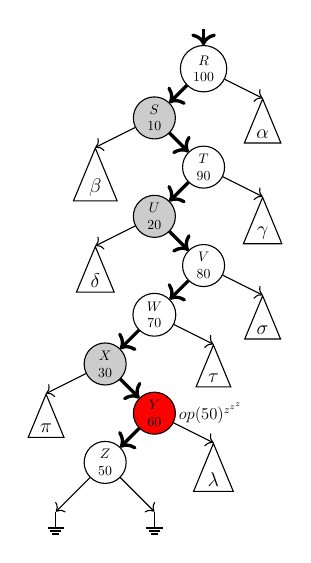
\begin{tikzpicture}[scale=0.5, transform shape] 
	 \newcommand\NODEDX{1.25}
	 \newcommand\NODEDY{1.25}
	 \newcommand\SUBTREEDX{1.5}
	 \newcommand\SUBTREEDY{0.75}
	
   \node (r)	[treenode] 		                at (0, 0)       		                      	{$R$ \\ 100};
   \node (s)	[treenode, fill=black!20] 		at ([shift=({ -\NODEDX, -\NODEDY})]r)     	{$S$ \\ 10};
	 \node (t)	[treenode] 		                at ([shift=({  \NODEDX, -\NODEDY})]s)    		{$T$ \\ 90};
	 \node (u)	[treenode, fill=black!20] 	  at ([shift=({ -\NODEDX, -\NODEDY})]t)     	{$U$ \\ 20};
	 \node (v)	[treenode] 										at ([shift=({  \NODEDX, -\NODEDY})]u)     	{$V$ \\ 80};
	 \node (w)	[treenode] 										at ([shift=({ -\NODEDX, -\NODEDY})]v)     	{$W$ \\ 70};
	 \node (x)	[treenode, fill=black!20] 		at ([shift=({ -\NODEDX, -\NODEDY})]w)     	{$X$ \\ 30};
	 \node (y)	[treenode,fill=red]						at ([shift=({  \NODEDX, -\NODEDY})]x)     	{$Y$ \\ 60};
	 \node (z)	[treenode] 										at ([shift=({ -\NODEDX, -\NODEDY})]y)     	{$Z$ \\ 50};
	 \node (gl) [ground]                      at ([shift=({ -\NODEDX, -\NODEDY})]z)     	{ };
	 \node (gr) [ground]                      at ([shift=({  \NODEDX, -\NODEDY})]z)     	{ };
		
	 \node (sa) [subtree]                     at ([shift=({  \SUBTREEDX, -\SUBTREEDY})]r) {\Large $\alpha$};
	 \node (sb) [subtree]                     at ([shift=({ -\SUBTREEDX, -\SUBTREEDY})]s) {\Large $\beta$};
	 \node (sg) [subtree]                     at ([shift=({  \SUBTREEDX, -\SUBTREEDY})]t) {\Large $\gamma$};
	 \node (sd) [subtree]                     at ([shift=({ -\SUBTREEDX, -\SUBTREEDY})]u) {\Large $\delta$};
	 \node (ss) [subtree]                     at ([shift=({  \SUBTREEDX, -\SUBTREEDY})]v) {\Large $\sigma$};
	 \node (st) [subtree]                     at ([shift=({  \SUBTREEDX, -\SUBTREEDY})]w) {\Large $\tau$};
	 \node (sp) [subtree]                     at ([shift=({ -\SUBTREEDX, -\SUBTREEDY})]x) {\Large $\pi$};
	 \node (sl) [subtree]                     at ([shift=({  \SUBTREEDX, -\SUBTREEDY})]y) {\Large $\lambda$};	
	
	 \node (op) [label={right:{\large $op(50)^{z^{z^z}}$}}] at ([shift=({0.375, 0})]y) {};
	
	 \path[every node/.style={font=\sffamily\small}]
	    (0, 1)  edge[->,very thick]  node {} (r)
		  (r)     edge[->,very thick]  node {} (s)
			(s)     edge[->,very thick]  node {} (t)
			(t)     edge[->,very thick]  node {} (u)
			(u)     edge[->,very thick]  node {} (v)
			(v)     edge[->,very thick]  node {} (w)
			(w)     edge[->,very thick]  node {} (x)
			(x)     edge[->,very thick]  node {} (y)
			(y)     edge[->,very thick]  node {} (z)
			(z)     edge[->]  node {} (gl)
			(z)     edge[->]  node {} (gr)
			(r)     edge[->]  node {} (sa.north)
			(s)     edge[->]  node {} (sb.north)
			(t)     edge[->]  node {} (sg.north)
			(u)     edge[->]  node {} (sd.north)
			(v)     edge[->]  node {} (ss.north)
			(w)     edge[->]  node {} (st.north)
			(x)     edge[->]  node {} (sp.north)
			(y)     edge[->]  node {} (sl.north);		
\end{tikzpicture}
\caption{Operation $op(50)$ is suspended at node $Y$ during its traversal}
\end{figure}
\end{frame}

\begin{frame}[c]{Example}
\begin{figure}[htp]
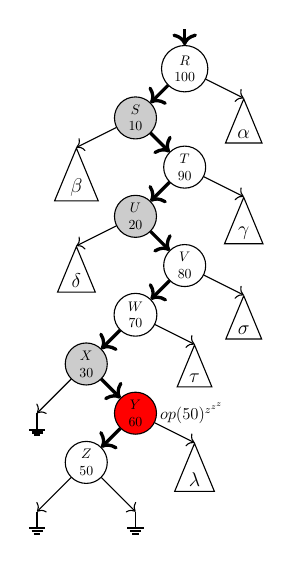
\begin{tikzpicture}[scale=0.5, transform shape]   
	 \newcommand\NODEDX{1.25}
	 \newcommand\NODEDY{1.25}
	 \newcommand\SUBTREEDX{1.5}
	 \newcommand\SUBTREEDY{0.75}
	
   \node (r)	[treenode] 		                at (0, 0)       		                      	{$R$ \\ 100};
   \node (s)	[treenode, fill=black!20] 		at ([shift=({ -\NODEDX, -\NODEDY})]r)     	{$S$ \\ 10};
	 \node (t)	[treenode] 		                at ([shift=({  \NODEDX, -\NODEDY})]s)    		{$T$ \\ 90};
	 \node (u)	[treenode, fill=black!20] 	  at ([shift=({ -\NODEDX, -\NODEDY})]t)     	{$U$ \\ 20};
	 \node (v)	[treenode] 										at ([shift=({  \NODEDX, -\NODEDY})]u)     	{$V$ \\ 80};
	 \node (w)	[treenode] 										at ([shift=({ -\NODEDX, -\NODEDY})]v)     	{$W$ \\ 70};
	 \node (x)	[treenode, fill=black!20] 		at ([shift=({ -\NODEDX, -\NODEDY})]w)     	{$X$ \\ 30};
	 \node (y)	[treenode, fill=red]					at ([shift=({  \NODEDX, -\NODEDY})]x)     	{$Y$ \\ 60};
	 \node (z)	[treenode] 										at ([shift=({ -\NODEDX, -\NODEDY})]y)     	{$Z$ \\ 50};
	 \node (gl) [ground]                      at ([shift=({ -\NODEDX, -\NODEDY})]z)     	{ };
	 \node (gr) [ground]                      at ([shift=({  \NODEDX, -\NODEDY})]z)     	{ };

	 \node (sa) [subtree]                     at ([shift=({  \SUBTREEDX, -\SUBTREEDY})]r) {\Large $\alpha$};
	 \node (sb) [subtree]                     at ([shift=({ -\SUBTREEDX, -\SUBTREEDY})]s) {\Large $\beta$};
	 \node (sg) [subtree]                     at ([shift=({  \SUBTREEDX, -\SUBTREEDY})]t) {\Large $\gamma$};
	 \node (sd) [subtree]                     at ([shift=({ -\SUBTREEDX, -\SUBTREEDY})]u) {\Large $\delta$};
	 \node (ss) [subtree]                     at ([shift=({  \SUBTREEDX, -\SUBTREEDY})]v) {\Large $\sigma$};
	 \node (st) [subtree]                     at ([shift=({  \SUBTREEDX, -\SUBTREEDY})]w) {\Large $\tau$};
	 %% \node (sp) [subtree]                     at ([shift=({ -\SUBTREEDX, -\SUBTREEDY})]x) {\Large $\pi$};
	 \node (sp) [ground]                    	at ([shift=({ -\NODEDX, -\NODEDY})]x) { };
	 \node (sl) [subtree]                     at ([shift=({  \SUBTREEDX, -\SUBTREEDY})]y) {\Large $\lambda$};	

   \node (op) [label={right:{\large $op(50)^{z^{z^z}}$}}] at ([shift=({0.375, 0})]y) {};
	
	 \path[every node/.style={font=\sffamily\small}]
	    (0, 1)  edge[->,very thick]  node {} (r)
		  (r)     edge[->,very thick]  node {} (s)
			(s)     edge[->,very thick]  node {} (t)
			(t)     edge[->,very thick]  node {} (u)
			(u)     edge[->,very thick]  node {} (v)
			(v)     edge[->,very thick]  node {} (w)
			(w)     edge[->,very thick]  node {} (x)
			(x)     edge[->,very thick]  node {} (y)
			(y)     edge[->,very thick]  node {} (z)
			(z)     edge[->]  node {} (gl)
			(z)     edge[->]  node {} (gr)
			(r)     edge[->]  node {} (sa.north)
			(s)     edge[->]  node {} (sb.north)
			(t)     edge[->]  node {} (sg.north)
			(u)     edge[->]  node {} (sd.north)
			(v)     edge[->]  node {} (ss.north)
			(w)     edge[->]  node {} (st.north)
			(x)     edge[->]  node {} (sp)
			(y)     edge[->]  node {} (sl.north);	
\end{tikzpicture}
\caption{All keys in subtree $\pi$ are deleted one-by-one}
\end{figure}
\end{frame}

\begin{frame}[c]{Example}
\begin{figure}[htp]
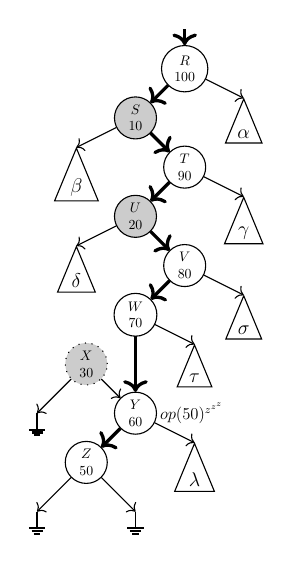
\begin{tikzpicture}[scale=0.5, transform shape]
   
	 \newcommand\NODEDX{1.25}
	 \newcommand\NODEDY{1.25}
	 \newcommand\SUBTREEDX{1.5}
	 \newcommand\SUBTREEDY{0.75}
	
   \node (r)	[treenode] 		                at (0, 0)       		                      	{$R$ \\ 100};
   \node (s)	[treenode, fill=black!20] 		at ([shift=({ -\NODEDX, -\NODEDY})]r)     	{$S$ \\ 10};
	 \node (t)	[treenode] 		                at ([shift=({  \NODEDX, -\NODEDY})]s)    		{$T$ \\ 90};
	 \node (u)	[treenode, fill=black!20] 	  at ([shift=({ -\NODEDX, -\NODEDY})]t)     	{$U$ \\ 20};
	 \node (v)	[treenode] 										at ([shift=({  \NODEDX, -\NODEDY})]u)     	{$V$ \\ 80};
	 \node (w)	[treenode] 										at ([shift=({ -\NODEDX, -\NODEDY})]v)     	{$W$ \\ 70};
	 \node (x)	[treenode, fill=black!20, dotted] 		at ([shift=({ -\NODEDX, -\NODEDY})]w)     	{$X$ \\ 30};
	 \node (y)	[treenode] 										at ([shift=({  \NODEDX, -\NODEDY})]x)     	{$Y$ \\ 60};
	 \node (z)	[treenode] 										at ([shift=({ -\NODEDX, -\NODEDY})]y)     	{$Z$ \\ 50};
	 \node (gl) [ground]                      at ([shift=({ -\NODEDX, -\NODEDY})]z)     	{ };
	 \node (gr) [ground]                      at ([shift=({  \NODEDX, -\NODEDY})]z)     	{ };
		
	 \node (sa) [subtree]                     at ([shift=({  \SUBTREEDX, -\SUBTREEDY})]r) {\Large $\alpha$};
	 \node (sb) [subtree]                     at ([shift=({ -\SUBTREEDX, -\SUBTREEDY})]s) {\Large $\beta$};
	 \node (sg) [subtree]                     at ([shift=({  \SUBTREEDX, -\SUBTREEDY})]t) {\Large $\gamma$};
	 \node (sd) [subtree]                     at ([shift=({ -\SUBTREEDX, -\SUBTREEDY})]u) {\Large $\delta$};
	 \node (ss) [subtree]                     at ([shift=({  \SUBTREEDX, -\SUBTREEDY})]v) {\Large $\sigma$};
	 \node (st) [subtree]                     at ([shift=({  \SUBTREEDX, -\SUBTREEDY})]w) {\Large $\tau$};
	 %% \node (sp) [subtree]                     at ([shift=({ -\SUBTREEDX, -\SUBTREEDY})]x) {\Large $\pi$};
	 \node (sp) [ground]                    	at ([shift=({ -\NODEDX, -\NODEDY})]x) { };
	 \node (sl) [subtree]                     at ([shift=({  \SUBTREEDX, -\SUBTREEDY})]y) {\Large $\lambda$};	
	
	 \node (op) [label={right:{\large $op(50)^{z^{z^z}}$}}] at ([shift=({0.375, 0})]y) {};
	
	 \path[every node/.style={font=\sffamily\small}]
	    (0, 1)  edge[->,very thick]  node {} (r)
		  (r)     edge[->,very thick]  node {} (s)
			(s)     edge[->,very thick]  node {} (t)
			(t)     edge[->,very thick]  node {} (u)
			(u)     edge[->,very thick]  node {} (v)
			(v)     edge[->,very thick]  node {} (w)
			%% (w)     edge[->]  node {} (x)
			(w)     edge[->,very thick]  node {} (y)
			(x)     edge[->]  node {} (y)
			(y)     edge[->,very thick]  node {} (z)
			(z)     edge[->]  node {} (gl)
			(z)     edge[->]  node {} (gr)
			(r)     edge[->]  node {} (sa.north)
			(s)     edge[->]  node {} (sb.north)
			(t)     edge[->]  node {} (sg.north)
			(u)     edge[->]  node {} (sd.north)
			(v)     edge[->]  node {} (ss.north)
			(w)     edge[->]  node {} (st.north)
			(x)     edge[->]  node {} (sp)
			(y)     edge[->]  node {} (sl.north);	
\end{tikzpicture}
\caption{Key 30 is deleted (simple delete); node $X$ is removed}
\end{figure}
\end{frame}

\begin{frame}[c]{Example}
\begin{figure}[htp]
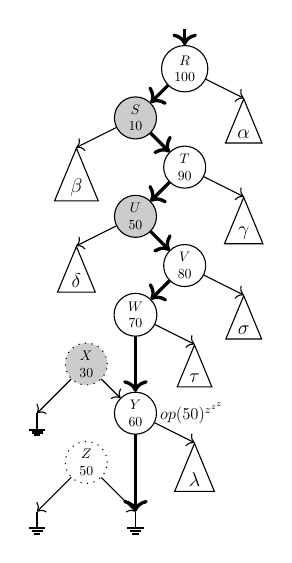
\begin{tikzpicture}[scale=0.5, transform shape]
   
	 \newcommand\NODEDX{1.25}
	 \newcommand\NODEDY{1.25}
	 \newcommand\SUBTREEDX{1.5}
	 \newcommand\SUBTREEDY{0.75}
	
   \node (r)	[treenode] 		                at (0, 0)       		                      	{$R$ \\ 100};
   \node (s)	[treenode, fill=black!20] 		at ([shift=({ -\NODEDX, -\NODEDY})]r)     	{$S$ \\ 10};
	 \node (t)	[treenode] 		                at ([shift=({  \NODEDX, -\NODEDY})]s)    		{$T$ \\ 90};
	 \node (u)	[treenode, fill=black!20] 	  at ([shift=({ -\NODEDX, -\NODEDY})]t)     	{$U$ \\ 50};
	 \node (v)	[treenode] 										at ([shift=({  \NODEDX, -\NODEDY})]u)     	{$V$ \\ 80};
	 \node (w)	[treenode] 										at ([shift=({ -\NODEDX, -\NODEDY})]v)     	{$W$ \\ 70};
	 \node (x)	[treenode, fill=black!20, dotted] 		at ([shift=({ -\NODEDX, -\NODEDY})]w)     	{$X$ \\ 30};
	 \node (y)	[treenode] 										at ([shift=({  \NODEDX, -\NODEDY})]x)     	{$Y$ \\ 60};
	 \node (z)	[treenode, dotted] 						at ([shift=({ -\NODEDX, -\NODEDY})]y)     	{$Z$ \\ 50};
	 \node (gl) [ground]                      at ([shift=({ -\NODEDX, -\NODEDY})]z)     	{ };
	 \node (gr) [ground]                      at ([shift=({  \NODEDX, -\NODEDY})]z)     	{ };
		
	 \node (sa) [subtree]                     at ([shift=({  \SUBTREEDX, -\SUBTREEDY})]r) {\Large $\alpha$};
	 \node (sb) [subtree]                     at ([shift=({ -\SUBTREEDX, -\SUBTREEDY})]s) {\Large $\beta$};
	 \node (sg) [subtree]                     at ([shift=({  \SUBTREEDX, -\SUBTREEDY})]t) {\Large $\gamma$};
	 \node (sd) [subtree]                     at ([shift=({ -\SUBTREEDX, -\SUBTREEDY})]u) {\Large $\delta$};
	 \node (ss) [subtree]                     at ([shift=({  \SUBTREEDX, -\SUBTREEDY})]v) {\Large $\sigma$};
	 \node (st) [subtree]                     at ([shift=({  \SUBTREEDX, -\SUBTREEDY})]w) {\Large $\tau$};
	 %% \node (sp) [subtree]                     at ([shift=({ -\SUBTREEDX, -\SUBTREEDY})]x) {\Large $\pi$};
	 \node (sp) [ground]                    	at ([shift=({ -\NODEDX, -\NODEDY})]x) { };
	 \node (sl) [subtree]                     at ([shift=({  \SUBTREEDX, -\SUBTREEDY})]y) {\Large $\lambda$};	
	
	 \node (op) [label={right:{\large $op(50)^{z^{z^z}}$}}] at ([shift=({0.375, 0})]y) {};
	
	 \path[every node/.style={font=\sffamily\small}]
	    (0, 1)  edge[->,very thick]  node {} (r)
		  (r)     edge[->,very thick]  node {} (s)
			(s)     edge[->,very thick]  node {} (t)
			(t)     edge[->,very thick]  node {} (u)
			(u)     edge[->,very thick]  node {} (v)
			(v)     edge[->,very thick]  node {} (w)
			%% (w)     edge[->]  node {} (x)
			(w)     edge[->,very thick]  node {} (y)
			(x)     edge[->]  node {} (y)
			%% (y)     edge[->]  node {} (z)
			(y)     edge[->, very thick]  node {} (gr)
			(z)     edge[->]  node {} (gl)
			(z)     edge[->]  node {} (gr)
			(r)     edge[->]  node {} (sa.north)
			(s)     edge[->]  node {} (sb.north)
			(t)     edge[->]  node {} (sg.north)
			(u)     edge[->]  node {} (sd.north)
			(v)     edge[->]  node {} (ss.north)
			(w)     edge[->]  node {} (st.north)
			(x)     edge[->]  node {} (sp)
			(y)     edge[->]  node {} (sl.north);		
\end{tikzpicture}
\caption{Key 20 is deleted (complex delete); key 20 is replaced with key 50 in node $U$ and node $Z$ is removed}
\end{figure}
\end{frame}

\begin{frame}[c]{Traversal Stack}
\begin{itemize}
\item a stack to keep track of anchor nodes of all nodes in the traversal path
\item reduces tree traversal cost during failures by restarting closer to an operation�s window
\end{itemize}
\end{frame}

\begin{frame}[c]{Traversal Stack}
\begin{figure}[htp]
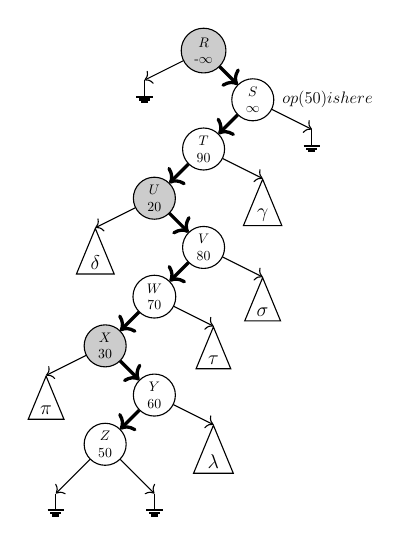
\begin{tikzpicture}[scale=0.5, transform shape] 
	 \newcommand\NODEDX{1.25}
	 \newcommand\NODEDY{1.25}
	 \newcommand\SUBTREEDX{1.5}
	 \newcommand\SUBTREEDY{0.75}
	
   \node (r)	[treenode, fill=black!20] 		at (0, 0)       		                      	{$R$ \\  -$\infty$};
   \node (s)	[treenode] 										at ([shift=({ \NODEDX, -\NODEDY})]r)     	  {$S$ \\  $\infty$};
	 \node (t)	[treenode] 		                at ([shift=({  -\NODEDX, -\NODEDY})]s)    	{$T$ \\ 90};
	 \node (u)	[treenode, fill=black!20] 	  at ([shift=({ -\NODEDX, -\NODEDY})]t)     	{$U$ \\ 20};
	 \node (v)	[treenode] 										at ([shift=({  \NODEDX, -\NODEDY})]u)     	{$V$ \\ 80};
	 \node (w)	[treenode] 										at ([shift=({ -\NODEDX, -\NODEDY})]v)     	{$W$ \\ 70};
	 \node (x)	[treenode, fill=black!20] 		at ([shift=({ -\NODEDX, -\NODEDY})]w)     	{$X$ \\ 30};
	 \node (y)	[treenode] 										at ([shift=({  \NODEDX, -\NODEDY})]x)     	{$Y$ \\ 60};
	 \node (z)	[treenode] 										at ([shift=({ -\NODEDX, -\NODEDY})]y)     	{$Z$ \\ 50};
	 \node (gl) [ground]                      at ([shift=({ -\NODEDX, -\NODEDY})]z)     	{ };
	 \node (gr) [ground]                      at ([shift=({  \NODEDX, -\NODEDY})]z)     	{ };
		
	 \node (sa) [ground]                      at ([shift=({ -\SUBTREEDX, -\SUBTREEDY})]r) { };
	 \node (sb) [ground]                      at ([shift=({ \SUBTREEDX, -\SUBTREEDY})]s) 	{ };
	 \node (sg) [subtree]                     at ([shift=({  \SUBTREEDX, -\SUBTREEDY})]t) {\Large $\gamma$};
	 \node (sd) [subtree]                     at ([shift=({ -\SUBTREEDX, -\SUBTREEDY})]u) {\Large $\delta$};
	 \node (ss) [subtree]                     at ([shift=({  \SUBTREEDX, -\SUBTREEDY})]v) {\Large $\sigma$};
	 \node (st) [subtree]                     at ([shift=({  \SUBTREEDX, -\SUBTREEDY})]w) {\Large $\tau$};
	 \node (sp) [subtree]                     at ([shift=({ -\SUBTREEDX, -\SUBTREEDY})]x) {\Large $\pi$};
	 \node (sl) [subtree]                     at ([shift=({  \SUBTREEDX, -\SUBTREEDY})]y) {\Large $\lambda$};	
	
	 \node (op) [label={right:{\large $op(50) is here$}}] at ([shift=({0.5, 0})]s) {};
	
	 \path[every node/.style={font=\sffamily\small}]
	    %(0, 1)  edge[->,very thick]  node {} (r)
		  (r)     edge[->,very thick]  node {} (s)
			(s)     edge[->,very thick]  node {} (t)
			(t)     edge[->,very thick]  node {} (u)
			(u)     edge[->,very thick]  node {} (v)
			(v)     edge[->,very thick]  node {} (w)
			(w)     edge[->,very thick]  node {} (x)
			(x)     edge[->,very thick]  node {} (y)
			(y)     edge[->,very thick]  node {} (z)
			(z)     edge[->]  node {} (gl)
			(z)     edge[->]  node {} (gr)
			(r)     edge[->]  node {} (sa)
			(s)     edge[->]  node {} (sb)
			(t)     edge[->]  node {} (sg.north)
			(u)     edge[->]  node {} (sd.north)
			(v)     edge[->]  node {} (ss.north)
			(w)     edge[->]  node {} (st.north)
			(x)     edge[->]  node {} (sp.north)
			(y)     edge[->]  node {} (sl.north);		
\end{tikzpicture}
%\qquad
%\begin{tikzpicture}[scale=1.0, transform shape]
%\node[stack=9]  {
%0,\nodepart{one}Z,left,6
%\nodepart{two}Y,rigt,6
%\nodepart{three}X,left,3
%\nodepart{four}W,left,3
%\nodepart{five}V,right,3
%\nodepart{six}U,left,1
%\nodepart{seven}T,right,1
%\nodepart{eight}S,right,0
%\nodepart{nine}R,right,-1
%};
%\end{tikzpicture}
\qquad
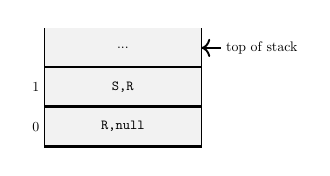
\begin{tikzpicture}[scale=0.5, transform shape]
  \stacktop{} \cellptr{top of stack}
	\separator
	\cell{\texttt{S,R}}        \cellcomL{1} \coordinate () at (currentcell.east);
  \separator
	\cell{\texttt{R,null}}     \cellcomL{0} \coordinate () at (currentcell.east);
  \separator
\end{tikzpicture}
\caption{Operation $op(50)$ starting at R and ending at Z along with the stack}
\end{figure}
\end{frame}
\begin{frame}[c]{Traversal Stack}
\begin{figure}[htp]
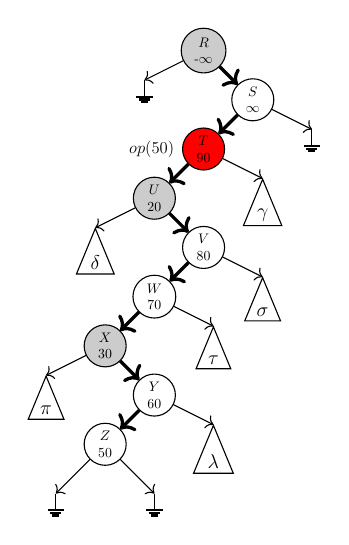
\begin{tikzpicture}[scale=0.5, transform shape] 
	 \newcommand\NODEDX{1.25}
	 \newcommand\NODEDY{1.25}
	 \newcommand\SUBTREEDX{1.5}
	 \newcommand\SUBTREEDY{0.75}
	
   \node (r)	[treenode, fill=black!20] 		at (0, 0)       		                      	{$R$ \\  -$\infty$};
   \node (s)	[treenode] 										at ([shift=({ \NODEDX, -\NODEDY})]r)     	  {$S$ \\  $\infty$};
	 \node (t)	[treenode, fill=red]          at ([shift=({  -\NODEDX, -\NODEDY})]s)    	{$T$ \\ 90};
	 \node (u)	[treenode, fill=black!20] 	  at ([shift=({ -\NODEDX, -\NODEDY})]t)     	{$U$ \\ 20};
	 \node (v)	[treenode] 										at ([shift=({  \NODEDX, -\NODEDY})]u)     	{$V$ \\ 80};
	 \node (w)	[treenode] 										at ([shift=({ -\NODEDX, -\NODEDY})]v)     	{$W$ \\ 70};
	 \node (x)	[treenode, fill=black!20] 		at ([shift=({ -\NODEDX, -\NODEDY})]w)     	{$X$ \\ 30};
	 \node (y)	[treenode] 										at ([shift=({  \NODEDX, -\NODEDY})]x)     	{$Y$ \\ 60};
	 \node (z)	[treenode] 										at ([shift=({ -\NODEDX, -\NODEDY})]y)     	{$Z$ \\ 50};
	 \node (gl) [ground]                      at ([shift=({ -\NODEDX, -\NODEDY})]z)     	{ };
	 \node (gr) [ground]                      at ([shift=({  \NODEDX, -\NODEDY})]z)     	{ };
		
	 \node (sa) [ground]                      at ([shift=({ -\SUBTREEDX, -\SUBTREEDY})]r) { };
	 \node (sb) [ground]                      at ([shift=({ \SUBTREEDX, -\SUBTREEDY})]s) 	{ };
	 \node (sg) [subtree]                     at ([shift=({  \SUBTREEDX, -\SUBTREEDY})]t) {\Large $\gamma$};
	 \node (sd) [subtree]                     at ([shift=({ -\SUBTREEDX, -\SUBTREEDY})]u) {\Large $\delta$};
	 \node (ss) [subtree]                     at ([shift=({  \SUBTREEDX, -\SUBTREEDY})]v) {\Large $\sigma$};
	 \node (st) [subtree]                     at ([shift=({  \SUBTREEDX, -\SUBTREEDY})]w) {\Large $\tau$};
	 \node (sp) [subtree]                     at ([shift=({ -\SUBTREEDX, -\SUBTREEDY})]x) {\Large $\pi$};
	 \node (sl) [subtree]                     at ([shift=({  \SUBTREEDX, -\SUBTREEDY})]y) {\Large $\lambda$};	
	
	 \node (op) [label={left:{\large $op(50)$}}] at ([shift=({-0.5, 0})]t) {};
	
	 \path[every node/.style={font=\sffamily\small}]
	    %(0, 1)  edge[->,very thick]  node {} (r)
		  (r)     edge[->,very thick]  node {} (s)
			(s)     edge[->,very thick]  node {} (t)
			(t)     edge[->,very thick]  node {} (u)
			(u)     edge[->,very thick]  node {} (v)
			(v)     edge[->,very thick]  node {} (w)
			(w)     edge[->,very thick]  node {} (x)
			(x)     edge[->,very thick]  node {} (y)
			(y)     edge[->,very thick]  node {} (z)
			(z)     edge[->]  node {} (gl)
			(z)     edge[->]  node {} (gr)
			(r)     edge[->]  node {} (sa)
			(s)     edge[->]  node {} (sb)
			(t)     edge[->]  node {} (sg.north)
			(u)     edge[->]  node {} (sd.north)
			(v)     edge[->]  node {} (ss.north)
			(w)     edge[->]  node {} (st.north)
			(x)     edge[->]  node {} (sp.north)
			(y)     edge[->]  node {} (sl.north);		
\end{tikzpicture}
%\qquad
%\begin{tikzpicture}[scale=1.0, transform shape]
%\node[stack=9]  {
%0,\nodepart{one}Z,left,6
%\nodepart{two}Y,rigt,6
%\nodepart{three}X,left,3
%\nodepart{four}W,left,3
%\nodepart{five}V,right,3
%\nodepart{six}U,left,1
%\nodepart{seven}T,right,1
%\nodepart{eight}S,right,0
%\nodepart{nine}R,right,-1
%};
%\end{tikzpicture}
\qquad
\begin{tikzpicture}[scale=0.5, transform shape]
  \stacktop{} \cellptr{top of stack}
	\separator
	\cell{\Large \texttt{T,R}}        \cellcomL{2} \coordinate () at (currentcell.east);
  \separator
	\cell{\Large \texttt{S,R}}        \cellcomL{1} \coordinate () at (currentcell.east);
  \separator
	\cell{\Large \texttt{R,null}}     \cellcomL{0} \coordinate () at (currentcell.east);
  \separator
\end{tikzpicture}
%\caption{Operation $op(50)$ starting at R and suspended at Y along with the stack}
\end{figure}
\end{frame}


\begin{frame}[c]{Search}
search operations do not restart
\begin{figure}[htp]
\centering
{
	\begin{tikzpicture}[scale=0.5, transform shape]
	\node (p0) [] {search(K)};
	\node (p1) [process, below of=p0, text width=4cm] {Do a binary search for key K in the tree};
	\node (p2) [process, below of=p1, yshift=-1.5cm, text width=4.5cm] {Examine anchor node $A$ of top entry in the stack};
	\node (p3) [decision, below of=p2, yshift=-1.5cm, text width=2cm] {is anchor node marked?};
	\node (p4) [process, right of=p3, xshift=4cm, text width=4.5cm] {pop all entries upto anchor node $A$};
	\node (retT) [process, right of=p1, xshift=4cm, text width=1cm, minimum width=1cm] {return true};
	\node (retF) [process, left of=p2, xshift=-5cm, text width=1cm, minimum width=1cm] {return false};

	\draw [arrow] (p1) -- node[anchor=west] {K not found} (p2);
	\draw [arrow] (p1) -- node[anchor=south] {K found} (retT);
	\draw [arrow] (p2.east) -| node[anchor=north,pos=0.5] {K = A.key}    (retT.south);
	\draw [arrow] (p2.west) -- node (temp) [anchor=north,pos=0.5] {K $<$ A.key}  (retF.east);
	\draw [arrow] (p2) -- node[anchor=east] {K $>$ A.key} (p3);
	\draw [arrow] (p3.west) -| (retF.south) node[below, pos=0.5]{No}  (retF.south);
	\draw [arrow] (p3.east) -- node[anchor=north]{Yes} (p4.west);
	\draw [arrow] (p4.north) -- (p2.south);
	\node (temp1) [above of=temp,xshift=0.5cm,yshift=0.4cm] {(Aold.key $<$ K $<$ Anew.key)};
	\end{tikzpicture}
}
\caption{Sequence of steps in a search operation}
\end{figure}
\end{frame}

\begin{frame}[c]{Search}
\begin{figure}[htp]
\begin{tikzpicture}[scale=0.5, transform shape] 
	 \newcommand\NODEDX{1.25}
	 \newcommand\NODEDY{1.25}
	 \newcommand\SUBTREEDX{1.5}
	 \newcommand\SUBTREEDY{0.75}
	
   \node (r)	[treenode, fill=black!20] 		at (0, 0)       		                      	{$R$ \\  -$\infty$};
   \node (s)	[treenode] 										at ([shift=({ \NODEDX, -\NODEDY})]r)     	  {$S$ \\  $\infty$};
	 \node (t)	[treenode, fill=red]          at ([shift=({  -\NODEDX, -\NODEDY})]s)    	{$T$ \\ 90};
	 \node (u)	[treenode, fill=black!20] 	  at ([shift=({ -\NODEDX, -\NODEDY})]t)     	{$U$ \\ 20};
	 \node (v)	[treenode] 										at ([shift=({  \NODEDX, -\NODEDY})]u)     	{$V$ \\ 80};
	 \node (w)	[treenode] 										at ([shift=({ -\NODEDX, -\NODEDY})]v)     	{$W$ \\ 70};
	 \node (x)	[treenode, fill=black!20] 		at ([shift=({ -\NODEDX, -\NODEDY})]w)     	{$X$ \\ 30};
	 \node (y)	[treenode] 										at ([shift=({  \NODEDX, -\NODEDY})]x)     	{$Y$ \\ 60};
	 \node (z)	[treenode] 										at ([shift=({ -\NODEDX, -\NODEDY})]y)     	{$Z$ \\ 50};
	 \node (gl) [ground]                      at ([shift=({ -\NODEDX, -\NODEDY})]z)     	{ };
	 \node (gr) [ground]                      at ([shift=({  \NODEDX, -\NODEDY})]z)     	{ };
		
	 \node (sa) [ground]                      at ([shift=({ -\SUBTREEDX, -\SUBTREEDY})]r) { };
	 \node (sb) [ground]                      at ([shift=({ \SUBTREEDX, -\SUBTREEDY})]s) 	{ };
	 \node (sg) [subtree]                     at ([shift=({  \SUBTREEDX, -\SUBTREEDY})]t) {\Large $\gamma$};
	 \node (sd) [subtree]                     at ([shift=({ -\SUBTREEDX, -\SUBTREEDY})]u) {\Large $\delta$};
	 \node (ss) [subtree]                     at ([shift=({  \SUBTREEDX, -\SUBTREEDY})]v) {\Large $\sigma$};
	 \node (st) [subtree]                     at ([shift=({  \SUBTREEDX, -\SUBTREEDY})]w) {\Large $\tau$};
	 \node (sp) [subtree]                     at ([shift=({ -\SUBTREEDX, -\SUBTREEDY})]x) {\Large $\pi$};
	 \node (sl) [subtree]                     at ([shift=({  \SUBTREEDX, -\SUBTREEDY})]y) {\Large $\lambda$};	
	
	 \node (op) [label={left:{\large $op(50)$}}] at ([shift=({-0.5, 0})]t) {};
	
	 \path[every node/.style={font=\sffamily\small}]
	    %(0, 1)  edge[->,very thick]  node {} (r)
		  (r)     edge[->,very thick]  node {} (s)
			(s)     edge[->,very thick]  node {} (t)
			(t)     edge[->,very thick]  node {} (u)
			(u)     edge[->,very thick]  node {} (v)
			(v)     edge[->,very thick]  node {} (w)
			(w)     edge[->,very thick]  node {} (x)
			(x)     edge[->,very thick]  node {} (y)
			(y)     edge[->,very thick]  node {} (z)
			(z)     edge[->]  node {} (gl)
			(z)     edge[->]  node {} (gr)
			(r)     edge[->]  node {} (sa)
			(s)     edge[->]  node {} (sb)
			(t)     edge[->]  node {} (sg.north)
			(u)     edge[->]  node {} (sd.north)
			(v)     edge[->]  node {} (ss.north)
			(w)     edge[->]  node {} (st.north)
			(x)     edge[->]  node {} (sp.north)
			(y)     edge[->]  node {} (sl.north);		
\end{tikzpicture}
%\qquad
%\begin{tikzpicture}[scale=1.0, transform shape]
%\node[stack=9]  {
%0,\nodepart{one}Z,left,6
%\nodepart{two}Y,rigt,6
%\nodepart{three}X,left,3
%\nodepart{four}W,left,3
%\nodepart{five}V,right,3
%\nodepart{six}U,left,1
%\nodepart{seven}T,right,1
%\nodepart{eight}S,right,0
%\nodepart{nine}R,right,-1
%};
%\end{tikzpicture}
\qquad
\begin{tikzpicture}[scale=0.5, transform shape]
  \stacktop{} \cellptr{top of stack}
	\separator
	\cell{\Large \texttt{T,R}}        \cellcomL{2} \coordinate () at (currentcell.east);
  \separator
	\cell{\Large \texttt{S,R}}        \cellcomL{1} \coordinate () at (currentcell.east);
  \separator
	\cell{\Large \texttt{R,null}}     \cellcomL{0} \coordinate () at (currentcell.east);
  \separator
\end{tikzpicture}
%\caption{Operation $op(50)$ starting at R and suspended at Y along with the stack}
\end{figure}
\end{frame}
\begin{frame}[c]{Search}
\begin{figure}[htp]
\begin{tikzpicture}[scale=0.33, transform shape]
   
	 \newcommand\NODEDX{1.25}
	 \newcommand\NODEDY{1.25}
	 \newcommand\SUBTREEDX{1.5}
	 \newcommand\SUBTREEDY{0.75}
	
	 \node (r)	[treenode, fill=black!20] 		at (0, 0)       		                      	{$R$ \\  -$\infty$};
   \node (s)	[treenode] 										at ([shift=({ \NODEDX, -\NODEDY})]r)     	  {$S$ \\  $\infty$};
	 \node (t)	[treenode] 		                at ([shift=({  -\NODEDX, -\NODEDY})]s)    	{$T$ \\ 90};
	 \node (u)	[treenode, fill=black!20] 	  at ([shift=({ -\NODEDX, -\NODEDY})]t)     	{$U$ \\ 50};
	 \node (v)	[treenode] 										at ([shift=({  \NODEDX, -\NODEDY})]u)     	{$V$ \\ 80};
	 \node (w)	[treenode] 										at ([shift=({ -\NODEDX, -\NODEDY})]v)     	{$W$ \\ 70};
	 \node (x)	[treenode, fill=black!20, dotted] 		at ([shift=({ -\NODEDX, -\NODEDY})]w)     	{$X$ \\ 30};
	 \node (y)	[treenode] 										at ([shift=({  \NODEDX, -\NODEDY})]x)     	{$Y$ \\ 60};
	 \node (z)	[treenode, dotted] 						at ([shift=({ -\NODEDX, -\NODEDY})]y)     	{$Z$ \\ 50};
	 \node (gl) [ground]                      at ([shift=({ -\NODEDX, -\NODEDY})]z)     	{ };
	 \node (gr) [ground]                      at ([shift=({  \NODEDX, -\NODEDY})]z)     	{ };
		
	 \node (sa) [ground]                      at ([shift=({ -\SUBTREEDX, -\SUBTREEDY})]r) { };
	 \node (sb) [ground]                      at ([shift=({ \SUBTREEDX, -\SUBTREEDY})]s) 	{ };
	 \node (sg) [subtree]                     at ([shift=({  \SUBTREEDX, -\SUBTREEDY})]t) {\Large $\gamma$};
	 \node (sd) [subtree]                     at ([shift=({ -\SUBTREEDX, -\SUBTREEDY})]u) {\Large $\delta$};
	 \node (ss) [subtree]                     at ([shift=({  \SUBTREEDX, -\SUBTREEDY})]v) {\Large $\sigma$};
	 \node (st) [subtree]                     at ([shift=({  \SUBTREEDX, -\SUBTREEDY})]w) {\Large $\tau$};
	 %% \node (sp) [subtree]                     at ([shift=({ -\SUBTREEDX, -\SUBTREEDY})]x) {\Large $\pi$};
	 \node (sp) [ground]                    	at ([shift=({ -\NODEDX, -\NODEDY})]x) { };
	 \node (sl) [subtree]                     at ([shift=({  \SUBTREEDX, -\SUBTREEDY})]y) {\Large $\lambda$};	
	
	 \node (op) [label={right:{\large $search(50)$}}] at ([shift=({0.375, 0})]gr) {};
	
	 \path[every node/.style={font=\sffamily\small}]
	    %(0, 1)  edge[->,very thick]  node {} (r)
		  (r)     edge[->,very thick]  node {} (s)
			(s)     edge[->,very thick]  node {} (t)
			(t)     edge[->,very thick]  node {} (u)
			(u)     edge[->,very thick]  node {} (v)
			(v)     edge[->,very thick]  node {} (w)
			%% (w)     edge[->]  node {} (x)
			(w)     edge[->,very thick]  node {} (y)
			(x)     edge[->]  node {} (y)
			%% (y)     edge[->]  node {} (z)
			(y)     edge[->, very thick]  node {} (gr)
			(z)     edge[->]  node {} (gl)
			(z)     edge[->]  node {} (gr)
			(r)     edge[->]  node {} (sa)
			(s)     edge[->]  node {} (sb)
			(t)     edge[->]  node {} (sg.north)
			(u)     edge[->]  node {} (sd.north)
			(v)     edge[->]  node {} (ss.north)
			(w)     edge[->]  node {} (st.north)
			(x)     edge[->]  node {} (sp)
			(y)     edge[->]  node {} (sl.north);		
\end{tikzpicture}
\quad
\begin{tikzpicture}[scale=0.28, transform shape]
  \stacktop{} \cellptr{top}
	\separator
	\cell{\Large \texttt{Y,X}}        \cellcomL{7} \coordinate () at (currentcell.east);
  \separator
	\cell{\Large \texttt{X,U}}        \cellcomL{6} \coordinate () at (currentcell.east);
  \separator
	\cell{\Large \texttt{W,U}}        \cellcomL{5} \coordinate () at (currentcell.east);
  \separator
	\cell{\Large \texttt{V,U}}        \cellcomL{4} \coordinate () at (currentcell.east);
  \separator
	\cell{\Large \texttt{U,R}}        \cellcomL{3} \coordinate () at (currentcell.east);
  \separator
	\cell{\Large \texttt{T,R}}        \cellcomL{2} \coordinate () at (currentcell.east);
  \separator
	\cell{\Large \texttt{S,R}}        \cellcomL{1} \coordinate () at (currentcell.east);
  \separator
	\cell{\Large \texttt{R,null}}     \cellcomL{0} \coordinate () at (currentcell.east);
  \separator
\end{tikzpicture}
\quad
\begin{tikzpicture}[scale=0.4, transform shape]
	\node (p0) [] {search(K)};
	\node (p1) [process, below of=p0, text width=4cm] {Do a binary search for key K in the tree};
	\node (p2) [process, below of=p1, yshift=-1.5cm, text width=4.5cm,fill=black!20] {Examine anchor node $A$ of top entry in the stack};
	\node (p3) [decision, below of=p2, yshift=-1.5cm, text width=2cm,fill=black!20] {is anchor node marked?};
	\node (p4) [process, right of=p3, xshift=4cm, text width=4.5cm,fill=black!20] {pop all entries upto anchor node $A$};
	\node (retT) [process, right of=p1, xshift=4cm, text width=1cm, minimum width=1cm] {return true};
	\node (retF) [process, left of=p2, xshift=-5cm, text width=1cm, minimum width=1cm] {return false};

	\draw [arrow] (p1) -- node[anchor=west] {K not found} (p2);
	\draw [arrow] (p1) -- node[anchor=south] {K found} (retT);
	\draw [arrow] (p2.east) -| node[anchor=north,pos=0.5] {K = A.key}    (retT.south);
	\draw [arrow] (p2.west) -- node (temp) [anchor=north,pos=0.5] {K $<$ A.key}  (retF.east);
	\draw [arrow] (p2) -- node[anchor=east] {K $>$ A.key} (p3);
	\draw [arrow] (p3.west) -| (retF.south) node[below, pos=0.5]{No}  (retF.south);
	\draw [arrow] (p3.east) -- node[anchor=north]{Yes} (p4.west);
	\draw [arrow] (p4.north) -- (p2.south);
	\node (temp1) [above of=temp,xshift=0.5cm,yshift=0.4cm] {(A.oldKey $<$ K $<$ A.newKey)};
	\end{tikzpicture}
\caption{Key 30 is deleted;key 20 is deleted $\&$ replaced with key 50 in node $U$ and node $Z$ is removed}
\end{figure}
\end{frame}
\begin{frame}[c]{Search}
\begin{figure}[htp]
\begin{tikzpicture}[scale=0.5, transform shape]
   
	 \newcommand\NODEDX{1.25}
	 \newcommand\NODEDY{1.25}
	 \newcommand\SUBTREEDX{1.5}
	 \newcommand\SUBTREEDY{0.75}
	
	 \node (r)	[treenode, fill=black!20] 		at (0, 0)       		                      	{$R$ \\  -$\infty$};
   \node (s)	[treenode] 										at ([shift=({ \NODEDX, -\NODEDY})]r)     	  {$S$ \\  $\infty$};
	 \node (t)	[treenode] 		                at ([shift=({  -\NODEDX, -\NODEDY})]s)    	{$T$ \\ 90};
	 \node (u)	[treenode, fill=black!20] 	  at ([shift=({ -\NODEDX, -\NODEDY})]t)     	{$U$ \\ 50};
	 \node (v)	[treenode] 										at ([shift=({  \NODEDX, -\NODEDY})]u)     	{$V$ \\ 80};
	 \node (w)	[treenode] 										at ([shift=({ -\NODEDX, -\NODEDY})]v)     	{$W$ \\ 70};
	 \node (x)	[treenode, fill=black!20, dotted] 		at ([shift=({ -\NODEDX, -\NODEDY})]w)     	{$X$ \\ 30};
	 \node (y)	[treenode] 										at ([shift=({  \NODEDX, -\NODEDY})]x)     	{$Y$ \\ 60};
	 \node (z)	[treenode, dotted] 						at ([shift=({ -\NODEDX, -\NODEDY})]y)     	{$Z$ \\ 50};
	 \node (gl) [ground]                      at ([shift=({ -\NODEDX, -\NODEDY})]z)     	{ };
	 \node (gr) [ground]                      at ([shift=({  \NODEDX, -\NODEDY})]z)     	{ };
		
	 \node (sa) [ground]                      at ([shift=({ -\SUBTREEDX, -\SUBTREEDY})]r) { };
	 \node (sb) [ground]                      at ([shift=({ \SUBTREEDX, -\SUBTREEDY})]s) 	{ };
	 \node (sg) [subtree]                     at ([shift=({  \SUBTREEDX, -\SUBTREEDY})]t) {\Large $\gamma$};
	 \node (sd) [subtree]                     at ([shift=({ -\SUBTREEDX, -\SUBTREEDY})]u) {\Large $\delta$};
	 \node (ss) [subtree]                     at ([shift=({  \SUBTREEDX, -\SUBTREEDY})]v) {\Large $\sigma$};
	 \node (st) [subtree]                     at ([shift=({  \SUBTREEDX, -\SUBTREEDY})]w) {\Large $\tau$};
	 %% \node (sp) [subtree]                     at ([shift=({ -\SUBTREEDX, -\SUBTREEDY})]x) {\Large $\pi$};
	 \node (sp) [ground]                    	at ([shift=({ -\NODEDX, -\NODEDY})]x) { };
	 \node (sl) [subtree]                     at ([shift=({  \SUBTREEDX, -\SUBTREEDY})]y) {\Large $\lambda$};	
	
	 \node (op) [label={left:{\large $op(50) is here$}}] at ([shift=({-0.5, 0})]w) {};
	
	 \path[every node/.style={font=\sffamily\small}]
	    %(0, 1)  edge[->,very thick]  node {} (r)
		  (r)     edge[->,very thick]  node {} (s)
			(s)     edge[->,very thick]  node {} (t)
			(t)     edge[->,very thick]  node {} (u)
			(u)     edge[->,very thick]  node {} (v)
			(v)     edge[->,very thick]  node {} (w)
			%% (w)     edge[->]  node {} (x)
			(w)     edge[->,very thick]  node {} (y)
			(x)     edge[->]  node {} (y)
			%% (y)     edge[->]  node {} (z)
			(y)     edge[->, very thick]  node {} (gr)
			(z)     edge[->]  node {} (gl)
			(z)     edge[->]  node {} (gr)
			(r)     edge[->]  node {} (sa)
			(s)     edge[->]  node {} (sb)
			(t)     edge[->]  node {} (sg.north)
			(u)     edge[->]  node {} (sd.north)
			(v)     edge[->]  node {} (ss.north)
			(w)     edge[->]  node {} (st.north)
			(x)     edge[->]  node {} (sp)
			(y)     edge[->]  node {} (sl.north);		
\end{tikzpicture}
\qquad
\begin{tikzpicture}[scale=0.5, transform shape]
  \stacktop{} \cellptr{top of stack}
	\separator
	\cell{\texttt{W,U}}        \cellcomL{5} \coordinate () at (currentcell.east);
  \separator
	\cell{\texttt{V,U}}        \cellcomL{4} \coordinate () at (currentcell.east);
  \separator
	\cell{\texttt{U,R}}        \cellcomL{3} \coordinate () at (currentcell.east);
  \separator
	\cell{\texttt{T,R}}        \cellcomL{2} \coordinate () at (currentcell.east);
  \separator
	\cell{\texttt{S,R}}        \cellcomL{1} \coordinate () at (currentcell.east);
  \separator
	\cell{\texttt{R,null}}     \cellcomL{0} \coordinate () at (currentcell.east);
  \separator
\end{tikzpicture}
\caption{Pop upto marked anchor node $X$. Top of stack is now $W$. Examine anchor node $U$}
\end{figure}
\end{frame}

\begin{frame}[c]{Insert}
An insert operation needs to restart only if one of the anchor nodes in the path has become inconsistent
\begin{figure}[htp]
\centering
{
	\begin{tikzpicture}[scale=0.5, transform shape]
	\node (p0) [] {insert(K)};
	\node (p1) [process, below of=p0, text width=4cm] {Do a binary search for key K in the tree};
	\node (p2) [process, below of=p1, yshift=-1.5cm, text width=4.5cm] {Examine anchor node $A$ of top entry in the stack};
	\node (p3) [decision, below of=p2, yshift=-1.5cm, text width=2cm] {is anchor node marked?};
	\node (p4) [process, right of=p3, xshift=4cm, text width=4.5cm] {pop all entries upto anchor node $A$};
	\node (retF) [process, right of=p1, xshift=4cm, text width=1cm, minimum width=1cm] {return false};
	\node (retT) [process, left of=p2, xshift=-6cm, text width=4.5cm, minimum width=1cm] {discard suffix of the path after anchor node and find a restart point};
	\node (p5) [process, left of=p3, xshift=-6cm, text width=4.5cm, minimum width=1cm] {traversal terminates. Terminal node is returned as the injection point};

	\draw [arrow] (p1) -- node[anchor=west] {K not found} (p2);
	\draw [arrow] (p1) -- node[anchor=south] {K found} (retF);
	\draw [arrow] (p2.east) -| node[anchor=north,pos=0.5] {K = A.key}    (retF.south);
	\draw [arrow] (p2.west) -- node[anchor=north,pos=0.5] {K $<$ A.key}  (retT.east);
	\draw [arrow] (p2) -- node[anchor=east] {K $>$ A.key} (p3);
	\draw [arrow] (p3.west)  -- node[anchor=north]{No}  (p5.east);
	\draw [arrow] (p3.east) -- node[anchor=north]{Yes} (p4.west);
	\draw [arrow] (p4.north) -- (p2.south);

	\end{tikzpicture}
}
\caption{Sequence of steps in an insert operation}
\end{figure}
\end{frame}

\begin{frame}[c]{Delete}
A delete operation do not restart except when there is a failure in the execution phase
\begin{figure}[htp]
\centering
{
	\begin{tikzpicture}[scale=0.5, transform shape]
	\node (p0) [] {delete(K)};
	\node (p1) [process, below of=p0, text width=4cm] {Do a binary search for key K in the tree};
	\node (p2) [process, below of=p1, yshift=-1.5cm, text width=4.5cm] {Examine anchor node $A$ of top entry in the stack};
	\node (p3) [decision, below of=p2, yshift=-1.5cm, text width=2cm] {is anchor node marked?};
	\node (p4) [process, right of=p3, xshift=4cm, text width=4.5cm] {pop all entries upto anchor node $A$};
	\node (ex) [process, right of=p1, xshift=6cm, text width=4.5cm, minimum width=1cm] {go to execution phase};
	\node (retF) [process, left of=p2, xshift=-4cm, text width=1cm, minimum width=1cm] {return false};

	\draw [arrow] (p1) -- node[anchor=west] {K not found} (p2);
	\draw [arrow] (p1) -- node[anchor=south] {K found} (ex);
	\draw [arrow] (p2.east) -| node[anchor=north,pos=0.5] {K = A.key}    (ex.south);
	\draw [arrow] (p2.west) -- node[anchor=north,pos=0.5] {K $<$ A.key}  (retF.east);
	\draw [arrow] (p2) -- node[anchor=east] {K $>$ A.key} (p3);
	\draw [arrow] (p3.west)  -| node[anchor=north]{No}  (retF.south);
	\draw [arrow] (p3.east) -- node[anchor=north]{Yes} (p4.west);
	\draw [arrow] (p4.north) -- (p2.south);

	\end{tikzpicture}
}
\caption{Sequence of steps in a delete operation}
\end{figure}
\end{frame}
%\section{Performance on accelerators}
%\label{sec:experiments:micVsSnb}
%\input{c06/micVsSnb}

\section{Future Work}
\begin{frame}{Future Work}
\begin{itemize}
\item analyze our local recovery algorithm (amortized time complexity)
\item develop concurrent K-ary BST which can improve spatial locality
\item work on other data structures like tries, bloom filters, etc.
\item evaluate using real workloads.
\end{itemize}
\end{frame}

\ifdefined\LONG
\begin{frame}{Future Work - K-ary BST}
\begin{itemize}
\item ideas from Lock Based BST can be extended to external K-ary BST
\item updates are relatively easier to handle as they obtain locks
\item inserts might result in  node splits
\item searches are hard if we need to maintain their lock-free property
\item extend it further to $B$-trees
\end{itemize}
\end{frame}
\fi

\begin{comment}
\begin{frame}{Future Work - Local Recovery}
\begin{itemize}
\item currently upon failure, an operation restarts from the root
\item Ellen et.al[PODC'14] have shown that local recovery can be done for external BST
\item Local recovery on an internal BST is hard due to key movements
\item We are currently working on extending our algorithms to enable local recovery
\end{itemize}
\end{frame}

\begin{frame}{Future Work - other data structures}
\begin{itemize}
\item Tries are extensively used in text processing
\item Tree like structure. So our ideas $can$ $possibly$ be applied
\end{itemize}
\end{frame}
\end{comment}

\begin{frame}[c]
\centering
\Huge Thank you
\end{frame}
\end{document}
